\documentclass[12pt]{article}

% Core packages
\usepackage{amssymb}
\usepackage{amsmath}
\usepackage{amsthm}
\usepackage[T1]{fontenc}
\usepackage{newtxtext}
\usepackage{newtxmath}
\usepackage{natbib}
\usepackage{graphicx}
\graphicspath{{./}{figure/}{empirical_bovc_us/}{../../r_project/results/mc_step4/paper/}{../../r_project/results/figures_bovc_us_g1/}{../../r_project/results/figures_bovc_us_g1/main_u/}{../../r_project/results/figures_bovc_us_g1/step5/}}
\usepackage[letterpaper, margin=1in]{geometry}
\usepackage[margin=0.8cm]{caption}
\usepackage{setspace}
\usepackage{url}
\usepackage{etoolbox}
\usepackage[outdir=./]{epstopdf}
\usepackage{booktabs}
\usepackage{float}
\usepackage{xcolor}
\usepackage{tabularx}
\usepackage{longtable}
\usepackage{multirow}
\usepackage{xr-hyper}

% Cross-reference main manuscript
\externaldocument[]{sdf_paper}

% Scrub identifying PDF metadata for double-blind review
\pdfinfo{
  /Author ()
  /Title (Online Supplementary Material: Cash-Flow Pricing of Non-Traded Assets: Finite-Pool Identification, Horizon Selection, and Inference)
  /Subject ()
  /Keywords ()
  /Creator ()
  /Producer ()
}

\newtheorem{assume}{Assumption}[section]
\newtheorem{lemma}{Lemma}[section]
\newtheorem{proposition}{Proposition}[section]
\newtheorem{corollary}{Corollary}[section]
\newtheorem{remark}{Remark}[section]
\newtheorem{definition}{Definition}[section]
\newtheorem{example}{Example}[section]
\newtheorem{theorem}{Theorem}[section]

\numberwithin{equation}{section}
\numberwithin{table}{section}
\numberwithin{figure}{section}

\AtBeginEnvironment{table}{\singlespacing}
\AtBeginEnvironment{figure}{\singlespacing}

\begin{document}

\onehalfspacing

% Online Appendix (input by both sdf_paper.tex in working mode and
% standalone wrapper sdf_paper_appendix.tex).
\appendix

{
\noindent\large
{SUPPLEMENTARY MATERIAL}
}

\section*{Online Appendix to Identification and Stability of SDF Estimators for Pooled, Non-traded Cash Flows}

This Online Appendix collects theoretical derivations, econometric proofs, full Monte Carlo robustness tables, and additional empirical diagnostics supporting the main paper:
\begin{itemize}
  \item Appendix~\ref{sec:appendix_notation} summarizes the notation.
  \item Appendix~\ref{sec:appendix_sdf} characterizes when the benchmark deflator constitutes a PE-specific SDF and compares it with public-calibrated pricing kernels.
  \item Appendix~\ref{sec:appendix_theory} proves parts T1--T8 of Theorem~\ref{thm:finite_pool} (rescaling identity, mean preservation under (X), inception variance tilt, finite-$n_v$ decomposition, horizon gradient decomposition, the horizon display of the tilt, identification of $U_{v,H}$, and shared vintage shocks), states three supplementary lemmas (large-$\alpha$ attenuation vs.\ coercivity, infill consistency, and multiple roots of the mean pricing moment), and proves Proposition~\ref{prop:optimal_H} (optimal horizon duration matching, cross-vintage dependence across nearby vintages, finite-$V$ MSE expansion, and rank-1 collapse of cross-vintage pair products) with quantitative lookup and Monte Carlo verification tables.
  \item Appendix~\ref{sec:proofs_asymptotics_H} states the increasing-domain regularity conditions, score-centered and integrated-Hessian consistency and CLT proofs, LLSW/fixed-$b$ SHAC implementation details, and full Step~4 Monte Carlo appendix exhibits.
  \item Appendix~\ref{sec:dlp_results_comparison} compares our repaired estimator against \citet{DLP12} in simulation (Table~1 replication under pipeline r5 and $n_v \times V$ infill grid).
  \item Appendix~\ref{sec:appendix_empirical_extra} collects all-horizon single-factor tables, VC cohort diagnostics (without 1993--1997), fund-size imputation sensitivity, sample robustness, Fix-$A$ vs.\ Scale-Jacobian decomposition, joint $(\alpha,\beta)$ geometry, four-year vintage-block bootstrap intervals, terminal NAV shares, $hv$-block cross-validation fold diagnostics, and a published-estimates comparison table.
\end{itemize}

% ==============================================================================
\section{Notation Guide}
\label{sec:appendix_notation}
% ==============================================================================

Table~\ref{tab:notation_asset_pricing} summarizes the notation for the deal-level accounting decomposition, pooled cash flows, and benchmark deflator. Table~\ref{tab:notation_estimator} summarizes the notation for the squared-loss (L2), cross-fund pair-product ($U_{v,H}$), and benchmark-path IV criteria, along with the increasing-domain fixed-$b$ SHAC asymptotic framework.

\begin{table}[htbp]
	\centering
	\small
	\begin{tabularx}{\textwidth}{@{}lX@{}}
		\toprule
		Symbol & Description \\
		\midrule
		$V$ & Number of distinct vintage years ($v = 1,\dots,V$) \\
		$n_v$ & Number of funds in vintage $v$ (eligible for $U_{v,H}$ when $n_v \ge 2$) \\
		$t_v^0$ & Common vintage origin date (first observed cash flow of vintage $v$; or predetermined Dec~31 of $v-1$) \\
		$T_{\max}$ & Common sample end date (2021-12-31 in the main empirical grid) \\
		$CF_{v,i,t}$ & Net cash flow of fund $i$ in vintage $v$ at month $t$ (per unit commitment in EW; USD~mn in FW) \\
		$s_{v,i}, w_{v,i}$ & Fund size (USD~mn) and normalized within-vintage fund weight ($w_{v,i}=1/n_v$ EW; $w_{v,i}=s_{v,i}/\sum_k s_{v,k}$ FW) \\
		$G_u(\theta)$ & One-period gross benchmark return $1 + r_{f,u} + \alpha + \beta^\top F_u$ \\
		$M_u(\theta), \Psi_t(\theta)$ & One-period deflator $G_u(\theta)^{-1}$ and cumulative deflator $\prod_{u=1}^t M_u(\theta)$ ($\Psi_0=1$) \\
		$R^b_{a,b}(\theta)$ & Cumulative gross benchmark return $\Psi_a(\theta)/\Psi_b(\theta) = \prod_{u=a+1}^b G_u(\theta)$ \\
		$PV_{v,i}(\theta), PV_v(\theta)$ & Inception present value of fund $i$ and constant-composition vintage pool $PV_v = \sum_i w_{v,i} PV_{v,i}$ \\
		$\mathcal{F}_t$ & Filtration generated by public returns and deal information up to date $t$ \\
		$\mathcal{C}_v$ & Public factor-path and horizon-window information set for vintage $v$ \\
		$\mathcal{G}_v$ & Conditioning set including $\mathcal{C}_v$, eligibility $n_v\ge 2$, fund sizes $\{s_{v,i}\}$, and origin $t_v^0$ \\
		$\mu_v(\theta), c_v(\theta), \sigma_v^2(\theta)$ & Conditional mean, common within-vintage covariance, and total conditional variance of $PV_{v,i}(\theta)$ given $\mathcal{G}_v$ \\
		$c_{v,w}(\theta)$ & Cross-vintage conditional shock covariance $\operatorname{Cov}(\eta_v(\theta), \eta_w(\theta) \mid \mathcal{F}^{\mathrm{pub}}, \mathcal{W})$ (with $c_{v,v} = c_v$) \\
		\bottomrule
	\end{tabularx}
	\caption{Key notation for pooled private-equity cash flows and benchmark discounting.}
	\label{tab:notation_asset_pricing}
\end{table}

\begin{table}[htbp]
	\centering
	\small
	\begin{tabularx}{\textwidth}{@{}lX@{}}
		\toprule
		Symbol & Description \\
		\midrule
		$H, \mathcal{T}_{v,H}$ & Compounding horizon (years) and valuation window $\{t_v^0,\dots,\min(t_v^0+12H, T_{\max})\}$ \\
		$A_{v,H}(\theta)$ & Horizon-average compounding scale $|\mathcal{T}_{v,H}|^{-1}\sum_{\tau\in\mathcal{T}_{v,H}} R^b_{t_v^0,\tau}(\theta) > 0$ \\
		$\bar\epsilon_{v,i,H}(\theta), \bar\epsilon_{v,H}(\theta)$ & Horizon-averaged pricing errors $A_{v,H}(\theta) PV_{v,i}(\theta)$ and $A_{v,H}(\theta) PV_v(\theta)$ \\
		$Q_{V,H}^{\mathrm{L2}}(\theta), Q_H^{\mathrm{L2}}(\theta)$ & Sample and population squared pooled-NPV (L2) criteria \\
		$U_{v,H}(\theta), q_v$ & Within-vintage cross-fund pair-product statistic and vintage weight ($q_v=1$ main; $q_v=n_v$ robustness) \\
		$\widetilde{U}_{H,m}^{\mathrm{cross}}(\theta)$ & Leave-band-out cross-vintage pair-product criterion over pairs $|y_v - y_w| > m$ \\
		$H_0^\ast, H_{\mathrm{MSE}}^\ast(V)$ & Zero-bias duration-matching horizon and finite-$V$ asymptotic MSE-optimal horizon \\
		$\Theta$ & Admissible parameter domain ($\beta_{\mathrm{MKT}}\in[-1,4]$, $\alpha\in[-2\%,2\%]$/mo, $\min_t G_t(\theta)\ge 0.08$) \\
		$\theta_0, \theta_H^\dagger$ & Structural pricing parameter and horizon-specific population criterion minimizer \\
		$S, b$ & Bartlett truncation bandwidth $S = \lceil 1.3\sqrt{V}\rceil$ (LLSW) and fixed-$b$ ratio $b = S/V$ \\
		$\mathcal{H}_H, \Lambda_H, \Sigma_H$ & Population Hessian, long-run score covariance, and sandwich variance $\mathcal{H}_H^{-1}\Lambda_H\mathcal{H}_H^{-1}$ \\
		$N_{\mathrm{eff}}$ & Effective number of vintages from influence-function share concentration \\
		\bottomrule
	\end{tabularx}
	\caption{Key notation for the L2, $U_{v,H}$, and IV estimators and fixed-$b$ SHAC inference.}
	\label{tab:notation_estimator}
\end{table}

% ==============================================================================
% Appendix B: Standalone SDF note (wired directly)
% ==============================================================================
\section{When the benchmark deflator prices PE cash flows}
\label{sec:appendix_sdf}

\subsection{Pricing at inception}

We fit a reciprocal benchmark deflator to pooled private-equity (PE) cash flows. The deflator is a stochastic discount factor (SDF) for a specified set of claims if the same positive process reproduces each claim's acquisition price in conditional expectation. The statistical question is whether the estimator recovers such a process.

Following \citet{DLP12}, write the gross benchmark return, its one-period deflator, and its cumulative deflator as
\begin{align*}
 G_u(\theta)&=1+r_{f,u}+\alpha+\beta^\top F_u,\qquad
 M_u(\theta)=G_u(\theta)^{-1},\\
 \Psi_t(\theta)&=\prod_{u=1}^t M_u(\theta),\qquad
 \Psi_{a,t}(\theta)=\Psi_t(\theta)/\Psi_a(\theta),\qquad \Psi_0(\theta)=1 .
\end{align*}
Here $F_u$ contains the public excess-return factors, $\beta$ gives their benchmark loadings, and $\alpha$ is a per-period return shift relative to the same benchmark with $\alpha=0$. We require $G_u(\theta)>0$ almost surely at the relevant dates and integrability of the pricing products. A positive floor on realized benchmark returns ensures positivity on the observed paths. The population assumption applies to the support of the return process.

For a PE claim acquired at date $a$ for an $\mathcal F_a$-measurable outlay $I_a$, with subsequent net payments $C_t$, the pricing restriction is
\begin{equation}
\tag{\thesection.1}
\label{eq:appendix_sdf_pe_pricing}
 I_a=\mathbb E\!\left[\sum_{t>a}\Psi_{a,t}(\theta_0)C_t
                   \,\middle|\,\mathcal F_a\right].
\end{equation}
Including the initial outlay as a negative cash flow gives the conditional zero-NPV restriction. A positive adapted deflator satisfying \eqref{eq:appendix_sdf_pe_pricing} for every claim in the specified set is a \emph{PE-specific SDF} for that set. For example, a deal that pays $I_a\bigl(\prod_{u=a+1}^b G_u(\theta_0)\bigr)N$ at exit $b>a$ satisfies the restriction if $\mathbb E[N\mid\mathcal F_a]=1$. Discounting cancels the benchmark growth, leaving $I_aN$. The mean-one assumption concerns the payoff at the actual exit date. The deal-level restrictions in Section~\ref{sec:asset_pricing_pooled} give one route to the fund-level restriction.

The same process must price all claims covered by the model at their stated acquisition dates. Pricing observed interim transactions, public assets, or both Buyout and Venture Capital with a common kernel would extend the set of restrictions. Incompleteness allows multiple pricing kernels for a given payoff span \citep{HR87}. Adding payoff prices can narrow that set.

\subsection{What squared loss recovers}

For a vintage pool with common origin $t_v^0$, the horizon-averaged error equals $A_{v,H}(\theta)PV_v(\theta)$, where $PV_v$ is the inception NPV and $A_{v,H}$ averages $\Psi_{t_v^0}/\Psi_\tau$ over the revaluation dates. If the inception NPV at $\theta_0$ has mean zero conditional on the information determining the weight, the weighted error also has mean zero, provided it is integrable. Squared loss also depends on the variance of that error, which may vary with $\theta$ even at $H=0$.

For example, a one-period investment of one pays $R_0N$, where $R_0>0$, $N\ge0$, $\mathbb E[N]=1$, and $\operatorname{Var}(N)=\sigma_N^2>0$. The constant deflator $1/R_0$ prices the claim. With $z=R_0/R$, the inception squared loss for a candidate deflator $1/R$ is
\[
 \mathbb E[(zN-1)^2]=(z-1)^2+z^2\sigma_N^2.
\]
Its minimizer is $z=1/(1+\sigma_N^2)$, with mean pricing error $-\sigma_N^2/(1+\sigma_N^2)$. Averaging $n$ independent copies replaces $\sigma_N^2$ by $\sigma_N^2/n$. This isolates the role of diversifiable cash-flow noise in the difference between pricing and the squared-loss target.

Under the conditions for extremum consistency, $\hat\theta_H$ converges in probability to the population criterion target $\theta_H^\dagger$. By continuity on the positive-return domain, the fitted deflator converges on each fixed horizon to $\Psi(\theta_H^\dagger)$. This limit has the PE-specific SDF interpretation if it satisfies \eqref{eq:appendix_sdf_pe_pricing}. A sufficient route is recovery of $\theta_0$, for instance when conditional pricing survives horizon weighting, pooling removes the conditional variance, and the resulting criterion uniquely selects $\theta_0$.

\subsection{Comparison with public-market pricing}

In the empirical design of \citet{KN16}, public-equity and T-bill moments calibrate the SDF, which is then used to evaluate PE cash flows. Our fit uses PE cash flows to estimate the loadings and return shift in the benchmark. In particular, $\hat\alpha_H$ is a fitted shift in the benchmark return. The abnormal performance measure in an exercise with a public SDF is a pricing error computed after calibration. \citet{KN24} similarly distinguish an asset-specific benchmark deflator from a common SDF.

Consider a single period with known risk-free gross return $R_f>0$, market gross return $R_M$ and $F=R_M-R_f$. If the positive reciprocal kernel $M=1/(R_f+\alpha+\beta F)$ prices both assets, subtracting their pricing equations gives $\mathbb E[MF]=0$. Taking expectations in $M(R_f+\alpha+\beta F)=1$ then gives $\alpha=0$ and
\[
 \mathbb E\!\left[\frac{F}{R_f+\beta F}\right]=0.
\]
The public return distribution determines this restriction on $\beta$. For a PE payoff per dollar of $R_f+\beta_{\mathrm{PE}}F$, with $\alpha=0$, the mean PE pricing error under $M$ is $(\beta_{\mathrm{PE}}-\beta)\mathbb E[MF]$. Thus the PE loading and a distinct public root, if one exists, both solve the PE mean pricing equation. This ambiguity can arise even when estimation targets a zero mean pricing error.

For comparison, the affine kernel that prices the two public assets is
\begin{equation}
\tag{\thesection.2}
\label{eq:appendix_sdf_public_projection}
 m_F=\frac{1}{R_f}\left[
  1-\frac{\lambda_M}{\operatorname{Var}(R_M)}
             (R_M-\mathbb E[R_M])
 \right],\qquad \lambda_M=\mathbb E[R_M]-R_f,
\end{equation}
assuming $R_M$ is square-integrable with positive variance. It is the exact $L^2$ projection of any square-integrable kernel $m^\ast$ pricing both assets onto $\mathcal P_F=\operatorname{span}\{1,R_M\}$. The residual $e=m^\ast-m_F$ is orthogonal to that span. The risk-free moment fixes the mean, so $m_F$ also attains the unrestricted minimum variance for these two moments (Hansen and Jagannathan, 1991). It can take negative values.

For a test return $R_i$ with market regression slope $\beta_i^R$, the affine SDF gives the CAPM intercept as a scaled pricing error (Ferson and Jagannathan, 1996, Section~3.1).
\[
 \mathbb E[R_i]-R_f-\beta_i^R\lambda_M
 =R_f\bigl(\mathbb E[m_F R_i]-1\bigr).
\]
With a positive market premium, zero intercepts across the traded universe imply that the chosen market portfolio attains the maximum Sharpe ratio (Roll, 1977). For a square-integrable private payoff $Y$ with projection $Y^F$ onto $\mathcal P_F$, the public kernel assigns the price of $Y^F$. A joint kernel $m^\ast$ assigns the same price to $Y$ precisely when $\mathbb E[e(Y-Y^F)]=0$.

The reciprocal deflator also has a local Taylor approximation. Writing $G=\bar G+d$, with $\bar G=\mathbb E[G]$, gives the affine approximation $\bar G^{-1}-d/\bar G^2$ with exact remainder $d^2/(\bar G^2G)$. Small benchmark returns can make the remainder large. If the reciprocal deflator is square-integrable, its projection equals $m_F$ exactly when the deflator already satisfies both public pricing equations. The paper compounds the reciprocal deflator period by period. Valuation with separate maturity-specific public projections would define a different model.

\subsubsection*{Additional references for the CAPM discussion}

Ferson, W.~E., and R.~Jagannathan (1996). Econometric evaluation of asset pricing models. \emph{Handbook of Statistics} 14, 1--33. \url{https://doi.org/10.1016/S0169-7161(96)14003-7}

Hansen, L.~P., and R.~Jagannathan (1991). Implications of security market data for models of dynamic economies. \emph{Journal of Political Economy} 99(2), 225--262. \url{https://doi.org/10.1086/261749}

Roll, R. (1977). A critique of the asset pricing theory's tests. Part I: On past and potential testability of the theory. \emph{Journal of Financial Economics} 4(2), 129--176. \url{https://doi.org/10.1016/0304-405X(77)90009-5}


% ==============================================================================
\section{Proofs of Theorem~\ref{thm:finite_pool} (T1--T8), Supplementary Lemmas, and Proposition~\ref{prop:optimal_H}}
\label{sec:appendix_theory}
% ==============================================================================

This appendix proves parts T1--T8 of Theorem~\ref{thm:finite_pool} in the numbering of the main text (Subsections~\ref{sec:proof_T1}--\ref{sec:proof_T8}), states three supplementary results used in the discussion (Subsection~\ref{sec:supplementary_lemmas}: large-$\alpha$ attenuation at $H=0$ versus coercivity at $H>0$, Lemma~\ref{lem:coercivity}; infill consistency, Lemma~\ref{lem:infill}; and multiple roots of the mean pricing moment, Lemma~\ref{lem:multiple_roots}), and proves and quantifies Proposition~\ref{prop:optimal_H} on optimal horizon theory and cross-vintage dependence (Subsection~\ref{sec:appendix_optimal_H}). Throughout, $\theta$ lies in the positive-return admissible domain $\Theta$ where $G_u(\theta) = 1 + r_{f,u} + \alpha + \beta^\top F_u > 0$ on the relevant dates, so $\Psi_t(\theta) = \prod_{u=1}^t G_u(\theta)^{-1} > 0$ and $R^b_{a,b}(\theta) = \Psi_a(\theta)/\Psi_b(\theta) > 0$. We write $\mathcal{G}_v$ for the conditioning information $(\mathcal{F}^{\mathrm{pub}},\mathcal{W}_v)$ of the main text: the public factor-path and window information $\mathcal{C}_v$, the eligibility event $n_v \ge 2$, the fund sizes $\{s_{v,i}\}$, and the vintage origin $t_v^0$. Fund weights $w_{v,i}$ (the $\omega_{v,i}$ of the main text) and the horizon scale $A_{v,H}(\theta)$ are $\mathcal{G}_v$-measurable. Differentiation under the expectation is assumed wherever gradients of population criteria appear.

\subsection{Proof of T1 (Exact horizon rescaling identity)}
\label{sec:proof_T1}

For any unit (fund or constant-composition vintage portfolio) with common vintage origin $t_v^0$ and cash-flow stream $\{CF_{v,t}\}_{t=t_v^0}^{T_{\max}}$, the time-$\tau$ revalued pricing error at any date $\tau \in \mathcal{T}_{v,H}$ is
\[
\epsilon_{v,\tau}(\theta)
= \sum_{t=t_v^0}^{T_{\max}} \frac{\Psi_t(\theta)}{\Psi_\tau(\theta)} CF_{v,t}
= \frac{\Psi_{t_v^0}(\theta)}{\Psi_\tau(\theta)} \sum_{t=t_v^0}^{T_{\max}} \frac{\Psi_t(\theta)}{\Psi_{t_v^0}(\theta)} CF_{v,t}
= R^b_{t_v^0,\tau}(\theta)\, PV_v(\theta),
\]
where the factorization holds identically whether $\tau < t_v^0$, $\tau = t_v^0$, or $\tau > t_v^0$ because $\Psi_t(\theta)/\Psi_\tau(\theta) = (\Psi_{t_v^0}(\theta)/\Psi_\tau(\theta))\cdot(\Psi_t(\theta)/\Psi_{t_v^0}(\theta))$ pathwise on the positive-return domain. Averaging over $\tau \in \mathcal{T}_{v,H}$ yields
\[
\bar\epsilon_{v,H}(\theta)
= \frac{1}{|\mathcal{T}_{v,H}|} \sum_{\tau \in \mathcal{T}_{v,H}} \epsilon_{v,\tau}(\theta)
= \underbrace{\left(\frac{1}{|\mathcal{T}_{v,H}|} \sum_{\tau \in \mathcal{T}_{v,H}} R^b_{t_v^0,\tau}(\theta)\right)}_{A_{v,H}(\theta)\,>\,0} PV_v(\theta).
\]
In particular, $\bar\epsilon_{v,H}(\theta)$ is an exact path- and parameter-dependent scalar multiple of the inception NPV $PV_v(\theta)$. Because all dates $\tau \in \mathcal{T}_{v,H}$ share the common factor $PV_v(\theta)$, averaging across $\tau$ does \emph{not} average imperfectly correlated date-specific pricing errors; conditional on the factor path, all $\epsilon_{v,\tau}(\theta)$ are perfectly collinear with $PV_v(\theta)$. \qed

\subsection{Proof of T2 (Horizon mean preservation under (X); the compounding wedge under (P) alone)}
\label{sec:proof_T2}

Under inception pricing condition~(P), $\mathbb{E}[PV_v(\theta_0)\mid\mathcal{F}_{t_v^0}] = 0$ for $\mathcal{F}_{t_v^0}$-measurable fund weights. Therefore, for any integrable $\mathcal{F}_{t_v^0}$-measurable weight $z_v$ (including any pre-inception discounting factor $\Psi_{t_v^0}(\theta_0)/\Psi_\tau(\theta_0)$ with $\tau \le t_v^0$, or $z_v = 1$), the law of iterated expectations gives
\[
\mathbb{E}[z_v PV_v(\theta_0)] = \mathbb{E}\!\left[z_v \,\mathbb{E}[PV_v(\theta_0)\mid\mathcal{F}_{t_v^0}]\right] = 0.
\]
When $\tau > t_v^0$, the compounding weight $R^b_{t_v^0,\tau}(\theta_0) = \Psi_{t_v^0}(\theta_0)/\Psi_\tau(\theta_0)$ depends on public factor realizations after $t_v^0$ and is generally not $\mathcal{F}_{t_v^0}$-measurable. Under~(P) alone, taking expectations yields the compounding-horizon wedge (repaired Lemma~1(3) of the original submission):
\[
\mathbb{E}\!\left[\bar\epsilon_{v,H}(\theta_0)\,\middle|\,\mathcal{F}_{t_v^0}\right]
= \mathrm{Cov}\!\left(A_{v,H}(\theta_0),\, PV_v(\theta_0)\,\middle|\,\mathcal{F}_{t_v^0}\right)
=: b_{v,H},
\]
which is generically nonzero whenever cash-flow pricing errors covary with realized benchmark returns over $\mathcal{T}_{v,H}$. Under the stronger path-exogeneity condition~(X), $\mathbb{E}[PV_{v,i}(\theta_0)\mid\mathcal{G}_v] = 0$ for every fund, hence $\mathbb{E}[PV_v(\theta_0)\mid\mathcal{G}_v] = \sum_i w_{v,i}\,\mathbb{E}[PV_{v,i}(\theta_0)\mid\mathcal{G}_v] = 0$; since $A_{v,H}(\theta_0)$ is $\mathcal{G}_v$-measurable, $\mathbb{E}[\bar\epsilon_{v,H}(\theta_0)\mid\mathcal{G}_v] = A_{v,H}(\theta_0)\,\mathbb{E}[PV_v(\theta_0)\mid\mathcal{G}_v] = 0$, and $\mathbb{E}[\bar\epsilon_{v,H}(\theta_0)] = 0$ at every horizon $H \ge 0$. \qed

\subsection{Proof of T3 (Inception L2 variance tilt)}
\label{sec:proof_T3}

Let $m_v(\theta) := \mathbb{E}[PV_v(\theta)\mid\mathcal{F}_{t_v^0}]$. Under Condition~(P) with $\mathcal{F}_{t_v^0}$-measurable fund weights, $m_v(\theta_0) = 0$. The conditional variance decomposition gives
\[
\mathbb{E}\!\left[PV_v(\theta)^2\right] = \mathbb{E}\!\left[\operatorname{Var}\!\left(PV_v(\theta)\,\middle|\,\mathcal{F}_{t_v^0}\right)\right] + \mathbb{E}\!\left[m_v(\theta)^2\right].
\]
The gradient of the second term, $2\,\mathbb{E}[m_v(\theta)\nabla_\theta m_v(\theta)]$, vanishes at $\theta_0$ because $m_v(\theta_0) = 0$, which gives the first equality of T3; the second equality is direct differentiation of $\mathbb{E}[PV_v(\theta)^2]$. The gradient is generically nonzero: in the single-deal unit of Section~\ref{sec:fundwise_lmd_estimator} it equals $2\sigma_N^2\nabla_\theta\log\Psi_T(\theta_0)$ (Equation~\eqref{eq:one_deal_gradient} at $H=0$), which is nonzero whenever $\sigma_N^2 > 0$. \qed

\subsection{Proof of T4 (Finite-$n_v$ L2 decomposition)}
\label{sec:proof_T4}

Under constant-composition pooling, $PV_v(\theta) = \sum_{i=1}^{n_v} w_{v,i} PV_{v,i}(\theta)$. Suppose funds within vintage $v$ share conditional mean $\mu_v(\theta) = \mathbb{E}[PV_{v,i}(\theta)\mid\mathcal{G}_v]$, common conditional variance $\sigma_v^2(\theta) = \mathrm{Var}(PV_{v,i}(\theta)\mid\mathcal{G}_v)$, and common pairwise conditional covariance $c_v(\theta) = \mathrm{Cov}(PV_{v,i}(\theta), PV_{v,j}(\theta)\mid\mathcal{G}_v)$ for $i \neq j$. For equally weighted funds ($w_{v,i} = 1/n_v$),
\[
\mathbb{E}[PV_v(\theta)^2\mid\mathcal{G}_v]
= \mu_v(\theta)^2 + \mathrm{Var}(PV_v(\theta)\mid\mathcal{G}_v)
= \mu_v(\theta)^2 + c_v(\theta) + \frac{\sigma_v^2(\theta) - c_v(\theta)}{n_v}.
\]
(For general $\mathcal{G}_v$-measurable weights $w_{v,i}$ with Herfindahl index $H_v = \sum_{i=1}^{n_v} w_{v,i}^2$, $1/n_v$ is replaced by $H_v$, giving $c_v(\theta) + H_v(\sigma_v^2(\theta) - c_v(\theta))$.) Multiplying by $A_{v,H}(\theta)^2$ (which is $\mathcal{G}_v$-measurable) and taking unconditional expectations yields
\[
Q_H^{\mathrm{L2}}(\theta)
= \mathbb{E}\!\left[A_{v,H}(\theta)^2 \mu_v(\theta)^2\right]
+ \mathbb{E}\!\left[A_{v,H}(\theta)^2 c_v(\theta)\right]
+ \mathbb{E}\!\left[A_{v,H}(\theta)^2 \frac{\sigma_v^2(\theta) - c_v(\theta)}{n_v}\right],
\]
with $n_v^{-1}$ kept inside the expectation when fund counts vary across vintages. T4 is the case $c_v \equiv 0$ of conditionally independent funds; the general case is used for T8 and Lemma~\ref{lem:infill}. Under~(X), $\mu_v(\theta_0) = 0$ almost surely, so the signal term $\mathbb{E}[A_{v,H}(\theta_0)^2\mu_v(\theta_0)^2]$ and its gradient vanish at $\theta_0$, while the noise terms depend on $\theta$ through $A_{v,H}(\theta)^2$ and the discounted-payoff dispersion; T6 gives their gradient. \qed

\subsection{Proof of T5 (Horizon gradient decomposition)}
\label{sec:proof_T5}

By T1, $\bar\epsilon_{v,H}(\theta)^2 = A_{v,H}(\theta)^2 PV_v(\theta)^2$ pathwise, so the product rule gives
\[
\nabla_\theta \bar\epsilon_{v,H}(\theta)^2 = 2A_{v,H}(\theta)^2 PV_v(\theta)\nabla_\theta PV_v(\theta) + 2A_{v,H}(\theta)\nabla_\theta A_{v,H}(\theta)\,PV_v(\theta)^2;
\]
taking expectations yields T5. The same identity holds for the sample criterion,
\[
\nabla_\theta Q_{V,H}^{\mathrm{L2}}(\theta)
= \underbrace{\frac{2}{V}\sum_{v=1}^V A_{v,H}(\theta)^2 PV_v(\theta)\,\nabla_\theta PV_v(\theta)}_{\text{Term~(I): reweighted inception score}}
+ \underbrace{\frac{2}{V}\sum_{v=1}^V A_{v,H}(\theta)^2 PV_v(\theta)^2\,\nabla_\theta \log A_{v,H}(\theta)}_{\text{Term~(II): Scale-Jacobian term}}.
\]
Term~(I) is the gradient of the Fix-$A$ criterion $V^{-1}\sum_v A_{v,H}(\bar\theta)^2 PV_v(\theta)^2$ with the horizon weights held fixed at $\bar\theta = \theta$ (Table~\ref{tab:fixA_jacobian}); Term~(II) comes from the $\theta$-dependence of $A_{v,H}$. \qed

\subsection{Proof of T6 (The horizon displays the tilt; it does not remove it)}
\label{sec:proof_T6}

Under the conditions of T4 ($c_v \equiv 0$, equal weights),
\[
Q_H^{\mathrm{L2}}(\theta) = \mathbb{E}[A_{v,H}(\theta)^2\mu_v(\theta)^2] + \mathbb{E}[n_v^{-1}A_{v,H}(\theta)^2\sigma_v^2(\theta)].
\]
The gradient of the first term, $2\,\mathbb{E}[A_{v,H}^2\mu_v\nabla_\theta\mu_v + A_{v,H}\nabla_\theta A_{v,H}\,\mu_v^2]$, vanishes at $\theta_0$ because $\mu_v(\theta_0) = 0$ under~(X). Differentiating the second term gives
\[
\nabla_\theta Q_H^{\mathrm{L2}}(\theta_0)
= \mathbb{E}\!\left[n_v^{-1}A_{v,H}(\theta_0)^2\left(\nabla_\theta\sigma_v^2(\theta_0) + 2\,\sigma_v^2(\theta_0)\,\nabla_\theta\log A_{v,H}(\theta_0)\right)\right]
\]
(with $n_v^{-1}$ replaced by $\sum_i w_{v,i}^2$ under general $\mathcal{G}_v$-measurable weights). At $H = 0$, $A_{v,0} \equiv 1$ and only $\mathbb{E}[n_v^{-1}\nabla_\theta\sigma_v^2(\theta_0)]$ remains, the inception tilt of T3; for $H > 0$ the Scale-Jacobian term is added. Whenever $\theta_0$ is interior and $\nabla_\theta Q_H^{\mathrm{L2}}(\theta_0) \neq 0$, the target $\theta_H^\dagger$ differs from $\theta_0$; a horizon with $\theta_H^\dagger = \theta_0$ requires the two terms to cancel.

\emph{Signs in the single-exit deal model.} Let fund $i$ in vintage $v$ make deals $j$ with outlay $c_j > 0$ at $a_j \ge t_v^0$ and exit payoff $c_j R^b_{a_j,b_j}(\theta_0)(1+\varepsilon_{i,j})$ at $b_j > a_j$, with independent mean-zero shocks, $\mathrm{Var}(\varepsilon_{i,j}\mid\mathcal{G}_v) = \nu_j > 0$, deals identically distributed across the funds of a vintage, and $c_v \equiv 0$. At $\theta$, fund $i$'s pricing error is $PV_{v,i}(\theta) = \sum_j c_j \Psi_{t_v^0,a_j}(\theta)[\Psi_{a_j,b_j}(\theta)R^b_{a_j,b_j}(\theta_0)(1+\varepsilon_{i,j}) - 1]$, so
\[
\sigma_v^2(\theta) = \sum_j c_j^2 \nu_j \left(\frac{R^b_{a_j,b_j}(\theta_0)}{R^b_{t_v^0,b_j}(\theta)}\right)^2.
\]
Write $S_{t_v^0,b_j}(\theta) := \nabla_\theta \log R^b_{t_v^0,b_j}(\theta)$ and $\bar S_{v,H}(\theta) := \nabla_\theta \log A_{v,H}(\theta)$. Using
\[
R^b_{t_v^0,b_j}(\theta_0) = R^b_{t_v^0,a_j}(\theta_0)\,R^b_{a_j,b_j}(\theta_0),
\]
the gradient display above becomes
\[
\nabla_\theta Q_H^{\mathrm{L2}}(\theta_0)
= 2\,\mathbb{E}\!\left[n_v^{-1}\, A_{v,H}(\theta_0)^2 \sum_j \frac{c_j^2 \nu_j}{R^b_{t_v^0,a_j}(\theta_0)^2}\left(\bar S_{v,H}(\theta_0) - S_{t_v^0,b_j}(\theta_0)\right)\right],
\]
keeping $n_v^{-1}$ inside the expectation when fund counts vary across vintages. At $H=0$, $\bar S_{v,0}(\theta_0) = 0$. Since $\partial_\alpha \log R^b_{t_v^0,b_j}(\theta_0) = \sum_{u=t_v^0+1}^{b_j} G_u(\theta_0)^{-1} > 0$, $\partial_\alpha Q_0^{\mathrm{L2}}(\theta_0) < 0$ strictly. For single-factor $\beta$, $\partial_\beta \log R^b_{t_v^0,b_j}(\theta_0) = \sum_{u=t_v^0+1}^{b_j} F_u/G_u(\theta_0)$; when these sums are positive over the deal windows (positive realized excess market returns), $\partial_\beta Q_0^{\mathrm{L2}}(\beta_0) < 0$ and the inception tilt of $\beta_0^\dagger$ is upward. As $H$ rises, $\bar S_{v,H}(\theta_0)$ increases from $0$; once it exceeds the deal sensitivities $S_{t_v^0,b_j}(\theta_0)$, the sign of the gradient reverses and the target is pulled downward (for $\alpha$ under $G_u \equiv 1$, at $2T+1$ valuation dates; Section~\ref{sec:fundwise_lmd_estimator}). In the joint $(\alpha,\beta)$ model at $H=0$, first-order linearization gives $\theta_0^\dagger - \theta_0 \approx -[\nabla^2 Q_0^{\mathrm{L2}}(\theta_0)]^{-1}\nabla Q_0^{\mathrm{L2}}(\theta_0)$. If $[\nabla^2 Q_0^{\mathrm{L2}}(\theta_0)]_{\alpha\beta} > 0$ (its sample analog at $(\alpha,\beta) = (0,1)$ is positive in all four of our samples, Table~\ref{tab:alpha_beta_identification}), the off-diagonal element of the inverse Hessian is negative, so the large negative $\alpha$-score shifts $\alpha_0^\dagger$ upward and $\beta_0^\dagger$ downward, formalizing the qualitative observation in \citet[p.~522]{DLP12}. \qed

\subsection{Proof of T7 (Identification of $U_{v,H}$ under bounded $n_v \ge 2$)}
\label{sec:proof_T7}

For any vintage $v$ with $n_v \ge 2$ funds and normalized fund weights $w_{v,i} > 0$ ($\sum_{i=1}^{n_v} w_{v,i} = 1$; $w_{v,i} = 1/n_v$ under EW, $w_{v,i} = s_{v,i}/\sum_k s_{v,k}$ under FW), the cross-fund pair-product statistic is
\[
U_{v,H}(\theta)
= \frac{\sum_{i \neq j} w_{v,i} w_{v,j}\, \bar\epsilon_{v,i,H}(\theta)\, \bar\epsilon_{v,j,H}(\theta)}{\sum_{i \neq j} w_{v,i} w_{v,j}}
= A_{v,H}(\theta)^2 \frac{\left(\sum_{i=1}^{n_v} w_{v,i} PV_{v,i}(\theta)\right)^2 - \sum_{i=1}^{n_v} w_{v,i}^2 PV_{v,i}(\theta)^2}{1 - \sum_{i=1}^{n_v} w_{v,i}^2},
\]
using $\sum_{i\neq j}w_{v,i}w_{v,j} = 1 - \sum_i w_{v,i}^2$. Under the conditions of T7, funds $i \neq j$ are conditionally independent given $\mathcal{G}_v$, so $\mathbb{E}[PV_{v,i}(\theta)PV_{v,j}(\theta)\mid\mathcal{G}_v] = \mu_{v,i}(\theta)\mu_{v,j}(\theta)$ and
\[
\mathbb{E}\!\left[U_{v,H}(\theta)\,\middle|\,\mathcal{G}_v\right]
= A_{v,H}(\theta)^2\,
  \frac{\sum_{i \neq j} w_{v,i} w_{v,j} \mu_{v,i}(\theta)\mu_{v,j}(\theta)}{\sum_{i \neq j} w_{v,i} w_{v,j}};
\]
all own-fund variance terms cancel for every finite $n_v \ge 2$. Multiplying by the $\mathcal{G}_v$-measurable weight $q_v$ and taking expectations gives the display in T7. Under~(X), $\mu_{v,i}(\theta_0) = 0$ for every $i$, so the expectation is $0$ at $\theta_0$ for every $H$. With a common conditional mean, the pair sum equals $\mu_v(\theta)^2\sum_{i\neq j}w_{v,i}w_{v,j}$ and the conditional expectation is $A_{v,H}(\theta)^2\mu_v(\theta)^2 \ge 0$, so $\theta_0$ is a global minimizer. With size-dependent means, $\sum_{i\neq j}w_{v,i}w_{v,j}\mu_{v,i}\mu_{v,j} = (\sum_i w_{v,i}\mu_{v,i})^2 - \sum_i w_{v,i}^2\mu_{v,i}^2$ can be negative away from $\theta_0$, so $\theta_0$ need not minimize the population criterion and identification must be assumed. Letting $V \to \infty$ under the uniform law of large numbers of Appendix~\ref{sec:proofs_asymptotics_H}, $V^{-1}\sum_v q_v U_{v,H}(\theta)$ converges uniformly on $\Theta$ to $\mathbb{E}[q_v U_{v,H}(\theta)]$ (normalizing by $\sum_v q_v$ instead of $V$, as in $\widehat U_H$, rescales the limit by $1/\mathbb{E}[q_v]$ and leaves the minimizer unchanged). If $\theta_0$ is its unique minimizer on the compact $\Theta$, $\hat\theta_H^U \xrightarrow{p} \theta_0$ at every fixed $H \ge 0$ with bounded $n_v \ge 2$ \citep[Theorem~2.1]{NM94}. \qed

\subsection{Proof of T8 (Shared vintage shocks)}
\label{sec:proof_T8}

Under the conditions of T8, the funds of vintage $v$ have common conditional mean $\mu_v(\theta)$ and pairwise conditional covariance $c_v(\theta)$ given $\mathcal{G}_v$, so $\mathbb{E}[PV_{v,i}(\theta)PV_{v,j}(\theta)\mid\mathcal{G}_v] = \mu_v(\theta)^2 + c_v(\theta)$ for $i \neq j$. Substituting into the pair representation of $U_{v,H}$ in the proof of T7 gives $\mathbb{E}[U_{v,H}(\theta)\mid\mathcal{G}_v] = A_{v,H}(\theta)^2(\mu_v(\theta)^2 + c_v(\theta))$; own-fund variances again cancel. Multiplying by $q_v$ and taking expectations yields T8. Because $\mu_v(\theta_0) = 0$, the gradient at $\theta_0$ is $\mathbb{E}[q_v A_{v,H}(\theta_0)^2(\nabla_\theta c_v(\theta_0) + 2c_v(\theta_0)\nabla_\theta\log A_{v,H}(\theta_0))]$, the expression of T6 with $n_v^{-1}\sigma_v^2$ replaced by $c_v$. \qed

\subsection{Supplementary lemmas}
\label{sec:supplementary_lemmas}

\begin{lemma}[Large-$\alpha$ attenuation at $H=0$ versus coercivity at $H>0$]
\label{lem:coercivity}
Fix $\beta$ and drop the box constraint on $\alpha$.
(a) As $\alpha \to +\infty$, $PV_{v,i}(\alpha,\beta) \to CF_{v,i,t_v^0}$, so $Q_0^{\mathrm{L2}}(\alpha,\beta) \to \mathbb{E}[CF_{v,t_v^0}^2]$; under a predetermined origin with $CF_{v,t_v^0} = 0$, both $Q_0^{\mathrm{L2}}$ and $U_{v,0}$ tend to $0$. Hence, whenever $\mathbb{E}[PV_v(\theta_0)^2] > \mathbb{E}[CF_{v,t_v^0}^2]$, the $H=0$ squared-loss criterion is lower as $\alpha \to +\infty$ than at $\theta_0$.
(b) If $H > 0$, so that $\mathcal{T}_{v,H}$ contains a date $\tau^\ast$ after the first nonzero cash flow $t_v^{\mathrm{first}} \ge t_v^0$, then $|\bar\epsilon_{v,H}(\alpha,\beta)| \to +\infty$ and $Q_H^{\mathrm{L2}}(\alpha,\beta) \to +\infty$; $U_{v,H}(\alpha,\beta) \to +\infty$ whenever at least two funds of the vintage have a nonzero cash flow at $t_v^{\mathrm{first}}$.
\end{lemma}

\begin{proof}
(a) As $\alpha \to +\infty$, $G_u(\alpha,\beta) \to +\infty$ for every month $u$, so $\Psi_{t_v^0,t}(\alpha,\beta) = \prod_{u=t_v^0+1}^t G_u(\alpha,\beta)^{-1} \to 0$ for every $t > t_v^0$, while $\Psi_{t_v^0,t_v^0} = 1$; hence $PV_{v,i}(\alpha,\beta) \to CF_{v,i,t_v^0}$ and the limits follow.
(b) For $t = t_v^{\mathrm{first}} < \tau^\ast$, the compounding factor $R^b_{t_v^{\mathrm{first}},\tau^\ast}(\alpha,\beta) = \prod_{u=t_v^{\mathrm{first}}+1}^{\tau^\ast} G_u(\alpha,\beta)$ grows like $\alpha^{\tau^\ast - t_v^{\mathrm{first}}}$ and dominates every later cash flow, which grows at strictly lower degree in $\alpha$. Thus $|\bar\epsilon_{v,H}(\alpha,\beta)| \to +\infty$ and $Q_H^{\mathrm{L2}} \to +\infty$. For $U_{v,H}$, initial capital calls $CF_{v,i,t_v^{\mathrm{first}}} < 0$ have the same sign across funds, so the dominant pair products $CF_{v,i,t_v^{\mathrm{first}}}CF_{v,j,t_v^{\mathrm{first}}} > 0$ are strictly positive when at least two funds invest at $t_v^{\mathrm{first}}$, and $U_{v,H}(\alpha,\beta) \to +\infty$.
\end{proof}

\begin{remark}[Large-$\alpha$ behavior of linear mean-moment (IV) estimators]
\label{rem:iv_alpha}
Consider a linear mean-moment vector $\bar{g}_0(\alpha,\beta) = V^{-1}\sum_{v=1}^V z_v PV_v(\alpha,\beta)$ for joint $(\alpha,\beta)$ estimation. Because the moment is linear in $PV_v$, neither idiosyncratic fund noise nor zero-mean shared vintage shocks generate a population variance tilt at $\theta_0$. However, large-$\alpha$ boundary behavior depends critically on the origin convention:
(i) under a predetermined origin with $CF_{v,t_v^0} = 0$, $PV_v(\alpha,\beta) \to 0$ for every vintage as $\alpha \to +\infty$, so $\bar{g}_0(\alpha,\beta) \to 0$ for \emph{any} instrument vector $z_v$---making $\alpha = +\infty$ a spurious global zero of un-studentized GMM (and in a studentized or continuously-updated AR statistic, both $\bar{g}_0$ and its standard error vanish at the same rate $O(\alpha^{-\Delta})$ determined by the earliest nonzero cash flow, so the test statistic approaches a finite limit rather than $+\infty$);
(ii) under the first-cash-flow origin ($CF_{v,t_v^0} < 0$), $\bar{g}_0(\alpha,\beta) \to V^{-1}\sum_v z_v CF_{v,t_v^0} \neq 0$ (strictly negative for $z_{1,v} \equiv 1$), ruling out the $+\infty$ root, though strong positive cohort realizations can still push finite-sample roots above the $+2\%$ bound and two-parameter IV faces severe weak-instrument collinearity on $V \approx 25$ vintages;
(iii) compounding by $A_{v,H}(\alpha,\beta)$ ($H>0$) sends the moment to $-\infty$ as $\alpha \to +\infty$ under either origin, eliminating the predetermined-origin $+\infty$ root at the cost of requiring Condition~(X) rather than (P) alone.
\end{remark}

\begin{lemma}[Infill consistency, $n_v \to \infty$]
\label{lem:infill}
(a) Fix $V$ and let $n_v \to \infty$ for each $v$. If common vintage shocks are absent and $\theta_0$ uniquely sets $V^{-1}\sum_v A_{v,H}(\theta)^2\tilde\mu_v(\theta)^2$ to zero on $\Theta$, where $\tilde\mu_v(\theta)$ is the vintage's realized conditional mean, then $\hat\theta_H^{\mathrm{L2}} \xrightarrow{p} \theta_0$ at every fixed $H \ge 0$; with unspanned common vintage shocks, fixed-$V$ infill converges instead to the random minimizer of that limit. (b) Letting both $n_v \to \infty$ and $V \to \infty$ eliminates the $O(1/n_v)$ term of T4, with limit criterion $\mathbb{E}[A_{v,H}(\theta)^2(\mu_v(\theta)^2 + c_v(\theta))]$.
\end{lemma}

\begin{proof}
(a) Conditional on $\mathcal{G}_v$ and any common vintage shock, the constant-composition pool NPV converges in probability by a within-vintage law of large numbers to $\tilde\mu_v(\theta)$. Hence
\[
V^{-1}\sum_{v=1}^V A_{v,H}(\theta)^2 PV_v(\theta)^2 \xrightarrow{p} V^{-1}\sum_{v=1}^V A_{v,H}(\theta)^2 \tilde\mu_v(\theta)^2
\]
uniformly on the compact domain $\Theta$, and the minimizer converges to that of the limit. Without common shocks, $\tilde\mu_v(\theta_0) = 0$ for all $v$. (b) Apply the decomposition in the proof of T4 and the increasing-domain uniform law of large numbers of Appendix~\ref{sec:proofs_asymptotics_H}.
\end{proof}

\begin{lemma}[Multiple roots of the mean pricing moment]
\label{lem:multiple_roots}
In a one-period model with risk-free gross return $R_f$, excess market return $F$ taking finitely many values with $\mathbb{E}[F] > 0$ and $\mathbb{P}(F < 0) > 0$, and PE payoff $(R_f + \beta_{\mathrm{PE}} F)N$ with $\mathbb{E}[N\mid F] = 1$, the single-factor mean pricing moment with $\alpha = 0$,
\[
m(\beta) = \mathbb{E}\!\left[\frac{R_f + \beta_{\mathrm{PE}} F}{R_f + \beta F} - 1\right]
= (\beta_{\mathrm{PE}} - \beta)\,g(\beta),
\qquad g(\beta) := \mathbb{E}\!\left[\frac{F}{R_f + \beta F}\right],
\]
has, besides the structural root $\beta_{\mathrm{PE}}$, a second root $\beta^\ast > 0$ on the positive-return domain, the growth-optimal exposure solving $g(\beta^\ast) = 0$; the two coincide only if $\beta_{\mathrm{PE}} = \beta^\ast$.
\end{lemma}

\begin{proof}
$g(0) = \mathbb{E}[F]/R_f > 0$; $g$ is strictly decreasing because $g'(\beta) = -\mathbb{E}[F^2/(R_f+\beta F)^2] < 0$; and $g(\beta) \to -\infty$ as $\beta$ approaches the upper positivity boundary $R_f/|\min F|$, where the denominator of the term at $\min F < 0$ vanishes. Hence $g$ has exactly one root $\beta^\ast > 0$. For example, with $R_f = 1$ and $F \in \{-0.4, +0.6\}$ equally likely, $\beta_{\mathrm{PE}} = 1$ and $\beta^\ast = 5/12$ both satisfy $m(\beta) = 0$, so a ``smallest-root'' rule selects $5/12 \neq 1$.
\end{proof}

Under persistent vintage shocks ($c_v > 0$, $\rho_W > 0$), any instrument $z_v$ constructed from neighboring vintages' cash flows correlates with $PV_v(\theta_0)$; valid linear moments $\mathbb{E}[z_v PV_v(\theta_0)] = 0$ therefore require strictly exogenous path instruments $z_v = h(\mathcal{C}_v)$ (valid under (X)), $z_v = 1$ under (P) alone (T2), or $h$-block neighbor-excluding instruments (whereas quadratic cross-vintage leave-band-out pair products fail via rank-1 collapse and finite-$V$ indefiniteness, proved next).

\subsection{Proofs and quantitative analysis of Proposition~\ref{prop:optimal_H} (optimal horizon theory)}
\label{sec:appendix_optimal_H}

This subsection proves Parts~(i)--(iv) of Proposition~\ref{prop:optimal_H}, reports exact numerical lookup tables for $H_0^\ast(T_{\mathrm{eff}}, g, \sigma_m)$ and $T_{\mathrm{eff}}$ across shock mechanisms (Tables~\ref{tab:H_star_lookup}--\ref{tab:T_eff_mechanisms}), and verifies all three dependence regimes and the failure of cross-vintage leave-band-out pair products in a dedicated nonlinear cash-flow Monte Carlo study (Table~\ref{tab:mc_regimes_verification}).

\begin{proof}[Proof of Proposition~\ref{prop:optimal_H}]
We prove Parts~(i)--(iv) in sequence.

\paragraph{Part (i): Exact multi-deal duration matching, uniqueness, global bounds, and volatility shrinkage.}
Under Condition~(X), $\mu_v(\theta_0) = \mathbb{E}[PV_i(\theta_0) \mid \mathcal{G}_v] = 0$, so both $\mu_v(\theta)^2$ and its gradient $2\mu_v(\theta)\nabla_\theta\mu_v(\theta)$ vanish at $\theta = \theta_0$.
Differentiating $\mathbb{E}[\mathcal{L}_{v,H}(\theta) \mid \mathcal{G}_v] = q_v A_{v,H}(\theta)^2(\mu_v(\theta)^2 + \omega_v(\theta))$ under the expectation and evaluating at $\theta_0$ gives
\begin{equation}
\label{eq:app_score_general}
\nabla_\theta\,\mathbb{E}\!\left[\mathcal{L}_{v,H}(\theta) \,\middle|\, \mathcal{G}_v\right]\Big|_{\theta=\theta_0}
= q_v A_{v,H}(\theta_0)^2\Big(2\,\omega_v(\theta_0)\,\nabla_\theta\log A_{v,H}(\theta_0) + \nabla_\theta\omega_v(\theta_0)\Big).
\end{equation}
First, since $A_{v,H}(\theta) = |\mathcal{T}_{v,H}|^{-1}\sum_{\tau\in\mathcal{T}_{v,H}} R^b_{t_v^0,\tau}(\theta)$ and $\nabla_\theta R^b_{t_v^0,\tau}(\theta) = R^b_{t_v^0,\tau}(\theta)\,S_{v,\tau}(\theta)$, we have
\[
\nabla_\theta\log A_{v,H}(\theta_0)
= \frac{\sum_{\tau\in\mathcal{T}_{v,H}} R^b_{t_v^0,\tau}(\theta_0)\,S_{v,\tau}(\theta_0)}{\sum_{\tau\in\mathcal{T}_{v,H}} R^b_{t_v^0,\tau}(\theta_0)}
= \bar{S}_{v,H}^{\mathrm{comp}}(\theta_0).
\]
Second, write $\omega_v(\theta) = \sum_{s,t \ge t_v^0} D_{v,s}(\theta) D_{v,t}(\theta)\,\Sigma_v^{(s,t)}$ where $D_{v,t}(\theta) = R^b_{t_v^0,t}(\theta)^{-1}$ satisfies $\nabla_\theta D_{v,t}(\theta) = -D_{v,t}(\theta)\,S_{v,t}(\theta)$ and $\Sigma_v^{(s,t)} = \Sigma_v^{(t,s)}$ does not depend on $\theta$.
Differentiating yields
\[
\nabla_\theta\omega_v(\theta_0)
= -\sum_{s,t\ge t_v^0} D_{v,s}(\theta_0)D_{v,t}(\theta_0)\,\Sigma_v^{(s,t)}\bigl(S_{v,s}(\theta_0) + S_{v,t}(\theta_0)\bigr)
= -2\,\omega_v(\theta_0)\,\bar{S}_v^{\mathrm{eff}}(\theta_0),
\]
by symmetry of $\Sigma_v^{(s,t)}$. Substituting both expressions into \eqref{eq:app_score_general}, taking unconditional expectations, and averaging across $v = 1,\dots,V$ yields \eqref{eq:duration_matching_score}.

Now specialize to a constant per-period gross benchmark return $G_u(\theta_0) \equiv G = e^r > 0$.
For $\theta = \alpha$, $S_{v,t}^{(\alpha)}(\theta_0) = (t - t_v^0)/G$ (and for $\theta = \beta$ with constant excess return $F_u \equiv \bar{F} > 0$, $S_{v,t}^{(\beta)}(\theta_0) = (\bar{F}/G)(t - t_v^0)$).
In both cases the positive scalar factor ($1/G$ or $\bar{F}/G$) cancels from $\bar{S}_{v,H}^{\mathrm{comp}} - \bar{S}_v^{\mathrm{eff}} = 0$, leaving the discrete duration-matching equation
\[
\frac{\sum_{\tau=0}^{K_H} \tau\,G^\tau}{\sum_{\tau=0}^{K_H} G^\tau} = T_{\mathrm{eff}},
\qquad
T_{\mathrm{eff}} := \frac{\sum_{s,t\ge 0} G^{-(s+t)}\,\Sigma^{(s,t)}\,t}{\sum_{s,t\ge 0} G^{-(s+t)}\,\Sigma^{(s,t)}} > 0.
\]
Note that even on an arbitrary realized positive path $R_\tau > 0$, the discrete ratio $\bar\tau(K) := \frac{\sum_{\tau=0}^K \tau R_\tau}{\sum_{\tau=0}^K R_\tau}$ is strictly increasing in $K$ because
\[
\bar\tau(K+1) - \bar\tau(K)
= \frac{R_{K+1}}{\sum_{\tau=0}^{K+1} R_\tau}\,\bigl((K+1) - \bar\tau(K)\bigr) > 0.
\]
In the continuous-time counterpart on $[0,H]$, integration by parts gives
\[
\bar\tau(H;\,r)
= \frac{\int_0^H \tau e^{r\tau}\,d\tau}{\int_0^H e^{r\tau}\,d\tau}
= \frac{r^{-2}\bigl((rH - 1)e^{rH} + 1\bigr)}{r^{-1}(e^{rH} - 1)}
= H - \frac{1}{r} + \frac{H}{e^{rH} - 1}
\]
for $r \neq 0$, with continuous limit $\bar\tau(H;0) = H/2$ by L'H\^opital's rule.
Setting $x := rH > 0$, direct differentiation gives
\[
\frac{\partial \bar\tau(H;\,r)}{\partial H}
= 1 + \frac{(e^x - 1) - x e^x}{(e^x - 1)^2}
= \frac{e^x(e^x - 1 - x)}{(e^x - 1)^2} > 0 \qquad \forall\, x > 0,
\]
since $e^x > 1 + x$ for all $x \neq 0$.
Because $\lim_{H\downarrow 0}\bar\tau(H;r) = 0 < T_{\mathrm{eff}}$ and $\lim_{H\to\infty}\bar\tau(H;r) = \infty$ for $r \ge 0$, the intermediate value theorem guarantees a unique zero-bias root $H_0^\ast \in (0,\infty)$.
Next, interpret $\bar\tau(H;r) = \mathbb{E}_{\pi_r}[\tau]$ under the exponential-family density $\pi_r(\tau) = e^{r\tau}/\int_0^H e^{ru}\,du$ on $[0,H]$.
By the standard exponential-family cumulant identity,
\[
\frac{\partial \bar\tau(H;\,r)}{\partial r} = \operatorname{Var}_{\pi_r}(\tau) > 0 \qquad \forall\, H > 0.
\]
By the implicit function theorem, $\frac{\partial H_0^\ast}{\partial r} = -\frac{\operatorname{Var}_{\pi_r}(\tau)}{\partial_H \bar\tau(H_0^\ast;r)} < 0$, so $H_0^\ast$ is strictly decreasing in $r$.
For the global sandwich bounds \eqref{eq:H_star_bounds} when $r > 0$:
(a) $\bar\tau(H_0^\ast;r) < H_0^\ast$ immediately gives $T_{\mathrm{eff}} < H_0^\ast$;
(b) strict monotonicity in $r$ implies $T_{\mathrm{eff}} = \bar\tau(H_0^\ast;r) > \bar\tau(H_0^\ast;0) = H_0^\ast/2$, giving $H_0^\ast < 2\,T_{\mathrm{eff}}$;
(c) rewriting \eqref{eq:exact_tau_bar} as $H_0^\ast = T_{\mathrm{eff}} + \frac{1}{r} - \frac{H_0^\ast}{e^{rH_0^\ast}-1}$ and noting $\frac{H_0^\ast}{e^{rH_0^\ast}-1} > 0$ yields $H_0^\ast < T_{\mathrm{eff}} + \frac{1}{r}$.
Combining (a)--(c) establishes \eqref{eq:H_star_bounds}.
Furthermore, expanding $\frac{x}{e^x-1} = 1 - \frac{x}{2} + \frac{x^2}{12} + O(x^4)$ gives $\bar\tau(H;r) = \frac{H}{2} + \frac{rH^2}{12} + O(r^3 H^4)$, solving to $H_0^\ast = 2T_{\mathrm{eff}} - \frac{2}{3}rT_{\mathrm{eff}}^2 + O(r^2 T_{\mathrm{eff}}^3)$ for $rT_{\mathrm{eff}} \ll 1$, while $e^{rH}\gg 1$ yields the large-$rT_{\mathrm{eff}}$ asymptote $H_0^\ast \approx T_{\mathrm{eff}} + \frac{1}{r}$.

Finally, consider stochastic i.i.d.\ lognormal returns $r_u \sim \mathcal{N}(\mu_r,\sigma_r^2)$ with arithmetic drift $r_{\mathrm{arith}} = \mu_r + \frac{1}{2}\sigma_r^2$ and cumulative gross return $R_t = \exp(\int_0^t dX_u)$, where $X_t = \mu_r t + \sigma_r B_t$ is Brownian motion.
For constant-duration $\alpha$ with deterministic $T_{\mathrm{eff}}$, the zero-bias condition $\mathbb{E}[A_H(\theta_0)^2(\bar{S}_H^{\mathrm{comp}}(\theta_0) - T_{\mathrm{eff}})] = 0$ rewrites (using $A_H \partial_\alpha A_H = H^{-2}\int_0^H\int_0^H t\,R_s R_t\,ds\,dt$) as
\[
\bar\tau_{\mathrm{stoch}}(H;\,r_{\mathrm{arith}},\sigma_r)
:= \frac{\int_0^H\int_0^H t\,\mathbb{E}[R_s R_t]\,ds\,dt}{\int_0^H\int_0^H \mathbb{E}[R_s R_t]\,ds\,dt}
= T_{\mathrm{eff}}.
\]
Because $X_s + X_t$ is Gaussian with mean $\mu_r(s+t)$ and variance $\sigma_r^2(s + t + 2\min(s,t))$,
\[
\mathbb{E}[R_s R_t] = \exp\!\Big(r_{\mathrm{arith}}(s+t) + \sigma_r^2\min(s,t)\Big).
\]
Differentiating $\bar\tau_{\mathrm{stoch}}$ with respect to $\sigma_r^2$ (holding $r_{\mathrm{arith}}$ fixed) gives
\[
\frac{\partial \bar\tau_{\mathrm{stoch}}(H;\,r_{\mathrm{arith}},\sigma_r)}{\partial (\sigma_r^2)}
= \operatorname{Cov}_{\tilde\pi}\!\bigl(t,\,\min(s,t)\bigr) > 0,
\]
where $\tilde\pi(s,t) \propto \mathbb{E}[R_s R_t]$ on $[0,H]^2$ (positive covariance follows directly from the FKG / Harris inequality because both $t$ and $\min(s,t)$ are coordinatewise non-decreasing functions on $[0,H]^2$ and $\tilde\pi$ is log-supermodular: $\partial_{s,t}\log\tilde\pi = \sigma_r^2\,\delta(s-t) \ge 0$).
Hence $\bar\tau_{\mathrm{stoch}}(H; r_{\mathrm{arith}}, \sigma_r) > \bar\tau(H; r_{\mathrm{arith}})$ for all $\sigma_r > 0$, and strict monotonicity in $H$ implies $H_0^{\ast,\mathrm{stoch}} < H_0^{\ast,\mathrm{det}}(r_{\mathrm{arith}})$.

\paragraph{Part (ii): Cross-vintage dependence of nearby vintages.}
(a) For each vintage $v$, $U_{v,H}(\theta)$ pairs only funds $i \neq j \in \mathcal{I}_v$. Because $\nu_i \perp \nu_j$ and $\nu_i \perp \eta_v$ conditionally on $\mathcal{G}_v$,
\[
\mathbb{E}\!\left[U_{v,H}(\theta) \,\middle|\, \mathcal{F}^{\mathrm{pub}},\mathcal{W}\right]
= A_{v,H}(\theta)^2\bigl(\mu_v(\theta)^2 + c_{v,v}(\theta)\bigr),
\]
independently of $c_{v,w}(\theta)$ ($v \neq w$). By linearity of expectation,
\[
\mathbb{E}\!\left[\widehat{U}_{V,H}(\theta)\right]
= \frac{1}{\sum_v q_v}\sum_{v=1}^V q_v\,\mathbb{E}\!\left[A_{v,H}(\theta)^2\bigl(\mu_v(\theta)^2 + c_v(\theta)\bigr)\right],
\]
and under the increasing-domain mixing/local-dependence conditions of Proposition~\ref{prop:consistency_clt}, the ULLN ensures $\widehat{U}_{V,H}(\theta) \xrightarrow{p} \mathcal{Q}_H(\theta)$ uniformly on $\Theta$. Thus off-diagonal covariances $c_{v,w}$ ($v \neq w$) do not enter $\mathcal{Q}_H(\theta)$ or $H_0^\ast$. However, because the cross-vintage covariance matrix $[c_{v,w}(\theta_0)]_{v,w=1}^V$ is positive semidefinite, any pair with $c_{v,w}(\theta_0) \neq 0$ must satisfy $c_v(\theta_0) c_w(\theta_0) \ge c_{v,w}(\theta_0)^2 > 0$, so $c_v(\theta_0) > 0$ and $U_{v,0}$ inherits the inception variance tilt $\nabla_\theta c_v(\theta_0) \neq 0$.

(b) Under a stationary vintage shock $W_v$ with $\operatorname{Var}(W_v) = \sigma_W^2$ and $\operatorname{Cov}(W_v, W_w) = \sigma_W^2 \rho_W^{|y_v-y_w|}$, the within-vintage cross-fund cash-flow covariance $\Sigma_{v,U}^{(s,t)} = \sigma_W^2 \mu_{v,s}^{\mathrm{exit}}\mu_{v,t}^{\mathrm{exit}}$ is independent of $\rho_W$, so $T_{\mathrm{eff}}$ and $H_0^\ast$ are invariant to $\rho_W$.
By contrast, under a zero-mean calendar-time private shock $e_u \perp \mathcal{F}^{\mathrm{pub}}$ accumulated over each deal's active period $[a,b]$ (linearized multiplicative shock $\sum_{u=a+1}^b e_u$ with $\operatorname{Cov}(e_u,e_{u'}) = \gamma_e(|u-u'|)$), the cross-fund covariance between deals $(a_1,b_1)$ and $(a_2,b_2)$ in vintage $v$ is
\[
\operatorname{Cov}\!\left(\sum_{u=a_1+1}^{b_1} e_u,\;\sum_{u'=a_2+1}^{b_2} e_{u'}\right)
= \sum_{u=a_1+1}^{b_1}\sum_{u'=a_2+1}^{b_2} \gamma_e(|u-u'|),
\]
which reduces to $\sigma_e^2\,|[a_1,b_1]\cap[a_2,b_2]|$ when $e_u$ is i.i.d.
For any deal $(a_2,b_2)$, its expected overlap $\mathbb{E}_{a_1,b_1}[|[a_1,b_1]\cap[a_2,b_2]|]$ is strictly increasing in the exit date $b_2$ (holding $a_2$ fixed), and positively correlated with $b_2$ unconditionally. By Chebyshev's sum inequality, weighting exit dates $b_2$ by expected overlap strictly increases the effective duration $T_{\mathrm{eff}}$ relative to the unweighted PV-average exit date of a static shock $W_v$, shifting $H_0^\ast$ strictly upward.

(c) Differentiating $U_{v,H}(\theta)$ at $\theta_0$ (using $PV_i(\theta_0) = \eta_v + \nu_i$ and $\nabla_\theta PV_i(\theta_0) = \mu_v'(\theta_0) + \eta_v' + \nu_i'$) yields the score decomposition
\begin{equation}
\label{eq:app_score_decomp}
s_{v,H}(\theta_0)
= q_v A_{v,H}(\theta_0)^2\Big[\underbrace{2\,\mu_v'(\theta_0)\,\bar\xi_v}_{\text{linear score } s_{v,H}^{\mathrm{lin}}}
+ \underbrace{2\,\eta_v\eta_v' + 2\,\eta_v^2\,\bar{S}_{v,H}^{\mathrm{comp}}(\theta_0)}_{\text{quadratic cohort score } s_{v,H}^{\mathrm{quad}}}
+ s_{v,H}^{\mathrm{idio}}\Big],
\end{equation}
where $\bar\xi_v = \eta_v + \sum_i \tilde\omega_{v,i}\nu_i$ with $\tilde\omega_{v,i} = \omega_{v,i}(1-\omega_{v,i})/(1-\sum_k\omega_{v,k}^2)$, and $s_{v,H}^{\mathrm{idio}}$ collects mean-zero cross terms involving $\nu_i$ (uncorrelated across $v \neq w$).
Hence for $v \neq w$,
\[
\operatorname{Cov}\!\left(s_{v,H}^{\mathrm{lin}},\, s_{w,H}^{\mathrm{lin}} \,\middle|\, \mathcal{F}^{\mathrm{pub}}\right)
= 4\,q_v q_w A_{v,H}^2 A_{w,H}^2\,\mu_v'(\theta_0)\,\mu_w'(\theta_0)\,c_{v,w}(\theta_0),
\]
which enters $\Lambda_H^{\mathrm{cross}} = \lim_{V\to\infty} V^{-1}\sum_{v\neq w}\operatorname{Cov}(s_{v,H}, s_{w,H})$ directly.
Moreover, by standard second-order M-estimator expansion around $\theta_H^\dagger$ \citep{rilstone1996second,newey2004higher} (written for scalar $\theta$; the vector tensor analogue is immediate),
\[
\mathbb{E}[\hat\theta_H - \theta_H^\dagger]
= \frac{1}{V}\left[\mathcal{H}_H^{-2}\,C_{hs}(H) - \frac{1}{2}\mathcal{H}_H^{-3}\mathcal{D}_H\,\Lambda_H\right] + o(V^{-1}),
\]
where
\[
C_{hs}(H) := \lim_{V\to\infty}\frac{1}{V}\sum_{v,w}\operatorname{Cov}\!\bigl(h_{v,H}(\theta_H^\dagger),\, s_{w,H}(\theta_H^\dagger)\bigr),
\qquad
\mathcal{D}_H := \lim_{V\to\infty}\frac{1}{V}\sum_{v=1}^V \mathbb{E}\!\left[\nabla_{\theta\theta\theta}\mathcal{L}_{v,H}(\theta_H^\dagger)\right].
\]
Both $C_{hs}(H)$ and $\Lambda_H$ contain double sums over nearby vintages $v \neq w$, inflating the $O(1/V)$ finite-sample bias in proportion to $V / V_{\mathrm{eff}}$.
Finally, for a multiplicative shock $\eta_v(\theta) = W_v \tilde{g}_v(\theta)$ with $\nabla_\theta\log\tilde{g}_v(\theta_0) = -\bar{S}_v^{\mathrm{eff}}(\theta_0)$, the quadratic cohort score simplifies pointwise to
\[
s_{v,H}^{\mathrm{quad}}(\theta_0) = 2\,q_v A_{v,H}(\theta_0)^2\,\eta_v(\theta_0)^2\,\Big(\bar{S}_{v,H}^{\mathrm{comp}}(\theta_0) - \bar{S}_v^{\mathrm{eff}}(\theta_0)\Big).
\]
For Gaussian $(\eta_v,\eta_w)$, $\operatorname{Cov}(\eta_v^2,\eta_w^2) = 2\,c_{v,w}^2$, so both $\operatorname{Var}(s_{v,H}^{\mathrm{quad}})$ and $\operatorname{Cov}(s_{v,H}^{\mathrm{quad}}, s_{w,H}^{\mathrm{quad}})$ carry the factor $(\bar{S}_{v,H}^{\mathrm{comp}} - \bar{S}_v^{\mathrm{eff}})(\bar{S}_{w,H}^{\mathrm{comp}} - \bar{S}_w^{\mathrm{eff}})$ and collapse to zero near $H_0^\ast$.

\paragraph{Part (iii): Multi-parameter trade-off and MSE-optimal horizon.}
In dimension $p \ge 2$, $\nabla_\theta \mathcal{Q}_H(\theta_0) = 0$ imposes $p$ nonlinear equations on one scalar $H \ge 0$, which admit no common solution in general unless the coordinate sensitivity vectors $S_{v,\tau}^{(1)}, \dots, S_{v,\tau}^{(p)}$ are collinear across $\tau$ (which holds approximately for $(\alpha,\beta)$ when excess returns have positive drift, but fails across non-market $q^5$ factors).
For the asymptotic MSE criterion $\mathrm{MSE}_V(H) = B_0(H)^2 + V^{-1}\mathcal{V}(H)$:
when $\omega_v \equiv 0$, $B_0(H) \equiv 0$ for all $H \ge 0$. Under homoscedastic independent vintages with $q_v = 1$, $s_{v,H}(\theta_0) = A_{v,H}^2 s_{v,0}(\theta_0)$ and $\mathcal{H}_H = \mathbb{E}[A_{v,H}^2]\,\mathcal{H}_0$, so Cauchy--Schwarz gives
\[
\frac{\mathcal{V}(H)}{\mathcal{V}(0)}
= \frac{\mathbb{E}[A_{v,H}^4]}{(\mathbb{E}[A_{v,H}^2])^2}
= 1 + \frac{\operatorname{Var}(A_{v,H}^2)}{(\mathbb{E}[A_{v,H}^2])^2} \ge 1,
\]
with strict inequality whenever $A_{v,H}$ varies across vintages ($H > 0$), proving $H_{\mathrm{MSE}}^\ast(V) = 0$.
When $\omega_v > 0$ for scalar $\theta$ and $H_0^\ast > 0$ is a simple zero of $B_0(H)$ ($B_0(H_0^\ast) = 0$, $B_0'(H_0^\ast) \neq 0$), expand the first-order condition
\[
0 = \frac{d}{dH}\mathrm{MSE}_V(H)
= 2\,B_0(H)\,B_0'(H) + \frac{1}{V}\,\mathcal{V}'(H)
\]
around $H_0^\ast$ with $\delta_V := H_{\mathrm{MSE}}^\ast(V) - H_0^\ast = O(V^{-1})$:
\[
0 = 2\,[B_0'(H_0^\ast)]^2\,\delta_V + \frac{1}{V}\,\mathcal{V}'(H_0^\ast) + O(V^{-2})
\implies
H_{\mathrm{MSE}}^\ast(V) = H_0^\ast - \frac{\mathcal{V}'(H_0^\ast)}{2\,V\,[B_0'(H_0^\ast)]^2} + O(V^{-2}).
\]
When $\mathcal{V}'(H_0^\ast) > 0$, $H_{\mathrm{MSE}}^\ast(V) < H_0^\ast$ strictly at finite $V$, and decomposing $\mathcal{V}' = (\mathcal{V}^{\mathrm{indep}})' + (\mathcal{V}^{\mathrm{cross}})'$ shows that positive cross-vintage dependence pulls $H_{\mathrm{MSE}}^\ast(V)$ further inward whenever $(\mathcal{V}^{\mathrm{cross}})'(H_0^\ast) > 0$. As $V \to \infty$, $\delta_V = O(V^{-1}) \to 0$ so $H_{\mathrm{MSE}}^\ast(V) \to H_0^\ast$.

\paragraph{Part (iv): Rank-1 collapse and finite-$V$ indefiniteness of $\widetilde{U}_{H,m}^{\mathrm{cross}}$.}
Write the leave-band-out cross-vintage criterion in matrix form as
\[
\widetilde{U}_{H,m}^{\mathrm{cross}}(\theta)
= |\mathcal{P}_m|^{-1}\,\boldsymbol{\bar\epsilon}_H(\theta)^\top M_m \boldsymbol{\bar\epsilon}_H(\theta),
\]
where $\boldsymbol{\bar\epsilon}_H(\theta) = (\bar\epsilon_{1,H}(\theta),\dots,\bar\epsilon_{V,H}(\theta))^\top$, $(M_m)_{v,w} = \mathbf{1}_{\{|y_v - y_w| > m\}}$, and $|\mathcal{P}_m| = \sum_{v,w}(M_m)_{v,w} = V^2 - O(mV)$.
Notice the algebraic identity
\[
\widetilde{U}_{H,m}^{\mathrm{cross}}(\theta)
= \frac{V^2}{|\mathcal{P}_m|}\left(\frac{1}{V}\sum_{v=1}^V \bar\epsilon_{v,H}(\theta)\right)^2
- \frac{1}{|\mathcal{P}_m|}\sum_{|y_v-y_w|\le m}\bar\epsilon_{v,H}(\theta)\bar\epsilon_{w,H}(\theta).
\]
For fixed band $m$ as $V \to \infty$, the second term has $O(mV)$ summands divided by $|\mathcal{P}_m| = O(V^2)$, so it is $O_p(m/V) = o_p(1)$ uniformly on $\Theta$, while $V^2/|\mathcal{P}_m| \to 1$.
By the ULLN for the vintage mean $\bar{g}_H(\theta) := V^{-1}\sum_{v=1}^V \bar\epsilon_{v,H}(\theta) \xrightarrow{p} g_H(\theta) := \lim_{V\to\infty} V^{-1}\sum_v \mathbb{E}[\bar\epsilon_{v,H}(\theta)]$,
\[
\sup_{\theta \in \Theta}\left|\widetilde{U}_{H,m}^{\mathrm{cross}}(\theta) - g_H(\theta)^2\right| \xrightarrow{p} 0.
\]
Hence the population limit is $g_H(\theta)^2$; because $g_H(\theta_0) = 0$, its Hessian at $\theta_0$ equals
\[
\nabla_{\theta\theta}\!\left[g_H(\theta)^2\right]\Big|_{\theta=\theta_0}
= 2\,\nabla_\theta g_H(\theta_0)\,\nabla_\theta g_H(\theta_0)^\top,
\]
a matrix of rank at most~$1$.
Consequently, $\widetilde{U}_{H,m}^{\mathrm{cross}}$ cannot locally identify any parameter vector of dimension $p \ge 2$, and for scalar $\beta$ it vanishes at every root of $g_H(\beta) = 0$ (including the growth-optimal multiple root $\beta^\ast$ of Lemma~\ref{lem:multiple_roots}).
Finally, for finite $V$ and any $m \ge 0$, every diagonal entry of $M_m$ is zero, so $\operatorname{tr}(M_m) = \sum_{k=1}^V \lambda_k(M_m) = 0$.
Because $M_m \neq 0$ is real symmetric and has a positive top eigenvalue $\lambda_{\max}(M_m) \ge \mathbf{1}^\top M_m \mathbf{1} / V = |\mathcal{P}_m|/V > 0$, $M_m$ necessarily possesses strictly negative eigenvalues.
Explicitly, for $V=25$ annual vintages: at $m=0$, $\lambda_{\min}=-1.00$ (24 negative eigenvalues) vs.\ $\lambda_{\max}=24.00$; at $m=5$, $\lambda_{\min}=-8.50$ (12 negative) vs.\ $\lambda_{\max}=15.36$; at $m=7$, $\lambda_{\min}=-9.51$ (10 negative) vs.\ $\lambda_{\max}=12.62$; and at $m=10$, $\lambda_{\min}=-9.09$ (11 negative) vs.\ $\lambda_{\max}=9.39$.
\end{proof}

\begin{remark}[Nonlinear finite-$V$ Jensen offset under strong cross-vintage persistence]
\label{rem:jensen_finite_V}
When $V$ is small (e.g., $V=25$) and cross-vintage correlation is strong ($\rho_W \to 1$ or multi-year calendar overlap), the sample cross-vintage dispersion of $W_v$ falls below $\sigma_W^2$ while the common sample level $\bar{W} = V^{-1}\sum_v W_v$ enters nonlinearly through $\hat\alpha \approx T^{-1}\log(1 + \bar{W})$. For a mean-one lognormal shock $1+\bar{W} = \exp(Z - \frac{1}{2}\operatorname{Var}(Z))$, $\mathbb{E}[\log(1+\bar{W})] = -\frac{1}{2}\operatorname{Var}(Z) < 0$, which injects a negative $O(1/V_{\mathrm{eff}})$ bias at finite $V$ that partially offsets the positive $O(1)$ inception variance tilt while inflating estimation variance dramatically. Table~\ref{tab:mc_regimes_verification} verifies both this finite-$V$ effect ($V=25$) and its disappearance at $V=100$.
\end{remark}

\begin{table}[htbp]
\centering
\footnotesize
\resizebox{\linewidth}{!}{%
\begin{tabular}{@{}r rrrrrrr r@{}}
\toprule
& \multicolumn{7}{c}{Deterministic constant return $g$ ($\sigma_r = 0$)} & \multicolumn{1}{c}{Stochastic} \\
\cmidrule(lr){2-8}\cmidrule(l){9-9}
$T_{\mathrm{eff}}$ (yr) & $g=0\%$ ($2T_{\mathrm{eff}}$) & $8\%$ & $10\%$ & $12\%$ & $13.3\%$ & $15\%$ & $20\%$ & $g=13.3\%$, $\sigma_m=15.4\%$ \\
\midrule
3.00  &  6.00 &  5.60 &  5.52 &  5.44 &  5.40 &  5.34 &  5.19 &  5.35 \\
5.00  & 10.00 &  8.97 &  8.79 &  8.62 &  8.52 &  8.39 &  8.08 &  8.41 \\
7.00  & 14.00 & 12.14 & 11.82 & 11.55 & 11.39 & 11.19 & 10.71 & 11.20 \\
8.25  & 16.50 & 14.02 & 13.63 & 13.29 & 13.09 & 12.85 & 12.27 & 12.85 \\
10.00 & 20.00 & 16.57 & 16.06 & 15.62 & 15.36 & 15.07 & 14.35 & 15.07 \\
\bottomrule
\end{tabular}%
}
\caption{\textbf{Exact zero-bias horizon $H_0^\ast$ (years) by effective payoff duration $T_{\mathrm{eff}}$, annual benchmark return $g$, and return volatility $\sigma_m$.} Columns~2--8 solve the deterministic continuous-time duration-matching equation \eqref{eq:exact_tau_bar} with $r = \ln(1+g)$; the final column solves the exact stochastic lognormal equation $\bar\tau_{\mathrm{stoch}}(H_0^\ast; r_{\mathrm{arith}}, \sigma_m) = T_{\mathrm{eff}}$ calibrated to the 1985--2021 U.S.\ $q^5$ market factor ($g=13.3\%$, $\sigma_m=15.4\%$).}
\label{tab:H_star_lookup}
\end{table}

\begin{table}[htbp]
\centering
\footnotesize
\setlength{\tabcolsep}{4.5pt}
\resizebox{\linewidth}{!}{%
\begin{tabular}{@{}l rrrr rrrr@{}}
\toprule
& \multicolumn{4}{c}{Core ($I=5$, $h\in[0.25,11.5]$\,yr)} & \multicolumn{4}{c}{Short-life M5 2/2 ($I=2$, $h\in[0.25,2.0]$\,yr)} \\
\cmidrule(lr){2-5}\cmidrule(l){6-9}
Shock mechanism & $T_{\mathrm{eff}}$ & $2T_{\mathrm{eff}}$ & $H_0^{\ast,\mathrm{det}}$ & $H_0^{\ast,\mathrm{stoch}}$ & $T_{\mathrm{eff}}$ & $2T_{\mathrm{eff}}$ & $H_0^{\ast,\mathrm{det}}$ & $H_0^{\ast,\mathrm{stoch}}$ \\
\midrule
Static vintage shock ($W_v$, $U_{v,H}$)           & 8.09 & 16.18 & 12.87 & 12.65 & 2.08 & 4.16 & 3.85 & 3.82 \\
Calendar-time shock ($e_u$, i.i.d., $U_{v,H}$)    & 9.77 & 19.54 & 15.07 & 14.78 & 2.30 & 4.59 & 4.22 & 4.19 \\
Calendar-time shock ($e_u$, AR(1) $\rho_e=0.5$)   & 9.87 & 19.74 & 15.20 & 14.91 & 2.32 & 4.64 & 4.26 & 4.23 \\
Calendar-time shock ($e_u$, AR(1) $\rho_e=0.8$)   & 9.96 & 19.93 & 15.32 & 15.02 & 2.33 & 4.65 & 4.28 & 4.24 \\
Idiosyncratic deal shocks (L2 VYP, $c_v=0$)       & 9.76 & 19.53 & 15.06 & 14.77 & 2.28 & 4.56 & 4.19 & 4.16 \\
\bottomrule
\end{tabular}%
}
\caption{\textbf{Effective payoff duration $T_{\mathrm{eff}}$ and zero-bias horizon $H_0^\ast$ (years) across shock mechanisms.} Deal entries follow $a \sim U[0,I]$ and holding lives $h \sim U[0.25, h_{\max}]$, PV-weighted at inception by $D_{0,a} = (1+g)^{-a}$ with $g=13.3\%$ and $\sigma_m=15.4\%$. Overlapping calendar-time shocks $e_u$ and idiosyncratic deal shocks both weight late exits more heavily than a static vintage shock $W_v$, shifting $H_0^\ast$ upward by $2.1\text{--}2.4$~years in the core calibration.}
\label{tab:T_eff_mechanisms}
\end{table}

\begin{table}[htbp]
\centering
\footnotesize
\resizebox{\linewidth}{!}{%
\begin{tabular}{@{}ll rrrrrrr rr@{}}
\toprule
& & \multicolumn{7}{c}{Horizon $H$ (years)} & & \\
\cmidrule(lr){3-9}
Regime & Metric & $0$ & $5$ & $10$ & $12.5$ & $15$ & $20$ & $30$ & $H_{\mathrm{zb}}$ & $H_{\mathrm{RMSE}}^\ast$ \\
\midrule
\multicolumn{11}{@{}l}{\textbf{Panel A: Finite-$V$ nonlinear cash-flow panel ($V=25$, $n_v=15$, $J=15$, 600 reps; $\hat\alpha$ in \%/yr, true $\alpha_0=0$)}} \\
\addlinespace[2pt]
1.\ i.i.d.\ ($c_v=0$, $U_{v,H}$) & Bias & $-0.04$ & $-0.04$ & $-0.03$ & $-0.02$ & $-0.02$ & $-0.01$ & $+0.01$ & --- & 5.0 \\
 & RMSE & 0.43 & 0.40 & 0.41 & 0.41 & 0.41 & 0.41 & 0.78 & & \\
1.\ i.i.d.\ ($c_v=0$, L2 VYP) & Bias & $+0.38$ & $+0.28$ & $+0.16$ & $+0.10$ & $+0.03$ & $-0.11$ & $-0.96$ & 16.1 & 20.0 \\
 & RMSE & 0.65 & 0.55 & 0.49 & 0.45 & 0.42 & 0.41 & 2.49 & & \\
2.\ Static $W_v$ ($\rho_W=0$, $U_{v,H}$) & Bias & $+3.05$ & $+1.72$ & $+0.69$ & $+0.16$ & $-0.41$ & $-1.87$ & $-12.16$ & 13.2 & 15.0 \\
 & SD / RMSE & 2.45 / 3.91 & 1.66 / 2.39 & 1.43 / 1.59 & 1.32 / 1.33 & 1.21 / \textbf{1.28} & 1.10 / 2.17 & 2.40 / 12.39 & & \\
3a.\ AR(1) $W_v$ ($\rho_W=0.6$, $U_{v,H}$) & Bias & $+2.55$ & $+1.42$ & $+0.51$ & $+0.04$ & $-0.47$ & $-1.78$ & $-11.34$ & 12.7 & 15.0 \\
 & SD / RMSE & 3.38 / 4.23 & 2.66 / 3.02 & 2.46 / 2.51 & 2.34 / 2.34 & 2.22 / \textbf{2.27} & 1.94 / 2.63 & 3.20 / 11.78 & & \\
3a.\ AR(1) $W_v$ ($\rho_W=0.8$, $U_{v,H}$) & Bias & $+1.86$ & $+0.98$ & $+0.25$ & $-0.14$ & $-0.56$ & $-1.68$ & $-10.29$ & 11.6 & 17.5 \\
 & SD / RMSE & 4.12 / 4.53 & 3.59 / 3.72 & 3.40 / 3.40 & 3.28 / 3.28 & 3.15 / 3.20 & 2.78 / 3.25 & 4.05 / 11.06 & & \\
3b.\ Calendar $e_u$ (i.i.d., $U_{v,H}$) & Bias & $+1.46$ & $+0.74$ & $+0.13$ & $-0.18$ & $-0.51$ & $-1.38$ & $-8.75$ & 11.0 & 17.5 \\
 & SD / RMSE & 4.45 / 4.68 & 4.01 / 4.07 & 3.84 / 3.85 & 3.78 / 3.78 & 3.70 / 3.74 & 3.47 / 3.74 & 5.06 / 10.11 & & \\
3b.\ Calendar $e_u$ (AR(1), $U_{v,H}$) & Bias & $+1.27$ & $+0.63$ & $+0.07$ & $-0.22$ & $-0.54$ & $-1.35$ & $-8.48$ & 10.6 & 17.5 \\
 & SD / RMSE & 4.38 / 4.57 & 4.07 / 4.12 & 3.94 / 3.94 & 3.89 / 3.90 & 3.82 / 3.86 & 3.60 / 3.84 & 5.22 / 9.96 & & \\
\midrule
\multicolumn{11}{@{}l}{\textbf{Panel B: Large-$V$ asymptotic check ($V=100$, $n_v=15$, $J=15$, 250 reps; $\hat\alpha$ bias in \%/yr)}} \\
\addlinespace[2pt]
1.\ i.i.d.\ ($c_v=0$, $U_{v,H}$) & Bias & $-0.01$ & $-0.01$ & $-0.01$ & $-0.01$ & $0.00$ & $0.00$ & $0.00$ & --- & 5.0 \\
1.\ i.i.d.\ ($c_v=0$, L2 VYP) & Bias & $+0.43$ & $+0.31$ & $+0.17$ & $+0.10$ & $+0.03$ & $-0.13$ & $-0.70$ & 15.92 & --- \\
2.\ Static $W_v$ ($\rho_W=0$, $U_{v,H}$) & Bias & $+3.22$ & $+1.87$ & $+0.66$ & $+0.05$ & $-0.60$ & $-2.24$ & $-13.12$ & \textbf{12.70} & 12.5 \\
3a.\ AR(1) $W_v$ ($\rho_W=0.6$, $U_{v,H}$) & Bias & $+3.08$ & $+1.77$ & $+0.61$ & $+0.03$ & $-0.58$ & $-2.17$ & $-12.82$ & \textbf{12.63} & 12.5 \\
3a.\ AR(1) $W_v$ ($\rho_W=0.8$, $U_{v,H}$) & Bias & $+2.88$ & $+1.64$ & $+0.56$ & $+0.01$ & $-0.57$ & $-2.10$ & $-12.25$ & \textbf{12.55} & 12.5 \\
3b.\ Calendar $e_u$ (i.i.d., $U_{v,H}$) & Bias & $+2.73$ & $+1.73$ & $+0.79$ & $+0.31$ & $-0.20$ & $-1.57$ & $-11.57$ & \textbf{14.04} & 15.0 \\
3b.\ Calendar $e_u$ (AR(1), $U_{v,H}$) & Bias & $+2.66$ & $+1.69$ & $+0.77$ & $+0.31$ & $-0.19$ & $-1.53$ & $-11.44$ & \textbf{14.04} & 15.0 \\
\midrule
\multicolumn{11}{@{}l}{\textbf{Panel C: Single-factor $\beta$ comparison ($V=25$, true $\beta_0=1$): $U_{v,H}$ vs.\ cross-vintage leave-band-out $\widetilde{U}_{0,m}^{\mathrm{cross}}$}} \\
\addlinespace[2pt]
& & \multicolumn{2}{c}{$U_{v,0}$} & \multicolumn{2}{c}{$U_{v,15}$} & \multicolumn{2}{c}{$\widetilde{U}_{0,0}^{\mathrm{cross}}$ ($m=0$)} & \multicolumn{2}{c}{$\widetilde{U}_{0,5}^{\mathrm{cross}}$ ($m=5$)} & $\widetilde{U}_{0,7}^{\mathrm{cross}}$ ($m=7$) \\
\cmidrule(lr){3-4}\cmidrule(lr){5-6}\cmidrule(lr){7-8}\cmidrule(lr){9-10}\cmidrule(l){11-11}
Regime & & Bias & RMSE & Bias & RMSE & Bnd\,\% & RMSE & Bnd\,\% & RMSE & Bnd\,\% / RMSE \\
\midrule
1.\ i.i.d.\ ($c_v=0$) & & $-0.005$ & \textbf{0.079} & $-0.002$ & 0.076 & 0.0 & 0.080 & 0.0 & 0.083 & 0.0 / 0.083 \\
2.\ Static $W_v$ ($\rho_W=0$) & & $+0.356$ & 0.492 & $-0.077$ & \textbf{0.232} & 12.7 & 1.107 & 16.8 & 1.260 & 3.7 / 0.672 \\
3a.\ AR(1) $W_v$ ($\rho_W=0.6$) & & $+0.302$ & 0.575 & $-0.074$ & \textbf{0.391} & 16.5 & 1.390 & 24.0 & 1.559 & 10.5 / 1.135 \\
3b.\ Calendar $e_u$ (i.i.d.) & & $+0.177$ & 0.669 & $-0.079$ & \textbf{0.593} & 16.3 & 1.528 & 27.7 & 1.737 & 15.0 / 1.382 \\
\bottomrule
\end{tabular}%
}
\caption{\textbf{Dedicated nonlinear cash-flow Monte Carlo verification of Proposition~\ref{prop:optimal_H} across dependence regimes.} Quarterly deal panels calibrated to the Preqin core timing and return parameters ($a\sim U[0,5]$, $h\sim U[0.25,11.5]$~yr, $g=13.3\%$, $\sigma_m=15.4\%$, $\sigma_{\mathrm{idio}}=0.45/\text{yr}$, matched shared-shock scale $\sigma_W=0.35$; separate from the 56-design Step~4 suite in Appendix~\ref{sec:proofs_asymptotics_H}, with replication code in \texttt{r\_project/simulation/optimal\_H\_theory/}). Panel~B confirms asymptotic invariance of $H_{\mathrm{zb}}$ across $\rho_W \in \{0, 0.6, 0.8\}$ ($12.55\text{--}12.70$~yr, matching the $12.65$~yr analytical prediction of Table~\ref{tab:T_eff_mechanisms}) and the rightward duration shift under overlapping calendar-time shocks $e_u$ ($14.04$~yr, RMSE minimum at $15.0$~yr). Panel~A exhibits the finite-$V$ cross-vintage SD inflation and the $O(1/V_{\mathrm{eff}})$ negative Jensen offset of Remark~\ref{rem:jensen_finite_V}, while confirming that $H=15$~yr sharply lowers RMSE across all shared-shock regimes. Panel~C confirms the boundary failure and $3\times$--$5\times$ higher RMSE of leave-band-out cross-vintage pair products $\widetilde{U}_{0,m}^{\mathrm{cross}}$ (Proposition~\ref{prop:optimal_H}(iv)).}
\label{tab:mc_regimes_verification}
\end{table}

% ==============================================================================
\section{Increasing-Domain Asymptotics, Fixed-$b$ SHAC Inference, and Full Step 4 Monte Carlo Exhibits}
\label{sec:proofs_asymptotics_H}
% ==============================================================================

\subsection{Regularity conditions, consistency, and asymptotic normality}

Fix a horizon $H \ge 0$, and let $Q_{V,H}(\theta) = V^{-1}\sum_{v=1}^V \ell_{v,H}(\theta)$ denote the sample criterion over $V$ vintages, where $\ell_{v,H}(\theta) = \bar\epsilon_{v,H}(\theta)^2$ for L2 on vintage portfolios and $\ell_{v,H}(\theta) = q_v U_{v,H}(\theta)$ for the pair-product estimator (with $v$ ranging over eligible $n_v \ge 2$ vintages). Define the population objective $Q_H(\theta) = \mathbb{E}[\ell_{v,H}(\theta)]$ and target $\theta_H^\dagger = \arg\min_{\theta\in\Theta} Q_H(\theta)$.

\begin{assume}[Increasing-domain regularity conditions]
\label{ass:asymptotics_H}
\begin{enumerate}
  \item \textbf{Compact admissible domain:} $\Theta \subset \mathbb{R}^p$ is compact with $\min_{t} G_t(\theta) \ge \underline{g} > 0$ for all $\theta \in \Theta$ (in implementation, $\underline{g}=0.08$, $\beta_{\mathrm{MKT}}\in[-1,4]$, $\alpha\in[-2\%,2\%]$/month), and $\theta_H^\dagger$ is the unique global minimizer of $Q_H(\theta)$ on $\Theta$.
  \item \textbf{Smoothness and envelope bounds:} $\ell_{v,H}(\theta)$ is twice continuously differentiable on $\Theta$ with $\sup_{\theta\in\Theta}|\ell_{v,H}(\theta)|$, $\sup_{\theta\in\Theta}\|\nabla_\theta\ell_{v,H}(\theta)\|$, and $\sup_{\theta\in\Theta}\|\nabla_{\theta\theta}^2\ell_{v,H}(\theta)\|$ possessing uniformly bounded $(2+\delta)$ moments ($\delta > 0$).
  \item \textbf{Increasing-domain vintage mixing:} Vintages lie on an expanding calendar lattice ($V \to \infty$) with bounded per-vintage fund counts and bounded effective lifetimes, such that the criterion contributions $\ell_{v,H}(\theta)$, the scores $\nabla_\theta\ell_{v,H}(\theta)$, and the Hessians $\nabla_{\theta\theta}^2\ell_{v,H}(\theta)$ satisfy the near-epoch dependence / mixing conditions of \citet{JP09,JP12}.
  \item \textbf{Interior optimum and nonsingular curvature (for CLT):} $\theta_H^\dagger \in \mathrm{int}(\Theta)$, $\mathcal{H}_H := \mathbb{E}[\nabla_{\theta\theta}^2 \ell_{v,H}(\theta_H^\dagger)]$ is positive definite, and $\Lambda_H := \lim_{V\to\infty}\mathrm{Var}(V^{-1/2}\sum_{v=1}^V s_{v,H}(\theta_H^\dagger))$ is positive definite, where $s_{v,H}(\theta) := \nabla_\theta\ell_{v,H}(\theta)$.
\end{enumerate}
\end{assume}

\begin{proposition}[Consistency and asymptotic normality around $\theta_H^\dagger$]
\label{prop:proof_cons_clt}
Under Assumption~\ref{ass:asymptotics_H}(1)--(3), $\hat\theta_H \xrightarrow{p} \theta_H^\dagger$ as $V \to \infty$. Under Assumption~\ref{ass:asymptotics_H}(1)--(4),
\[
\sqrt{V}(\hat\theta_H - \theta_H^\dagger) \xrightarrow{d} \mathcal{N}(0,\Sigma_H),
\qquad
\Sigma_H = \mathcal{H}_H^{-1}\Lambda_H \mathcal{H}_H^{-1}.
\]
\end{proposition}

\begin{proof}
\emph{Consistency.} By Assumption~\ref{ass:asymptotics_H}(1)--(3) and the random-field uniform law of large numbers \citep{JP09,PP97}, $\sup_{\theta\in\Theta}|Q_{V,H}(\theta) - Q_H(\theta)| \xrightarrow{p} 0$. Compactness of $\Theta$, continuity of $Q_H$, and unique identification of $\theta_H^\dagger$ yield $\hat\theta_H \xrightarrow{p} \theta_H^\dagger$ by \citet[Theorem~2.1]{NM94}.

\emph{Asymptotic normality (score centering and integrated Hessian).} Since $\theta_H^\dagger \in \mathrm{int}(\Theta)$ and $\hat\theta_H \xrightarrow{p} \theta_H^\dagger$, the sample first-order condition $\nabla_\theta Q_{V,H}(\hat\theta_H) = 0$ holds with probability approaching one. Crucially, the population score is centered at the criterion target $\theta_H^\dagger$---i.e., $\mathbb{E}[s_{v,H}(\theta_H^\dagger)] = \nabla_\theta Q_H(\theta_H^\dagger) = 0$---rather than at $\theta_0$ (for L2 with finite $n_v$, $\mathbb{E}[s_{v,H}(\theta_0)] \neq 0$ in general; Theorem~\ref{thm:finite_pool}, T3 and T6). Applying the fundamental theorem of calculus to each component of $\nabla_\theta Q_{V,H}$ along the line segment $\theta(u) = \theta_H^\dagger + u(\hat\theta_H - \theta_H^\dagger)$, $u\in[0,1]$, yields the exact integrated-Hessian expansion
\[
0 = \nabla_\theta Q_{V,H}(\hat\theta_H)
  = \nabla_\theta Q_{V,H}(\theta_H^\dagger)
  + \left(\int_0^1 \nabla_{\theta\theta}^2 Q_{V,H}(\theta(u))\,du\right)(\hat\theta_H - \theta_H^\dagger).
\]
By Assumption~\ref{ass:asymptotics_H}(2)--(3), $\sup_{\theta\in\Theta}\|\nabla_{\theta\theta}^2 Q_{V,H}(\theta) - \nabla_{\theta\theta}^2 Q_H(\theta)\| \xrightarrow{p} 0$, and continuity of $\nabla_{\theta\theta}^2 Q_H$ at $\theta_H^\dagger$ implies $\bar{\mathcal{H}}_{V,H} := \int_0^1 \nabla_{\theta\theta}^2 Q_{V,H}(\theta(u))\,du \xrightarrow{p} \mathcal{H}_H$. By Assumption~\ref{ass:asymptotics_H}(3)--(4) and the increasing-domain random-field CLT of \citet{JP12}, $\sqrt{V}\nabla_\theta Q_{V,H}(\theta_H^\dagger) = V^{-1/2}\sum_{v=1}^V s_{v,H}(\theta_H^\dagger) \xrightarrow{d} \mathcal{N}(0,\Lambda_H)$. Slutsky's theorem yields $\sqrt{V}(\hat\theta_H - \theta_H^\dagger) = -\bar{\mathcal{H}}_{V,H}^{-1}\sqrt{V}\nabla_\theta Q_{V,H}(\theta_H^\dagger) \xrightarrow{d} \mathcal{N}(0,\mathcal{H}_H^{-1}\Lambda_H\mathcal{H}_H^{-1})$.
\end{proof}

\subsection{LLSW bandwidth, fixed-$b$ critical values, and boundary conventions}

In finite vintage panels ($V = 23$--$27$), classical HAC inference with normal critical values severely over-rejects because the Bartlett estimator $\hat\Lambda_H = V^{-1}\sum_{v,w} K(|v-w|/S)\,\hat s_{v,H}\hat s_{w,H}^\top$ is pulled toward zero by the sample FOC $\sum_v \hat s_{v,H} = 0$. Following \citet{LLSW18} and \citet{KV05}, we set the Bartlett truncation lag to $S = \lceil 1.3\sqrt{V}\rceil$ ($S=7$ for $V\in\{23,25,27\}$) and evaluate $t$- and Wald statistics against the fixed-$b$ limit distribution at $b = S/V$ (two-sided 5\% critical values $2.790$ for $V=25$, $2.867$ for $V=23$, and $2.728$ for $V=27$, computed via the conditional method with $10^6$ draws). Whenever an estimate lies on an active boundary constraint of $\Theta$, interior asymptotic normality does not apply; such cells are marked with $\dagger$ and their standard errors are suppressed. Because L1-loss estimates sit at sample kinks where numerical Hessians shrink with step size and the delete-one jackknife is inconsistent for median-type functionals \citep{Efron79}, L1 estimates are treated as descriptive only with no SEs or tests.

\subsection{Full Step 4 Monte Carlo appendix exhibits}

Tables~\ref{tab:mc_size}--\ref{tab:mc_hardening} and Figure~\ref{fig:mc_growing_v} report the complete Step~4 Monte Carlo appendix exhibits across all 56 designs (1,270 summary rows), including Gaussian location-model size benchmarks (D0), SE-method comparisons (Bartlett $S=7$--$25$, independent, jackknife), two-factor $q^5$ models (Table~\ref{tab:mc_two_factor}), $U_{v,H}$ joint $(\alpha,\beta)$ boundary-hit shares across all 13 designs (Table~\ref{tab:mc_alpha_beta_bounds}), the $n_v \times V$ infill grid, growing-$V$ plateau diagnostics, and the hardening designs (Design~B heterogeneous fund sizes; Designs~A$'$ and~A path-correlated shocks).

% Auto-generated by r_project/simulation/mc_paper.R
% Generated 2026-11-19 10:13 at commit ee6c430 (uncommitted changes)
% Monte Carlo rows: commit(s) 7acc201, 2ae035d; targets: commit 817ab68

\begin{table}[htbp]
\centering
\footnotesize
\caption{Monte Carlo: size of the 5\% test of the true value}
\label{tab:mc_size}
\begin{tabular}{l rr rr rr}
\toprule
\multicolumn{7}{l}{\textit{Panel A: Gaussian location model on the vintage calendars (D0), rejection in \%}} \\
\addlinespace[2pt]
 & \multicolumn{2}{c}{Independent} & \multicolumn{2}{c}{AR(1) $\rho=0.3$} & \multicolumn{2}{c}{AR(1) $\rho=0.6$} \\
\cmidrule(lr){2-3} \cmidrule(lr){4-5} \cmidrule(lr){6-7}
Calendar ($V$, $b$) & fixed-$b$ & normal & fixed-$b$ & normal & fixed-$b$ & normal \\
\midrule
Buyout, all vintages (L2) (25, 0.280) & 4.9 & 13.8 & 7.0 & 17.1 & 11.4 & 23.3 \\
Buyout, $n_v\ge2$ (U) (25, 0.280) & 4.9 & 13.8 & 7.0 & 17.1 & 11.4 & 23.3 \\
VC, all vintages (L2) (27, 0.259) & 4.9 & 13.3 & 7.0 & 16.7 & 11.7 & 23.0 \\
VC, $n_v\ge2$ (U) (23, 0.304) & 4.6 & 14.1 & 6.6 & 17.4 & 10.9 & 23.8 \\
25 consecutive vintages (no gaps) (25, 0.280) & 5.1 & 14.3 & 7.5 & 17.6 & 12.1 & 24.1 \\
\midrule
\multicolumn{7}{l}{\textit{Panel B: cash-flow designs, single-factor $\hat\beta_{MKT}$, rejection in \%}} \\
\addlinespace[2pt]
\end{tabular}

\begin{tabular}{l rr rr rr rr}
 & \multicolumn{2}{c}{L2, funds} & \multicolumn{2}{c}{L2, VYP} & \multicolumn{2}{c}{$U$, $q_v=1$} & \multicolumn{2}{c}{$U$, $q_v=n_v$} \\
\cmidrule(lr){2-3} \cmidrule(lr){4-5} \cmidrule(lr){6-7} \cmidrule(lr){8-9}
Design (replications) & 0 yr & 15 yr & 0 yr & 15 yr & 0 yr & 15 yr & 0 yr & 15 yr \\
\midrule
Core, Buyout (1{,}000) & 74.2 & 17.1 & 4.1 & 3.8 & 4.6 & 3.3 & 20.3 & 12.3 \\
Core, VC (1{,}000) & 19.8 & 17.7 & 6.3 & 5.2 & 6.4 & 3.9 & 20.0 & 14.7 \\
M1 fund counts x 0.25 (250) & 46.4 & 12.0 & 9.6 & 7.2 & 7.6 & 6.4 & 16.4 & 12.0 \\
M1 fund counts x 4 (250) & 87.6 & 37.2 & 3.6 & 1.6 & 4.4 & 2.0 & 18.8 & 10.4 \\
M2 vintages 1985-97 (250) & 54.4 & 17.2 & 15.6 & 12.4 & 16.4 & 8.4 & 13.2 & 10.4 \\
M2 vintages 1998-2010 (250) & 39.6 & 21.2 & 14.0 & 18.4 & 12.4 & 17.6 & 15.6 & 17.2 \\
M3 sigma x 1.5 (250) & 58.0 & 25.2 & 13.2 & 8.0 & 9.2 & 4.8 & 28.4 & 20.8 \\
M4 shared shock c (250) & 58.0 & 18.4 & 10.4 & 6.4 & 7.2 & 6.4 & 20.8 & 18.0 \\
M4 shared shock 2c (250) & 40.8 & 17.2 & 13.6 & 9.6 & 11.6 & 10.0 & 19.2 & 19.6 \\
M5 lives 2/2 years (1{,}000) & 4.7 & 0.8 & 3.3 & 2.2 & 2.5 & 1.0 & 8.8 & 3.9 \\
M5 lives 3/10 years (250) & 38.8 & 17.2 & 5.6 & 7.2 & 7.2 & 7.2 & 23.2 & 18.0 \\
M7 beta = 2 (250) & 1.2 & 22.8 & 6.8 & 3.6 & 8.0 & 4.4 & 30.4 & 24.8 \\
\bottomrule
\end{tabular}
\par\vspace{2pt}
{\scriptsize\textit{Notes:} Panel A: $x_v=\mu+u_v$ at the vintage years of the calendar, $u$ an AR(1) series in calendar years sampled at those years (gaps shorten the dependence); $t$-test of the true $\mu$ with the Bartlett sandwich over vintage-year distances, $S=\lceil1.3\sqrt V\rceil=7$, and the fixed-$b$ or normal critical value; $10^5$ draws per cell, Monte Carlo SE 0.07 points. Panel B: designs as in Table~\ref{tab:mc_core} and the margins of Figure~\ref{fig:mc_margins}; test as in the empirical tables, among replications with an interior estimate; Monte Carlo SE 0.7 points (1{,}000 replications) and 1.4 points (250).}
\end{table}

% Auto-generated by r_project/simulation/mc_paper.R
% Generated 2026-11-26 17:24 at commit 24c7f52 (uncommitted changes)
% Monte Carlo rows: commit(s) 7acc201, 2ae035d, f3382b0, bd2f334, 9ceeb42, c1a3c0b, 94dfe82, f1ebed4, 9e7ae33, 24c7f52; targets: commit f3382b0,9ceeb42,c1a3c0b,94dfe82,f1ebed4,bd2f334,24c7f52,9e7ae33,817ab68

\begin{table}[htbp]
\centering
\footnotesize
\caption{Monte Carlo: standard errors of $\hat\beta_{MKT}$, Buyout core}
\label{tab:mc_se_study}
\setlength{\tabcolsep}{3pt}
\begin{tabular}{ll rr rr rr rr rr rr}
\toprule
 & & \multicolumn{8}{c}{Bartlett sandwich, fixed-$b$} & \multicolumn{2}{c}{Independent} & \multicolumn{2}{c}{Jackknife} \\
\cmidrule(lr){3-10} \cmidrule(lr){11-12} \cmidrule(lr){13-14}
 & & \multicolumn{2}{c}{$S=7$} & \multicolumn{2}{c}{$S=10$} & \multicolumn{2}{c}{$S=14$} & \multicolumn{2}{c}{$S=25$} & \multicolumn{2}{c}{vintages} & \multicolumn{2}{c}{$t_{V-1}$} \\
\cmidrule(lr){3-4} \cmidrule(lr){5-6} \cmidrule(lr){7-8} \cmidrule(lr){9-10} \cmidrule(lr){11-12} \cmidrule(lr){13-14}
Estimator & $H$ & SE/SD & Rej.\,\% & SE/SD & Rej.\,\% & SE/SD & Rej.\,\% & SE/SD & Rej.\,\% & SE/SD & Rej.\,\% & SE/SD & Rej.\,\% \\
\midrule
L2, VYP & 0 yr & 0.682 & 4.1 & 0.660 & 3.5 & 0.639 & 3.2 & 0.539 & 3.0 & 0.724 & 9.9 & 0.833 & 4.9 \\
 & 15 yr & 0.699 & 3.8 & 0.658 & 2.4 & 0.624 & 1.8 & 0.534 & 1.7 & 0.834 & 10.4 & 0.926 & 7.6 \\
$U$, $q_v=1$ & 0 yr & 0.785 & 4.6 & 0.755 & 3.5 & 0.726 & 2.5 & 0.612 & 2.2 & 0.852 & 11.3 & 0.936 & 7.7 \\
 & 15 yr & 0.743 & 3.3 & 0.697 & 2.7 & 0.659 & 2.0 & 0.566 & 2.0 & 0.884 & 9.8 & 0.951 & 6.3 \\
$U$, $q_v=n_v$ & 0 yr & 0.494 & 20.3 & 0.438 & 20.7 & 0.391 & 20.9 & 0.306 & 20.0 & 0.799 & 16.1 & 0.990 & 10.3 \\
 & 15 yr & 0.613 & 12.3 & 0.570 & 11.6 & 0.536 & 11.1 & 0.445 & 10.7 & 0.868 & 11.7 & 1.007 & 6.7 \\
\bottomrule
\end{tabular}
\par\vspace{2pt}
{\scriptsize\textit{Notes:} Buyout core (Table~\ref{tab:mc_core}), 1{,}000 replications, the stored estimates, $V=25$. SE/SD: mean standard error over the Monte Carlo standard deviation of the estimate. Rej.: rejection of the true value at 5\%. Bartlett sandwich with truncation $S$ (7 is the estimator's $\lceil1.3\sqrt V\rceil$) and the fixed-$b$ critical value at $b=S/V$; independent vintages: own-vintage terms only, normal critical value; jackknife: leave one vintage out, refit, $t_{V-1}$ critical value. $S=7$ reproduces the production standard errors exactly.}
\end{table}

% Auto-generated by r_project/simulation/mc_paper.R
% Generated 2026-11-19 10:35 at commit 58f40bf
% Monte Carlo rows: commit(s) 7acc201, 2ae035d; targets: commit 817ab68

\begin{table}[htbp]
\centering
\footnotesize
\caption{Monte Carlo, two-factor models: $\hat\beta_{MKT}$ (true 1) and the second loading (true 0.5)}
\label{tab:mc_two_factor}
\begin{tabular}{ll rr rr r}
\toprule
 & & \multicolumn{2}{c}{$\hat\beta_{MKT}$} & \multicolumn{2}{c}{Second loading} & \\
\cmidrule(lr){3-4} \cmidrule(lr){5-6}
Estimator & Horizon & Mean & SD & Mean & SD & Bound\,\% \\
\midrule
\multicolumn{7}{l}{\textit{MKT + ME (1{,}000 replications)}} \\
\addlinespace[2pt]
L2, vintage portfolios & 0 yr & 1.075 & 0.122 & 0.546 & 0.187 & 0.0 \\
 & 15 yr & 0.999 & 0.125 & 0.522 & 0.244 & 0.0 \\
 & 30 yr & 0.887 & 0.168 & 0.068 & 0.364 & 0.0 \\
$U_{v,H}$, $q_v=1$ & 0 yr & 1.180 & 0.530 & 0.924 & 1.223 & 11.5 \\
 & 15 yr & 1.024 & 0.225 & 0.538 & 0.493 & 0.6 \\
 & 30 yr & 1.135 & 0.444 & 0.933 & 1.015 & 1.0 \\
\addlinespace[4pt]
\multicolumn{7}{l}{\textit{MKT + IA (250 replications)}} \\
\addlinespace[2pt]
L2, vintage portfolios & 0 yr & 1.019 & 0.073 & 0.690 & 0.225 & 0.0 \\
 & 15 yr & 0.982 & 0.105 & 0.526 & 0.239 & 0.0 \\
 & 30 yr & 0.959 & 0.233 & 0.318 & 0.402 & 0.0 \\
$U_{v,H}$, $q_v=1$ & 0 yr & 1.009 & 0.153 & 0.531 & 0.755 & 0.0 \\
 & 15 yr & 1.008 & 0.115 & 0.498 & 0.266 & 0.0 \\
 & 30 yr & 0.850 & 0.465 & 1.060 & 1.400 & 0.0 \\
\addlinespace[4pt]
\multicolumn{7}{l}{\textit{MKT + ROE (1{,}000 replications)}} \\
\addlinespace[2pt]
L2, vintage portfolios & 0 yr & 0.980 & 0.082 & 0.656 & 0.239 & 0.0 \\
 & 15 yr & 0.963 & 0.166 & 0.522 & 0.257 & 0.0 \\
 & 30 yr & 0.636 & 0.584 & 0.756 & 0.724 & 0.0 \\
$U_{v,H}$, $q_v=1$ & 0 yr & 1.002 & 0.083 & 0.684 & 1.136 & 0.5 \\
 & 15 yr & 0.999 & 0.152 & 0.500 & 0.249 & 0.0 \\
 & 30 yr & 0.962 & 0.478 & 0.602 & 0.480 & 0.0 \\
\addlinespace[4pt]
\multicolumn{7}{l}{\textit{MKT + EG (250 replications)}} \\
\addlinespace[2pt]
L2, vintage portfolios & 0 yr & 0.977 & 0.080 & 0.609 & 0.132 & 0.0 \\
 & 15 yr & 0.979 & 0.142 & 0.504 & 0.132 & 0.0 \\
 & 30 yr & 0.936 & 0.482 & 0.389 & 0.442 & 0.0 \\
$U_{v,H}$, $q_v=1$ & 0 yr & 1.001 & 0.080 & 0.493 & 0.110 & 0.0 \\
 & 15 yr & 1.000 & 0.204 & 0.509 & 0.219 & 0.4 \\
 & 30 yr & 0.616 & 0.898 & 0.920 & 0.855 & 6.0 \\
\bottomrule
\end{tabular}
\par\vspace{2pt}
{\scriptsize\textit{Notes:} Buyout-shaped core design with a second $q^5$ factor priced at loading 0.5; L2 on vintage portfolios and $U_{v,H}$ with $q_v=1$. Bound: share of replications with the estimate on a bound of the admissible domain (included in the means). Monte Carlo SE of the means 0.003--0.089.}
\end{table}

% Auto-generated by r_project/simulation/mc_paper.R
% Generated 2026-11-26 17:24 at commit 24c7f52 (uncommitted changes)
% Monte Carlo rows: commit(s) 7acc201, 2ae035d, f3382b0, bd2f334, 9ceeb42, c1a3c0b, 94dfe82, f1ebed4, 9e7ae33, 24c7f52; targets: commit f3382b0,9ceeb42,c1a3c0b,94dfe82,f1ebed4,bd2f334,24c7f52,9e7ae33,817ab68

\begin{table}[htbp]
\centering
\footnotesize
\caption{Monte Carlo, $(\alpha,\beta)$ model: share of $U_{v,H}$ estimates on a bound of $\Theta$ (\%)}
\label{tab:mc_alpha_beta_bounds}
\begin{tabular}{l rrr rrr}
\toprule
 & \multicolumn{3}{c}{$q_v=1$} & \multicolumn{3}{c}{$q_v=n_v$} \\
\cmidrule(lr){2-4} \cmidrule(lr){5-7}
Design & 0 yr & 15 yr & 30 yr & 0 yr & 15 yr & 30 yr \\
\midrule
Core, Buyout & 0.0 & 0.0 & 6.4 & 0.0 & 0.0 & 0.1 \\
Core, VC & 0.1 & 0.0 & 8.0 & 0.1 & 0.0 & 0.6 \\
M1 fund counts x 0.25 & 0.4 & 0.0 & 11.6 & 0.4 & 0.0 & 2.0 \\
M1 fund counts x 4 & 0.0 & 0.0 & 0.0 & 0.0 & 0.0 & 0.0 \\
M2 vintages 1985-97 & 0.4 & 1.2 & 13.6 & 0.0 & 0.0 & 0.4 \\
M2 vintages 1998-2010 & 0.0 & 0.0 & 0.0 & 0.0 & 0.0 & 0.0 \\
M3 sigma x 1.5 & 0.4 & 0.8 & 22.4 & 0.0 & 0.0 & 0.8 \\
M4 shared shock c & 0.0 & 0.0 & 4.8 & 0.0 & 0.0 & 0.4 \\
M4 shared shock 2c & 0.4 & 0.0 & 2.8 & 2.0 & 0.0 & 0.4 \\
M5 lives 2/2 years & 0.0 & 0.0 & 1.6 & 0.0 & 0.0 & 0.0 \\
M5 lives 3/10 years & 0.0 & 0.0 & 1.6 & 0.0 & 0.0 & 0.0 \\
M7 beta = 2 & 0.0 & 0.0 & 16.4 & 0.0 & 0.0 & 0.4 \\
VC shared shock (sd 0.50) & 25.6 & 0.0 & 1.6 & 46.8 & 0.0 & 0.0 \\
\bottomrule
\end{tabular}
\par\vspace{2pt}
{\scriptsize\textit{Notes:} Share of Monte Carlo draws in which the joint $(\alpha,\beta_{MKT})$ $U_{v,H}$ minimizer lies on an active boundary constraint of $\Theta$ ($\alpha\in[-2\%,2\%]$ per month, $\beta_{MKT}\in[-1,4]$, monthly gross benchmark return $\ge 0.08$). Outer vintage weights: $q_v=1$ weights each eligible ($n_v\ge 2$) vintage year equally; $q_v=n_v$ weights each vintage proportionally to its fund count $n_v$. Cores: 1{,}000 replications; M5 2/2: 1{,}000; all other margins and VC shared shock ($\sigma_W=0.50$): 250.}
\end{table}

% Auto-generated by r_project/simulation/mc_paper.R
% Generated 2026-11-27 00:33 at commit 5db48f6 (uncommitted changes)
% Monte Carlo rows: commit(s) 7acc201, 2ae035d, f3382b0, bd2f334, 9ceeb42, c1a3c0b, 94dfe82, f1ebed4, 9e7ae33, 24c7f52; targets: commit f3382b0,9ceeb42,c1a3c0b,94dfe82,f1ebed4,bd2f334,24c7f52,9e7ae33,817ab68

\begin{table}[htbp]
\centering
\footnotesize
\caption{Monte Carlo, stylized grid: $\hat\beta_{MKT}$ in the $(\alpha,\beta)$ model, $\sigma=30\%$ (true $\beta_{MKT}=1$)}
\label{tab:mc_grid}
\begin{tabular}{l rrr rrr rrr}
\toprule
 & \multicolumn{3}{c}{$V=10$} & \multicolumn{3}{c}{$V=20$} & \multicolumn{3}{c}{$V=39$} \\
\cmidrule(lr){2-4} \cmidrule(lr){5-7} \cmidrule(lr){8-10}
Funds per vintage & Bias & SD & Bound\,\% & Bias & SD & Bound\,\% & Bias & SD & Bound\,\% \\
\midrule
\multicolumn{10}{l}{\textit{$H=0$}} \\
\addlinespace[2pt]
5 & -0.677 & 0.625 & 38.4 & -0.637 & 0.673 & 46.8 & -0.851 & 0.632 & 73.6 \\
20 & -0.569 & 0.729 & 13.4 & -0.467 & 0.756 & 19.0 & -0.632 & 0.736 & 30.6 \\
50 & -0.463 & 0.751 & 6.6 & -0.278 & 0.655 & 8.4 & -0.477 & 0.698 & 17.6 \\
200 & -0.259 & 0.673 & 3.8 & -0.136 & 0.568 & 4.6 & -0.198 & 0.531 & 4.8 \\
\addlinespace[4pt]
\multicolumn{10}{l}{\textit{$H=15$ years}} \\
\addlinespace[2pt]
5 & -0.620 & 1.049 & 13.2 & -0.292 & 0.943 & 4.2 & -0.429 & 0.927 & 5.0 \\
20 & -0.441 & 0.986 & 7.6 & -0.217 & 0.782 & 1.8 & -0.249 & 0.787 & 3.0 \\
50 & -0.411 & 0.834 & 4.0 & -0.152 & 0.627 & 1.4 & -0.252 & 0.668 & 2.2 \\
200 & -0.192 & 0.725 & 2.4 & -0.084 & 0.472 & 0.6 & -0.137 & 0.441 & 0.8 \\
\bottomrule
\end{tabular}
\par\vspace{2pt}
{\scriptsize\textit{Notes:} 500 replications per cell. Stylized design after \cite{DLP12}: $V$ consecutive vintages ending 2005, the same number of funds in each, 15 deals per fund, 5-year investment period, holding up to 10 years, monthly $\sigma=0.3$, exact pricing; L2 on vintage portfolios, $(\alpha,\beta)$ fit over the admissible domain. $V=80$ is not possible: 80 consecutive vintages do not fit the 1967--2021 factor history. Monte Carlo SE of the bias 0.020--0.047. At $H=0$ the bias falls with the number of funds per vintage in each column, not with $V$; this isolates the within-simulator infill noise effect, whereas full attribution of the cross-paper gap between Table~\ref{tab:driessen_comparison} (S3) and \cite[Table~1]{DLP12} also involves DLP12's simulated market and return-linked shifted additive lognormal innovation.}
\end{table}

% Auto-generated by r_project/simulation/mc_paper.R
% Generated 2026-11-23 18:26 at commit f54ba3a (uncommitted changes)
% Monte Carlo rows: commit(s) 7acc201, 2ae035d, f3382b0, bd2f334, 9ceeb42, c1a3c0b, 94dfe82, f1ebed4, 9e7ae33; targets: commit f3382b0,9ceeb42,c1a3c0b,94dfe82,f1ebed4,bd2f334,9e7ae33,817ab68

\begin{table}[htbp]
\centering
\footnotesize
\caption{Monte Carlo, hardening designs: heterogeneous fund sizes (Design~B) and path-correlated shocks (Designs~A$'$ and~A)}
\label{tab:mc_hardening}
\resizebox{\linewidth}{!}{%
\begin{tabular}{ll rrrrrr rrrrrr}
\toprule
 & & \multicolumn{6}{c}{$H=0$} & \multicolumn{6}{c}{$H=15$ years} \\
\cmidrule(lr){3-8} \cmidrule(lr){9-14}
Design & Estimator & Bias & SD & RMSE & Rej.$_0$ & Rej.$_\dagger$ & Test\,\% & Bias & SD & RMSE & Rej.$_0$ & Rej.$_\dagger$ & Test\,\% \\
\midrule
\multicolumn{14}{l}{\textit{Panel A: Design B --- heterogeneous lognormal fund sizes (1{,}000 replications; EW vs.\ FW)}} \\
\addlinespace[2pt]
Buyout ($\sigma_{\log s}=1.19$) & L2, VYP (EW) & 0.075 & 0.120 & 0.141 & 4.1 & 13.1 & 100.0 & -0.007 & 0.111 & 0.111 & 3.8 & 3.6 & 100.0 \\
 & L2, VYP (FW) & 0.109 & 0.170 & 0.202 & 7.4 & 18.6 & 100.0 & -0.009 & 0.143 & 0.144 & 4.9 & 6.0 & 100.0 \\
 & $U_{v,H}$ (EW) & -0.007 & 0.084 & 0.084 & 4.6 & 4.6 & 100.0 & -0.003 & 0.111 & 0.111 & 3.3 & 3.3 & 100.0 \\
 & $U_{v,H}$ (FW) & -0.013 & 0.100 & 0.100 & 8.1 & 8.1 & 100.0 & -0.005 & 0.121 & 0.121 & 4.9 & 4.9 & 100.0 \\
\addlinespace[3pt]
VC ($\sigma_{\log s}=0.90$) & L2, VYP (EW) & 0.177 & 0.238 & 0.296 & 6.3 & 34.9 & 100.0 & -0.028 & 0.188 & 0.190 & 5.2 & 5.4 & 100.0 \\
 & L2, VYP (FW) & 0.204 & 0.256 & 0.327 & 10.1 & 38.7 & 100.0 & -0.032 & 0.207 & 0.210 & 8.5 & 11.2 & 100.0 \\
 & $U_{v,H}$ (EW) & -0.017 & 0.106 & 0.107 & 6.4 & 6.4 & 100.0 & -0.008 & 0.152 & 0.152 & 3.9 & 3.9 & 100.0 \\
 & $U_{v,H}$ (FW) & -0.018 & 0.130 & 0.131 & 8.5 & 8.5 & 100.0 & -0.009 & 0.165 & 0.166 & 5.6 & 5.6 & 100.0 \\
\midrule
\multicolumn{14}{l}{\textit{Panel B: Design A$'$ (DGP (c)) --- deal-level path-correlated shocks, (P) holds at $H=0$, (X) fails (500 replications)}} \\
\addlinespace[2pt]
$V=25$, $c$ & L2, VYP & 0.174 & 0.138 & 0.221 & 55.6 & 15.2 & 100.0 & 0.130 & 0.130 & 0.184 & 59.4 & 21.0 & 100.0 \\
 & $U_{v,H}$, $q_v=1$ & 0.157 & 0.168 & 0.229 & 47.2 & 16.6 & 100.0 & 0.130 & 0.136 & 0.188 & 58.6 & 21.4 & 100.0 \\
 & IV & -0.110 & 0.339 & 0.356 & 15.8 & 20.8 & 100.0 & -0.035 & 0.278 & 0.280 & 26.0 & 12.8 & 100.0 \\
\addlinespace[2pt]
$V=25$, $2c$ & L2, VYP & 0.317 & 0.281 & 0.423 & 63.6 & 28.4 & 100.0 & 0.247 & 0.234 & 0.340 & 69.6 & 38.4 & 100.0 \\
 & $U_{v,H}$, $q_v=1$ & 0.301 & 0.317 & 0.437 & 60.6 & 31.4 & 100.0 & 0.248 & 0.245 & 0.348 & 68.6 & 39.2 & 100.0 \\
 & IV & -0.121 & 0.433 & 0.449 & 21.4 & 24.0 & 100.0 & -0.023 & 0.386 & 0.387 & 30.8 & 19.8 & 100.0 \\
\addlinespace[2pt]
$V=100$, $c$ & L2, VYP & 0.177 & 0.059 & 0.187 & 91.8 & 10.2 & 100.0 & 0.152 & 0.047 & 0.159 & 93.6 & 24.6 & 100.0 \\
 & $U_{v,H}$, $q_v=1$ & 0.150 & 0.060 & 0.161 & 82.6 & 9.6 & 100.0 & 0.153 & 0.048 & 0.160 & 93.0 & 25.2 & 100.0 \\
 & IV & -0.024 & 0.111 & 0.114 & 9.0 & 10.8 & 100.0 & 0.056 & 0.076 & 0.095 & 32.2 & 9.6 & 100.0 \\
\addlinespace[2pt]
$V=100$, $2c$ & L2, VYP & 0.315 & 0.115 & 0.336 & 90.4 & 12.2 & 100.0 & 0.296 & 0.081 & 0.307 & 96.6 & 38.0 & 100.0 \\
 & $U_{v,H}$, $q_v=1$ & 0.292 & 0.134 & 0.321 & 84.6 & 12.2 & 100.0 & 0.297 & 0.082 & 0.308 & 96.4 & 37.8 & 100.0 \\
 & IV & -0.035 & 0.172 & 0.175 & 10.6 & 11.4 & 100.0 & 0.103 & 0.134 & 0.169 & 33.8 & 11.4 & 100.0 \\
\midrule
\multicolumn{14}{l}{\textit{Panel C: Design A --- vintage-level path-correlated shocks, breaks origin pricing (500 replications)}} \\
\addlinespace[2pt]
$V=25$, $c$ & L2, VYP & 0.210 & 0.241 & 0.319 & 45.8 & 22.0 & 100.0 & 0.190 & 0.217 & 0.288 & 58.4 & 29.6 & 100.0 \\
 & $U_{v,H}$, $q_v=1$ & 0.202 & 0.278 & 0.344 & 42.8 & 24.6 & 100.0 & 0.193 & 0.226 & 0.297 & 59.0 & 29.4 & 100.0 \\
 & IV & -0.167 & 0.428 & 0.459 & 16.6 & 24.2 & 100.0 & -0.058 & 0.376 & 0.380 & 25.6 & 16.8 & 100.0 \\
\addlinespace[2pt]
$V=25$, $2c$ & L2, VYP & 0.356 & 0.500 & 0.613 & 46.8 & 30.6 & 100.0 & 0.356 & 0.426 & 0.555 & 59.6 & 42.0 & 100.0 \\
 & $U_{v,H}$, $q_v=1$ & 0.357 & 0.543 & 0.649 & 46.4 & 33.0 & 100.0 & 0.364 & 0.441 & 0.571 & 59.8 & 43.2 & 100.0 \\
 & IV & -0.165 & 0.613 & 0.634 & 20.4 & 23.6 & 100.0 & -0.028 & 0.563 & 0.564 & 26.6 & 23.2 & 100.0 \\
\addlinespace[2pt]
$V=100$, $c$ & L2, VYP & 0.222 & 0.101 & 0.244 & 75.0 & 9.2 & 100.0 & 0.232 & 0.078 & 0.244 & 93.0 & 32.4 & 100.0 \\
 & $U_{v,H}$, $q_v=1$ & 0.199 & 0.111 & 0.227 & 65.2 & 11.0 & 100.0 & 0.235 & 0.079 & 0.248 & 93.0 & 32.6 & 100.0 \\
 & IV & -0.085 & 0.173 & 0.192 & 6.6 & 11.2 & 100.0 & 0.063 & 0.129 & 0.143 & 23.8 & 10.8 & 100.0 \\
\addlinespace[2pt]
$V=100$, $2c$ & L2, VYP & 0.360 & 0.220 & 0.422 & 67.2 & 13.0 & 100.0 & 0.458 & 0.172 & 0.489 & 90.6 & 42.2 & 100.0 \\
 & $U_{v,H}$, $q_v=1$ & 0.347 & 0.248 & 0.427 & 63.8 & 14.6 & 100.0 & 0.466 & 0.175 & 0.497 & 90.6 & 42.8 & 100.0 \\
 & IV & -0.130 & 0.268 & 0.297 & 8.8 & 10.2 & 100.0 & 0.118 & 0.234 & 0.262 & 23.6 & 12.8 & 100.0 \\
\bottomrule
\end{tabular}%
}
\par\vspace{2pt}
{\scriptsize\textit{Notes:} Single-factor $\hat\beta_{MKT}$ (true $\beta_0=1$). Rej.$_0$: conditional 5\% fixed-$b$ rejection of the structural value $\beta_0=1$ among tested interior draws; Rej.$_\dagger$: conditional 5\% rejection of each estimator's own criterion target $\theta_H^\dagger$ (computed over draws 1--200); Test\,\%: share of draws with a tested interior estimate (and a detected root for IV). Panel~A: data-shaped cores with lognormal fund sizes drawn after deals so EW cells reproduce Table~\ref{tab:mc_core}; FW $U_{v,H}$ remains nearly unbiased but rejects in 8.1\%/8.5\% at $H=0$. Panel~B (Design~A$'$, DGP~(c)): deal multiples multiply by $\exp(a\log R_{a,b}-k\log\mathbb{E}[G^a])$ on i.i.d.\ resampled factor paths, preserving inception pricing (P) while violating (X); $U_{v,H}$ and L2 stay biased as $V$ grows, whereas $H=0$ IV approaches $\beta_0=1$ (Wald rejection 9.0\%/10.6\% at $V=100$; at $H=15$ yr the path-dependent instrument fails (X) and rejects $\beta_0=1$ in 32.2\%/33.8\%). Panel~C (Design~A): vintage-level shock over the first 10 vintage years, which also breaks inception pricing at the origin.}
\end{table}

% Auto-generated by r_project/simulation/mc_paper.R
% Generated 2026-11-23 12:34 at commit 9e7ae33 (uncommitted changes)
% Monte Carlo rows: commit(s) 7acc201, 2ae035d, f3382b0, bd2f334, 9ceeb42, c1a3c0b, 94dfe82, f1ebed4, 9e7ae33; targets: commit f3382b0,9ceeb42,c1a3c0b,94dfe82,f1ebed4,bd2f334,9e7ae33,817ab68

\begin{figure}[htbp]
\centering
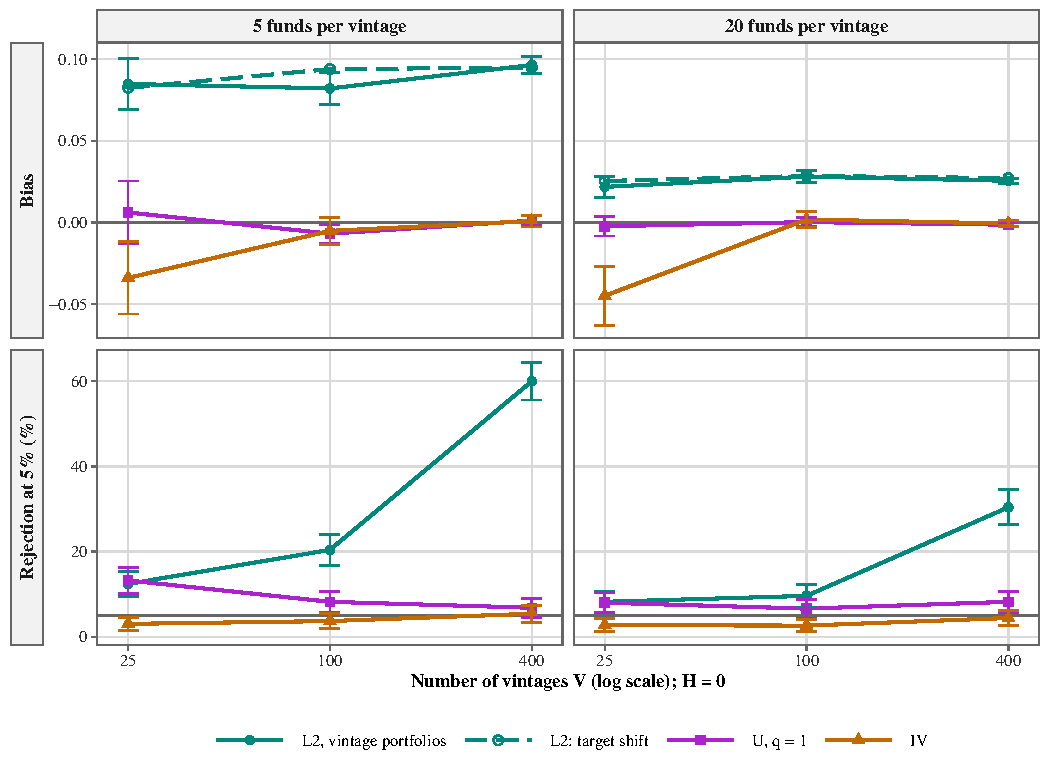
\includegraphics[width=0.85\textwidth]{figure_S3_growing_V.pdf}
\caption{Monte Carlo: more vintages with the same funds per vintage}
\label{fig:mc_growing_v}
\par\vspace{2pt}
{\scriptsize\textit{Notes:} Single-factor $\hat\beta_{MKT}$ (true value 1) at $H=0$ for $V=25$, 100 and 400 consecutive vintages ending 2005 with 5 or 20 funds each, deal model of the cores. Each replication draws its own factor path: whole months of 1967--2021 resampled i.i.d.\ on a calendar from the first vintage to 2021 (100 or 400 vintages do not fit the history). L2 on vintage portfolios with its target shift (the minimizer of the criterion averaged over replications 1--200, minus the true value); $U_{v,H}$ with $q_v=1$; IV as in Table~\ref{tab:mc_size_additions}. The L2 bias does not fall with $V$; it equals the target shift and shrinks with the funds per vintage (the noise tilt, T3/T4), and with a fixed bias and a shrinking SE its rejection rate rises with $V$. Bars: $\pm2$ Monte Carlo SE. 500 replications per design.}
\end{figure}


% ==============================================================================
\section{Comparison to \citet{DLP12}}
\label{sec:dlp_results_comparison}
% ==============================================================================

\subsection{Simulation comparison under pipeline r5}
\label{sec:dlp_simulation}

Table~\ref{tab:driessen_comparison} re-estimates all 19 scenarios of the \citet[Table~1]{DLP12} simulation comparison (Panels~A and~B, 1,000 replications per scenario) using the repaired estimator on the admissible domain $\Theta$ (pipeline r5). Within our simulator, Table~\ref{tab:mc_grid} isolates the $n_v \times V$ infill noise effect: at $H=0$, L2 bias falls sharply with funds per vintage $n_v$ and does not fall with the number of vintages $V$. Full cross-paper attribution of the remaining difference between Scenario~(S3) and \citet[Table~1]{DLP12} also reflects differences in the market-return process (simulated i.i.d.\ vs.\ historical path) and the return-linked shifted additive lognormal innovation.

% Auto-generated by r_project/simulation/mc_paper.R
% Generated 2026-11-27 03:56 at commit 8585b0d (uncommitted changes)
% Source: results/mc_step4/appendix_d_summary.csv (simulation/mc_appendix_d.R, commit(s) aa67c7a)

\begin{table}[htbp]
\centering
\caption{Comparison to simulation \cite[Table 1]{DLP12}}
\label{tab:driessen_comparison}
\resizebox{\linewidth}{!}{%
\begin{tabular}{l ccccc cccccc}
\toprule
& \multicolumn{5}{c}{Market Beta ($\beta$)} & \multicolumn{6}{c}{Alpha ($\alpha$, monthly \%)} \\
\cmidrule(lr){2-6} \cmidrule(lr){7-12}
Scenario & True & Mean & SD & 25\% & 75\% & True & Mean & SD & 25\% & 75\% & \% Bound \\
\midrule
\multicolumn{12}{l}{\textit{Panel A: mean-one multiplicative deal shocks}} \\
(S1) $n=20$, $\sigma=20\%$ & 1.00 & 0.94 & 0.40 & 0.74 & 1.18 & 0.00 & 0.14 & 0.27 & -0.01 & 0.22 & 0\% \\
(S2) $n=50$, $\sigma=20\%$ & 1.00 & 0.98 & 0.26 & 0.85 & 1.13 & 0.00 & 0.07 & 0.16 & -0.03 & 0.12 & 0\% \\
(S3) $n=50$, $\sigma=30\%$ & 1.00 & 0.76 & 0.70 & 0.32 & 1.21 & 0.00 & 0.48 & 0.65 & 0.00 & 0.78 & 8\% \\
(S5) $n=50$, $\sigma=30\%$, Sim.~MKT & 1.00 & 0.70 & 0.79 & 0.15 & 1.16 & 0.00 & 0.62 & 0.79 & 0.01 & 1.15 & 15\% \\
(S6) $n=50$, $\sigma=30\%$, Sim.~MKT, $\bar{\alpha}=1\%$ & 1.00 & 0.88 & 0.71 & 0.37 & 1.26 & 0.00 & 0.42 & 0.51 & 0.00 & 1.00 & 29\% \\
(S7) $n=50$, $\sigma=30\%$, Sim.~MKT, Det.~Timing & 1.00 & 0.74 & 0.80 & 0.23 & 1.20 & 0.00 & 0.60 & 0.81 & -0.02 & 1.18 & 16\% \\
(S8) $n=50$, $\sigma=30\%$, Sim.~MKT, Max.~Hold 5 & 1.00 & 0.89 & 0.57 & 0.58 & 1.18 & 0.00 & 0.29 & 0.54 & -0.04 & 0.48 & 3\% \\
(S9) $n=50$, $\sigma=30\%$, Sim.~MKT, Max.~Hold 5, Det.~Timing & 1.00 & 0.90 & 0.52 & 0.62 & 1.19 & 0.00 & 0.26 & 0.50 & -0.05 & 0.45 & 2\% \\
(S10) $n=50$, $\sigma=30\%$, Sim.~MKT, Max.~Hold 5, Det.~Timing, $\bar{\alpha}=1\%$ & 1.00 & 0.94 & 0.47 & 0.64 & 1.21 & 0.00 & 0.22 & 0.39 & -0.05 & 0.45 & 8\% \\
\addlinespace
\multicolumn{12}{l}{\textit{Panel B: additive deal shocks with default truncation (former shock model)}} \\
(S1) $n=20$, $\sigma=20\%$, Normal & 1.00 & 0.93 & 0.40 & 0.72 & 1.17 & 0.00 & 0.15 & 0.28 & -0.01 & 0.24 & 1\% \\
(S2) $n=50$, $\sigma=20\%$, Normal & 1.00 & 0.98 & 0.26 & 0.85 & 1.12 & 0.00 & 0.07 & 0.16 & -0.02 & 0.13 & 0\% \\
(S3) $n=50$, $\sigma=30\%$, Normal & 1.00 & 0.68 & 0.71 & 0.21 & 1.16 & 0.00 & 0.58 & 0.71 & 0.03 & 0.97 & 12\% \\
(S4) $n=50$, $\sigma=30\%$, Shifted LN & 1.00 & 0.75 & 0.69 & 0.31 & 1.19 & 0.00 & 0.47 & 0.65 & 0.00 & 0.75 & 8\% \\
(S5) $n=50$, $\sigma=30\%$, Shifted LN, Sim.~MKT & 1.00 & 0.70 & 0.78 & 0.17 & 1.17 & 0.00 & 0.61 & 0.78 & 0.01 & 1.08 & 15\% \\
(S6) $n=50$, $\sigma=30\%$, Shifted LN, Sim.~MKT, $\bar{\alpha}=1\%$ & 1.00 & 0.87 & 0.69 & 0.36 & 1.24 & 0.00 & 0.41 & 0.51 & 0.01 & 1.00 & 28\% \\
(S7) $n=50$, $\sigma=30\%$, Shifted LN, Sim.~MKT, Det.~Timing & 1.00 & 0.74 & 0.80 & 0.24 & 1.19 & 0.00 & 0.58 & 0.80 & -0.04 & 1.14 & 15\% \\
(S8) $n=50$, $\sigma=30\%$, Shifted LN, Sim.~MKT, Max.~Hold 5 & 1.00 & 0.89 & 0.56 & 0.58 & 1.17 & 0.00 & 0.28 & 0.52 & -0.04 & 0.46 & 2\% \\
(S9) $n=50$, $\sigma=30\%$, Shifted LN, Sim.~MKT, Max.~Hold 5, Det.~Timing & 1.00 & 0.90 & 0.50 & 0.63 & 1.19 & 0.00 & 0.25 & 0.48 & -0.05 & 0.42 & 2\% \\
(S10) $n=50$, $\sigma=30\%$, Shifted LN, Sim.~MKT, Max.~Hold 5, Det.~Timing, $\bar{\alpha}=1\%$ & 1.00 & 0.94 & 0.46 & 0.66 & 1.19 & 0.00 & 0.21 & 0.38 & -0.05 & 0.42 & 7\% \\
\addlinespace
\multicolumn{12}{l}{\textit{Driessen et al. 2012, Table 1}} \\
Benchmark Estimates ($n=50$, $\sigma_{\text{monthly}}=30\%$) & 1.00 & 0.98 & 0.32 & 0.80 & 1.15 & 0.00 & 0.05 & 0.2 & -0.06 & 0.15 & n/a \\
\bottomrule
\end{tabular}%
}
\par\vspace{2pt}
{\scriptsize\textit{Notes:} Small-sample properties at $H=0$ of the estimator of the paper's tables: L2 on equally weighted vintage-year portfolios, $(\alpha,\beta)$ minimized over the admissible domain ($\beta\in[-1,4]$, $\alpha\le\bar\alpha$, gross benchmark return at least 0.08 in every month of the window; constrained multi-start minimizer), mimicking Table~1 of \cite{DLP12}. 1{,}000 Monte Carlo samples per scenario. All scenarios: 20 vintage years (1986--2005), 15 deals per fund, investment period 5 years; unless stated otherwise $n=20$ funds per vintage, $\sigma=20\%$ monthly deal volatility, a normal shock, the historical factor path, random deal timing, holding periods up to 10 years and $\bar\alpha=2\%$ per month. Panel~A: deal payoffs compound over the months after the investment month with mean-one lognormal monthly shocks, $G_u(1+\varepsilon_u)$, $\mathrm{E}[1+\varepsilon_u]=1$, so the process prices exactly at the true parameters; normal and shifted-lognormal shocks then coincide and (S4) equals (S3). Panel~B: the former additive shocks $G_u+\varepsilon_u$ with default truncation (a deal path below zero pays nothing), which raises the expected payoff above the benchmark. $n$: funds per vintage; $\sigma$: monthly deal volatility; \textit{Shifted LN}: shifted lognormal shock (cf.\ \cite{DLP12}); \textit{Sim.~MKT}: total market return i.i.d.\ shifted lognormal (S\&P~500 1980--2003 moments), risk-free rate 4\% per year; \textit{Det.~Timing}: evenly spaced deal investment dates; \textit{Max.~Hold 5}: holding periods up to 5 years; $\bar\alpha$: upper bound on $\alpha$. \textit{\% Bound}: share of samples whose estimate lies on the boundary of the domain (an active constraint): almost always $\alpha=\bar\alpha$; $\beta$ at $-1$ or 4 in at most 1.7\% of samples, the gross floor never. Alpha in monthly percent. The last row: the benchmark estimates of \cite[Table~1]{DLP12}. Within our simulator, Table~\ref{tab:mc_grid} isolates the $n_v\times V$ infill noise effect; full cross-paper attribution of the gap between (S3) and \cite[Table~1]{DLP12} also reflects DLP12's simulated market and return-linked shifted additive lognormal innovation.}
\end{table}


% ==============================================================================
\section{Additional Empirical Exhibits and Step 5 Diagnostics}
\label{sec:appendix_empirical_extra}
% ==============================================================================

This appendix collects the complete 12-horizon single-factor table (Table~\ref{tab:u_l2_beta_all}), the VC cohort diagnostic excluding 1993--1997 (Table~\ref{tab:vc_without_1993_1997}), the three-rule fund-size imputation sensitivity (Table~\ref{tab:fw_imputation_sensitivity}), sample robustness across complete histories, all funds, and the 20\% terminal-NAV early-stopper filter for both L2 and $U_{v,H}$ (Table~\ref{tab:robustness_samples}), the Fix-$A$ vs.\ Scale-Jacobian decomposition (Table~\ref{tab:fixA_jacobian}), joint $(\alpha,\beta)$ geometry and contours (Table~\ref{tab:alpha_beta_identification} and Figure~\ref{fig:alpha_beta_contours}), four-year overlapping vintage-block bootstrap intervals (Table~\ref{tab:block_bootstrap}), vintage-level residuals and booked terminal NAV shares (Figure~\ref{fig:vintage_residuals} and Table~\ref{tab:terminal_nav_shares}), $hv$-block cross-validation fold diagnostics (Table~\ref{tab:appendix_e_cv_folds}), two-factor $q^5$ empirical horizon profiles (Figures~\ref{fig:empirical_BO_q_factors} and~\ref{fig:empirical_VC_q_factors}), and a comparison with published Buyout and VC risk/return estimates (Table~\ref{tab:published_estimates}).

% Auto-generated by r_project/results/main_exhibits_u.R at commit 20f28de (uncommitted changes)
% Estimation results: L2 commit(s) ab0495c; U_{v,H} commit(s) ab0495c; no estimation in this script

\begin{table}[htbp]
\centering
\footnotesize
\caption{Single-factor $\hat\beta_{MKT}$: $U_{v,H}$ and L2, all horizons}
\label{tab:u_l2_beta_all}
\begin{tabular}{l rr rr rr rr}
\toprule
 & \multicolumn{4}{c}{Equally weighted funds (EW)} & \multicolumn{4}{c}{Fund-size weighted funds (FW)} \\
\cmidrule(lr){2-5} \cmidrule(lr){6-9}
 & \multicolumn{2}{c}{$U_{v,H}$ (main)} & \multicolumn{2}{c}{L2} & \multicolumn{2}{c}{$U_{v,H}$ (main)} & \multicolumn{2}{c}{L2} \\
\cmidrule(lr){2-3} \cmidrule(lr){4-5} \cmidrule(lr){6-7} \cmidrule(lr){8-9}
Horizon & $\hat\beta$ & SE & $\hat\beta$ & SE & $\hat\beta$ & SE & $\hat\beta$ & SE \\
\midrule
\multicolumn{9}{l}{\textit{Buyout}} \\
\quad 0 yr & 1.147$^{***}$ & 0.118 & 1.283 & 0.088 & 1.205$^{***}$ & 0.138 & 1.192 & 0.150 \\
\quad 2.5 yr & 1.146$^{***}$ & 0.121 & 1.272 & 0.090 & 1.213$^{***}$ & 0.155 & 1.179 & 0.184 \\
\quad 5 yr & 1.154$^{***}$ & 0.110 & 1.259 & 0.085 & 1.206$^{***}$ & 0.132 & 1.140 & 0.175 \\
\quad 10 yr & 1.158$^{***}$ & 0.072 & 1.157 & 0.079 & 1.227$^{***}$ & 0.069 & 0.988 & 0.152 \\
\quad 12.5 yr & 1.184$^{***}$ & 0.075 & 1.134 & 0.069 & 1.278$^{***}$ & 0.069 & 0.912 & 0.157 \\
\quad 15 yr & 1.268$^{***}$ & 0.137 & 1.108 & 0.060 & 1.404$^{***}$ & 0.164 & 0.827 & 0.151 \\
\quad 17.5 yr & 1.265$^{***}$ & 0.155 & 1.070 & 0.062 & 1.392$^{***}$ & 0.175 & 0.763 & 0.136 \\
\quad 20 yr & 1.239$^{***}$ & 0.172 & 1.018 & 0.085 & 1.368$^{***}$ & 0.197 & 0.698 & 0.127 \\
\quad 22.5 yr & 1.271$^{***}$ & 0.202 & 1.001 & 0.094 & 1.403$^{***}$ & 0.224 & 0.658 & 0.124 \\
\quad 25 yr & 1.254$^{***}$ & 0.173 & 0.988 & 0.091 & 1.372$^{***}$ & 0.190 & 0.631 & 0.119 \\
\quad 27.5 yr & 1.265$^{***}$ & 0.152 & 0.969 & 0.084 & 1.395$^{***}$ & 0.168 & 0.600 & 0.112 \\
\quad 30 yr & 1.309$^{***}$ & 0.159 & 0.933 & 0.080 & 1.458$^{***}$ & 0.178 & 0.558 & 0.103 \\
\addlinespace
\multicolumn{9}{l}{\textit{Venture capital}} \\
\quad 0 yr & 1.493$^{**}$ & 0.325 & 1.925 & 0.379 & 1.649$^{**}$ & 0.338 & 2.089 & 0.376 \\
\quad 2.5 yr & 1.653$^{**}$ & 0.367 & 2.143 & 0.357 & 1.832$^{**}$ & 0.347 & 2.314 & 0.318 \\
\quad 5 yr & 1.992$^{*}$ & 0.525 & 2.145 & 0.390 & 2.191$^{**}$ & 0.467 & 2.320 & 0.333 \\
\quad 10 yr & 1.655$^{*}$ & 0.465 & 1.710 & 0.389 & 1.810$^{*}$ & 0.456 & 1.864 & 0.385 \\
\quad 12.5 yr & 1.382$^{*}$ & 0.371 & 1.482 & 0.401 & 1.512$^{*}$ & 0.389 & 1.636 & 0.424 \\
\quad 15 yr & 1.250$^{*}$ & 0.350 & 1.270 & 0.410 & 1.367$^{*}$ & 0.372 & 1.401 & 0.444 \\
\quad 17.5 yr & 1.222$^{*}$ & 0.349 & 1.083 & 0.428 & 1.339$^{*}$ & 0.374 & 1.199 & 0.465 \\
\quad 20 yr & 1.192$^{*}$ & 0.377 & 0.943 & 0.473 & 1.302$^{*}$ & 0.412 & 1.044 & 0.529 \\
\quad 22.5 yr & 1.177 & 0.453 & 0.701 & 0.517 & 1.276 & 0.503 & 0.717 & 0.607 \\
\quad 25 yr & 1.194 & 0.650 & 0.026 & 0.304 & 1.248 & 0.779 & -0.157 & 0.318 \\
\quad 27.5 yr & 1.339 & 1.339 & -0.316 & 0.284 & 1.444 & 2.035 & -0.417 & 0.281 \\
\quad 30 yr & 0.760 & 2.116 & -0.373 & 0.272 & 0.121 & 0.655 & -0.450 & 0.273 \\
\bottomrule
\end{tabular}
\par\vspace{2pt}
{\scriptsize\textit{Notes:} Single-factor $\hat\beta_{MKT}$. North America, vintages up to 2010: Buyout 25 vintages; VC 27, of which the 23 with at least two funds enter $U_{v,H}$. $U_{v,H}$: the cross-fund pair-product criterion with equal vintage weights ($q_v=1$); without shared vintage effects and with the expected pricing error zero given the benchmark path, it targets the true parameter at every horizon, $H=0$ included. L2: squared loss on vintage portfolios (DLP12 at $H=0$), whose target is tilted by within-vintage fund noise and moves with $H$. SE: Bartlett sandwich over vintage years, $S=\lceil1.3\sqrt V\rceil$. Markers on $U_{v,H}$: two-sided fixed-$b$ $p$-values of a test of zero, $^{*}$\,$p<0.05$, $^{**}$\,$p<0.01$, $^{***}$\,$p<0.001$. $^{\dagger}$: estimate on a bound of the admissible domain ($\beta\in[-1,4]$, $\alpha\in[-2\%,2\%]$ per month, gross benchmark return at least 0.08), no SE. The headline estimate is $U_{v,H}$ at $H=0$; the horizon changes the weights of the vintages, not the target of $U_{v,H}$, and in a Monte Carlo shaped like our data its precision falls with $H$.}
\end{table}

% Auto-generated by r_project/results/main_exhibits_u.R at commit 4bd0e9c (uncommitted changes)
% Estimation results: L2 commit(s) 731ea2f (run with uncommitted changes); U_{v,H} commit(s) 731ea2f; no estimation in this script

\begin{table}[htbp]
\centering
\footnotesize
\caption{Venture capital, $(\alpha,\beta)$ model: full sample and without the 1993--1997 vintages}
\label{tab:vc_without_1993_1997}
\begin{tabular}{l rr rr}
\toprule
 & \multicolumn{2}{c}{Full sample (27 vintages)} & \multicolumn{2}{c}{Without 1993--1997 (22 vintages)} \\
\cmidrule(lr){2-3} \cmidrule(lr){4-5}
Horizon & $\hat\beta$ & $\hat\alpha$ & $\hat\beta$ & $\hat\alpha$ \\
\midrule
\multicolumn{5}{l}{\textit{$U_{v,H}$ ($q_v=1$), equally weighted}} \\
\quad 0 yr & -0.080$^{\dagger}$ & 2.000$^{\dagger}$ & 1.666 & -0.522 \\
\quad 2.5 yr & 1.180 & 0.501 & 1.706 & -0.522 \\
\quad 5 yr & 1.702 & 0.391 & 1.786 & -0.549 \\
\quad 10 yr & 1.599 & 0.053 & 1.842 & -0.598 \\
\quad 15 yr & 1.810 & -0.469 & 1.853 & -0.723 \\
\quad 20 yr & 2.005 & -0.659 & 1.832 & -0.714 \\
\quad 30 yr & 2.169 & -0.997 & 1.958 & -0.809 \\
\addlinespace
\multicolumn{5}{l}{\textit{L2, equally weighted}} \\
\quad 0 yr & 0.674$^{\dagger}$ & 2.000$^{\dagger}$ & 1.693 & -0.422 \\
\quad 2.5 yr & 1.568 & 0.813 & 1.750 & -0.439 \\
\quad 5 yr & 1.631 & 0.672 & 1.804 & -0.509 \\
\quad 10 yr & 1.961 & -0.238 & 1.969 & -0.679 \\
\quad 15 yr & 2.232 & -0.787 & 1.973 & -0.850 \\
\quad 20 yr & 2.345 & -1.052 & 2.027 & -1.024 \\
\quad 30 yr & 2.342 & -1.334 & 2.168 & -1.151 \\
\addlinespace
\multicolumn{5}{l}{\textit{$U_{v,H}$ ($q_v=1$), fund-size weighted}} \\
\quad 0 yr & 0.368$^{\dagger}$ & 2.000$^{\dagger}$ & 1.607 & -0.495 \\
\quad 2.5 yr & 1.257 & 0.919 & 1.609 & -0.489 \\
\quad 5 yr & 2.081 & 0.640 & 1.690 & -0.524 \\
\quad 10 yr & 1.863 & 0.039 & 1.815 & -0.585 \\
\quad 15 yr & 2.065 & -0.557 & 1.817 & -0.684 \\
\quad 20 yr & 2.238 & -0.747 & 1.785 & -0.667 \\
\quad 30 yr & 2.327 & -1.133 & 1.881 & -0.719 \\
\addlinespace
\multicolumn{5}{l}{\textit{L2, fund-size weighted}} \\
\quad 0 yr & 1.169$^{\dagger}$ & 2.000$^{\dagger}$ & 1.649 & -0.422 \\
\quad 2.5 yr & 1.610 & 1.670 & 1.672 & -0.435 \\
\quad 5 yr & 1.892 & 1.189 & 1.734 & -0.507 \\
\quad 10 yr & 2.234 & -0.192 & 1.937 & -0.668 \\
\quad 15 yr & 2.534 & -0.854 & 1.945 & -0.821 \\
\quad 20 yr & 2.633 & -1.120 & 2.018 & -1.005 \\
\quad 30 yr & 2.536 & -1.470 & 2.180 & -1.124 \\
\bottomrule
\end{tabular}
\par\vspace{2pt}
{\scriptsize\textit{Notes:} Point estimates only, as a description: the block of vintages was chosen after looking at the data (it is the group of vintages whose terms push the criterion down in $\alpha$ at the $H=0$ estimate), so no inference is reported. $\hat\alpha$ in percent per month. Full sample: the estimates of Table~\ref{tab:u_l2_alpha_beta}. Vintage counts in the header are those of L2; $U_{v,H}$ uses the vintages with at least two funds. Same estimators, domain and data as there; refits on the vintages outside 1993--1997. $^{\dagger}$: estimate on a bound of the admissible domain.}
\end{table}

% Auto-generated by r_project/results/fw_imputation_sensitivity.R at commit 8585b0d (uncommitted changes)
\begin{table}[htbp]
\centering
\footnotesize
\caption{Fund-size imputation sensitivity for fund-size weighted (FW) single-factor $\hat\beta_{MKT}$}
\label{tab:fw_imputation_sensitivity}
\resizebox{\linewidth}{!}{%
\begin{tabular}{l r c rrr rrr rr}
\toprule
 & & & \multicolumn{3}{c}{$U_{v,H}$, $q_v=1$} & \multicolumn{3}{c}{L2, vintage portfolios} & L2 decline & $H=0$ gap \\
\cmidrule(lr){4-6} \cmidrule(lr){7-9}
Imputation rule & Funds & $V_{\mathrm{L2}}/V_U$ & $H=0$ & 15 yr & 30 yr & $H=0$ & 15 yr & 30 yr & 0--30 yr & L2$-U_{v,H}$ \\
\midrule
\multicolumn{11}{l}{\textit{Buyout, fund-size weighted (FW)}} \\
\quad Within-vintage median (baseline) & 383 & 25/25 & 1.197 & 1.379 & 1.428 & 1.224 & 0.989 & 0.798 & 0.427 & 0.028 \\
\quad Pooled cross-vintage mean & 383 & 25/25 & 1.205 & 1.404 & 1.458 & 1.192 & 0.827 & 0.558 & 0.634 & -0.013 \\
\quad Drop missing-size funds & 373 & 25/22 & 1.226 & 1.292 & 1.393 & 1.381 & 1.201 & 0.962 & 0.419 & 0.155 [0.042] \\
\addlinespace
\multicolumn{11}{l}{\textit{Venture capital, fund-size weighted (FW)}} \\
\quad Within-vintage median (baseline) & 432 & 27/23 & 1.742 & 1.423 & -0.076 & 2.287 & 1.595 & -0.573 & 2.860 & 0.546 [0.551] \\
\quad Pooled cross-vintage mean & 432 & 27/23 & 1.649 & 1.367 & 0.121 & 2.089 & 1.401 & -0.450 & 2.539 & 0.440 [0.445] \\
\quad Drop missing-size funds & 417 & 26/22 & 1.807 & 1.543 & -0.173 & 2.364 & 1.791 & -0.605 & 2.969 & 0.557 [0.566] \\
\bottomrule
\end{tabular}%
}
\par\vspace{2pt}
{\scriptsize\textit{Notes:} North America, complete-history sample, vintages up to 2010 (10 of 383 Buyout funds and 15 of 432 VC funds lack reported fund size in Preqin, concentrated in early small vintages). \textit{Within-vintage median (baseline)}: imputes missing sizes using the observed median fund size in the same vintage (expanding symmetrically to nearest vintages when a vintage has no observed size, e.g.\ singleton 1982 VC). \textit{Pooled cross-vintage mean}: imputes the pooled strategy mean (\$1{,}842M Buyout, \$379M VC), which assigns up to 94.9\% weight to a single missing-size Buyout fund in 1986 and 98.8\% to two missing-size VC funds in 1985. \textit{Drop missing-size funds}: excludes missing-size funds, shrinking Buyout $U_{v,H}$ from 25 to 22 vintages while L2 stays at 25 (and VC from 27/23 to 26/22). Where $V_{\mathrm{L2}}\neq V_U$, the $H=0$ L2$-U_{v,H}$ gap is shown for full-sample L2 followed in brackets by matched-vintage ($V_U$) L2. Joint $(\alpha,\beta)$ sensitivity rows are saved in \texttt{fw\_imputation\_sensitivity.csv}.}
\end{table}

% Auto-generated by r_project/results/robustness_samples.R at commit 8585b0d (uncommitted changes)
\begin{table}[htbp]
\centering
\footnotesize
\renewcommand{\arraystretch}{0.92}
\caption{Sample robustness: complete histories, all funds, and without early stoppers with large terminal NAV}
\label{tab:robustness_samples}
\resizebox{\linewidth}{!}{%
\begin{tabular}{l r rrr rrr}
\toprule
\multicolumn{8}{l}{\textit{Panel A: single-factor $\hat\beta_{MKT}$ (SE)}} \\
 & & \multicolumn{3}{c}{L2, vintage portfolios} & \multicolumn{3}{c}{$U_{v,H}$, $q_v=1$} \\
\cmidrule(lr){3-5} \cmidrule(lr){6-8}
Sample & Funds & $H=0$ & 15 yr & 30 yr & $H=0$ & 15 yr & 30 yr \\
\midrule
\multicolumn{8}{l}{\textit{Buyout, equally weighted}} \\
\quad Complete histories (main) & 383 & 1.283 (0.088) & 1.108 (0.060) & 0.933 (0.080) & 1.147 (0.118) & 1.268 (0.137) & 1.309 (0.159) \\
\quad All funds & 495 & 1.257 (0.084) & 1.066 (0.058) & 0.908 (0.062) & 1.105 (0.128) & 1.247 (0.130) & 1.304 (0.145) \\
\quad Without early stoppers, NAV $>20\%$ & 328 & 1.301 (0.080) & 1.134 (0.072) & 0.933 (0.082) & 1.179 (0.118) & 1.290 (0.137) & 1.305 (0.159) \\
\multicolumn{8}{l}{\textit{Buyout, fund-size weighted}} \\
\quad Complete histories (main) & 383 & 1.224 (0.126) & 0.989 (0.100) & 0.798 (0.079) & 1.197 (0.143) & 1.379 (0.157) & 1.428 (0.173) \\
\quad All funds & 495 & 1.217 (0.131) & 1.006 (0.106) & 0.841 (0.100) & 1.208 (0.141) & 1.376 (0.117) & 1.503 (0.127) \\
\quad Without early stoppers, NAV $>20\%$ & 328 & 1.280 (0.141) & 1.005 (0.110) & 0.775 (0.093) & 1.259 (0.161) & 1.392 (0.151) & 1.411 (0.177) \\
\multicolumn{8}{l}{\textit{Venture capital, equally weighted}} \\
\quad Complete histories (main) & 432 & 1.925 (0.379) & 1.270 (0.410) & -0.373 (0.272) & 1.493 (0.325) & 1.250 (0.350) & 0.760 (2.116) \\
\quad All funds & 538 & 1.881 (0.331) & 1.195 (0.416) & -0.431 (0.249) & 1.506 (0.308) & 1.203 (0.361) & 0.175 (0.578) \\
\quad Without early stoppers, NAV $>20\%$ & 344 & 2.111 (0.389) & 1.429 (0.458) & -0.421 (0.280) & 1.657 (0.354) & 1.360 (0.354) & 0.203 (0.696) \\
\multicolumn{8}{l}{\textit{Venture capital, fund-size weighted}} \\
\quad Complete histories (main) & 432 & 2.287 (0.384) & 1.595 (0.485) & -0.573 (0.252) & 1.742 (0.342) & 1.423 (0.387) & -0.076 (0.431) \\
\quad All funds & 538 & 2.263 (0.354) & 1.544 (0.497) & -0.614 (0.235) & 1.725 (0.324) & 1.377 (0.399) & -0.130 (0.411) \\
\quad Without early stoppers, NAV $>20\%$ & 344 & 2.406 (0.379) & 1.727 (0.524) & -0.589 (0.255) & 1.877 (0.359) & 1.509 (0.390) & -0.142 (0.395) \\
\midrule
\multicolumn{8}{l}{\textit{Panel B: $(\alpha,\beta)$ model, L2 on vintage portfolios: $\hat\beta_{MKT}$ (SE) and $\hat\alpha$ in monthly \% (SE)}} \\
 & \multicolumn{2}{c}{$H=0$} & \multicolumn{2}{c}{15 yr} & \multicolumn{2}{c}{30 yr} & \\
\cmidrule(lr){2-3} \cmidrule(lr){4-5} \cmidrule(lr){6-7}
Sample & $\hat\beta$ & $\hat\alpha$ & $\hat\beta$ & $\hat\alpha$ & $\hat\beta$ & $\hat\alpha$ & \\
\midrule
\multicolumn{8}{l}{\textit{Buyout, equally weighted}} \\
\quad Complete histories (main) & 0.494 (0.143) & 0.635 (0.125) & 0.510 (0.158) & 0.455 (0.112) & 1.065 (0.506) & -0.111 (0.388) & \\
\quad All funds & 0.507 (0.160) & 0.601 (0.135) & 0.546 (0.167) & 0.401 (0.115) & 1.160 (0.491) & -0.210 (0.382) & \\
\quad Without early stoppers, NAV $>20\%$ & 0.475 (0.170) & 0.670 (0.138) & 0.537 (0.166) & 0.448 (0.108) & 1.054 (0.517) & -0.100 (0.394) & \\
\multicolumn{8}{l}{\textit{Buyout, fund-size weighted}} \\
\quad Complete histories (main) & 0.420 (0.157) & 0.668 (0.165) & 0.579 (0.225) & 0.320 (0.196) & 0.900 (0.387) & -0.082 (0.282) & \\
\quad All funds & 0.402 (0.184) & 0.690 (0.168) & 0.567 (0.244) & 0.353 (0.189) & 0.950 (0.403) & -0.089 (0.297) & \\
\quad Without early stoppers, NAV $>20\%$ & 0.341 (0.199) & 0.792 (0.211) & 0.558 (0.247) & 0.352 (0.221) & 0.874 (0.414) & -0.084 (0.296) & \\
\multicolumn{8}{l}{\textit{Venture capital, equally weighted}} \\
\quad Complete histories (main) & 0.674$^\dagger$ (--) & 2.000$^\dagger$ (--) & 2.232 (0.236) & -0.787 (0.111) & 2.342 (0.196) & -1.334 (0.106) & \\
\quad All funds & 0.643$^\dagger$ (--) & 2.000$^\dagger$ (--) & 2.265 (0.220) & -0.822 (0.115) & 2.362 (0.220) & -1.361 (0.086) & \\
\quad Without early stoppers, NAV $>20\%$ & 0.904$^\dagger$ (--) & 2.000$^\dagger$ (--) & 2.307 (0.251) & -0.774 (0.120) & 2.330 (0.191) & -1.369 (0.126) & \\
\multicolumn{8}{l}{\textit{Venture capital, fund-size weighted}} \\
\quad Complete histories (main) & 1.169$^\dagger$ (--) & 2.000$^\dagger$ (--) & 2.534 (0.235) & -0.854 (0.109) & 2.536 (0.164) & -1.470 (0.107) & \\
\quad All funds & 1.171$^\dagger$ (--) & 2.000$^\dagger$ (--) & 2.556 (0.223) & -0.865 (0.111) & 2.554 (0.166) & -1.485 (0.095) & \\
\quad Without early stoppers, NAV $>20\%$ & 1.301$^\dagger$ (--) & 2.000$^\dagger$ (--) & 2.582 (0.243) & -0.838 (0.125) & 2.527 (0.173) & -1.496 (0.118) & \\
\midrule
\multicolumn{8}{l}{\textit{Panel C: $(\alpha,\beta)$ model, $U_{v,H}$ ($q_v=1$): $\hat\beta_{MKT}$ (SE) and $\hat\alpha$ in monthly \% (SE)}} \\
 & \multicolumn{2}{c}{$H=0$} & \multicolumn{2}{c}{15 yr} & \multicolumn{2}{c}{30 yr} & \\
\cmidrule(lr){2-3} \cmidrule(lr){4-5} \cmidrule(lr){6-7}
Sample & $\hat\beta$ & $\hat\alpha$ & $\hat\beta$ & $\hat\alpha$ & $\hat\beta$ & $\hat\alpha$ & \\
\midrule
\multicolumn{8}{l}{\textit{Buyout, equally weighted}} \\
\quad Complete histories (main) & 0.362 (0.207) & 0.605 (0.145) & 0.536 (0.347) & 0.523 (0.227) & -1.000$^\dagger$ (--) & 1.914$^\dagger$ (--) & \\
\quad All funds & 0.400 (0.198) & 0.551 (0.147) & 0.631 (0.319) & 0.444 (0.207) & -1.000$^\dagger$ (--) & 1.948$^\dagger$ (--) & \\
\quad Without early stoppers, NAV $>20\%$ & 0.357 (0.241) & 0.637 (0.164) & 0.551 (0.380) & 0.521 (0.246) & -1.000$^\dagger$ (--) & 1.911$^\dagger$ (--) & \\
\multicolumn{8}{l}{\textit{Buyout, fund-size weighted}} \\
\quad Complete histories (main) & 0.439 (0.178) & 0.568 (0.192) & 0.971 (0.592) & 0.267 (0.364) & -0.873 (1.152) & 1.785 (1.029) & \\
\quad All funds & 0.485 (0.203) & 0.558 (0.194) & 0.935 (0.396) & 0.303 (0.272) & -1.000$^\dagger$ (--) & 1.962$^\dagger$ (--) & \\
\quad Without early stoppers, NAV $>20\%$ & 0.364 (0.227) & 0.681 (0.242) & 0.914 (0.625) & 0.314 (0.405) & -0.820 (1.057) & 1.738 (0.928) & \\
\multicolumn{8}{l}{\textit{Venture capital, equally weighted}} \\
\quad Complete histories (main) & -0.080$^\dagger$ (--) & 2.000$^\dagger$ (--) & 1.810 (0.213) & -0.469 (0.241) & 2.169 (0.225) & -0.997 (0.139) & \\
\quad All funds & -0.034$^\dagger$ (--) & 2.000$^\dagger$ (--) & 1.901 (0.210) & -0.553 (0.208) & 2.208 (0.228) & -1.049 (0.124) & \\
\quad Without early stoppers, NAV $>20\%$ & 0.150$^\dagger$ (--) & 2.000$^\dagger$ (--) & 1.905 (0.223) & -0.464 (0.232) & 2.215 (0.194) & -1.033 (0.165) & \\
\multicolumn{8}{l}{\textit{Venture capital, fund-size weighted}} \\
\quad Complete histories (main) & 0.368$^\dagger$ (--) & 2.000$^\dagger$ (--) & 2.065 (0.195) & -0.557 (0.191) & 2.327 (0.180) & -1.133 (0.134) & \\
\quad All funds & 0.345$^\dagger$ (--) & 2.000$^\dagger$ (--) & 2.098 (0.185) & -0.587 (0.189) & 2.353 (0.185) & -1.141 (0.125) & \\
\quad Without early stoppers, NAV $>20\%$ & 0.542$^\dagger$ (--) & 2.000$^\dagger$ (--) & 2.150 (0.217) & -0.558 (0.185) & 2.352 (0.172) & -1.159 (0.150) & \\
\bottomrule
\end{tabular}%
}
\par\vspace{2pt}
{\scriptsize\textit{Notes:} North America, vintages up to 2010, the estimators of the main tables (r5 domain, Bartlett sandwich SE with $S=\lceil1.3\sqrt V\rceil$, no cross-validation). \textit{Complete histories}: the main sample (a fund's last record lies more than 5 years after its vintage year starts, or it still reports at the data end). \textit{All funds}: adds the truncated histories. \textit{Without early stoppers}: the main sample without funds that stop reporting after age 5 and before 2021-03-31 with a last reported NAV above 20\% of total value (distributions plus that NAV). In Panel~C, VC $U_{v,H}$ sits on the $+2\%$ monthly $\alpha$ cap at $H=0$ across all three samples while FW $\hat\beta$ shifts noticeably under the NAV-threshold trim. Funds: funds in the sample's vintage portfolios. $^\dagger$: estimate on the boundary of the admissible domain, no SE.}
\end{table}

% Auto-generated by r_project/results/step5_diagnostics.R at commit 8585b0d (uncommitted changes)

\begin{table}[htbp]
\centering
\footnotesize
\caption{Horizon profile of L2: Fix-$A$ re-weighting versus the Scale-Jacobian penalty (Theorem~1, T5)}
\label{tab:fixA_jacobian}
\begin{tabular}{l rrr rrr}
\toprule
 & \multicolumn{3}{c}{Point estimates} & \multicolumn{3}{c}{L2 slope $\partial_\beta Q_H$ at $\hat\beta_{U,0}$} \\
\cmidrule(lr){2-4} \cmidrule(lr){5-7}
Horizon & L2 $\hat\beta_H$ & Fix-$A$ $\hat\beta_H^{\mathrm{Fix}A}$ & $\hat\beta_H-\hat\beta_H^{\mathrm{Fix}A}$ & Term~(I) Disc. & Term~(II) Jac. & Total \\
\midrule
\multicolumn{7}{l}{\textit{Buyout, equally weighted (evaluated at $\hat\beta_{U,0}=1.147$)}} \\
\quad 0 yr & 1.283 & 1.283 & 0.000 & -0.02 & 0.00 & -0.02 \\
\quad 5 yr & 1.259 & 1.329 & -0.071 & -0.05 & 0.02 & -0.03 \\
\quad 15 yr & 1.108 & 1.292 & -0.184 & -0.17 & 0.21 & 0.05 \\
\quad 30 yr & 0.933 & 1.266 & -0.334 & -0.44 & 1.24 & 0.79 \\
\addlinespace
\multicolumn{7}{l}{\textit{Buyout, fund-size weighted (evaluated at $\hat\beta_{U,0}=1.197$)}} \\
\quad 0 yr & 1.224 & 1.224 & 0.000 & 0.00 & 0.00 & 0.00 \\
\quad 5 yr & 1.218 & 1.286 & -0.069 & -0.02 & 0.02 & -0.01 \\
\quad 15 yr & 0.989 & 1.156 & -0.167 & 0.05 & 0.23 & 0.28 \\
\quad 30 yr & 0.798 & 1.106 & -0.308 & 0.37 & 1.43 & 1.80 \\
\addlinespace
\multicolumn{7}{l}{\textit{Venture capital, equally weighted (evaluated at $\hat\beta_{U,0}=1.493$)}} \\
\quad 0 yr & 1.925 & 1.925 & 0.000 & -0.13 & 0.00 & -0.13 \\
\quad 5 yr & 2.145 & 2.466 & -0.321 & -0.79 & 0.53 & -0.27 \\
\quad 15 yr & 1.270 & 2.030 & -0.760 & -1.55 & 2.22 & 0.67 \\
\quad 30 yr & -0.373 & 2.256 & -2.629 & -10.67 & 22.93 & 12.25 \\
\addlinespace
\multicolumn{7}{l}{\textit{Venture capital, fund-size weighted (evaluated at $\hat\beta_{U,0}=1.742$)}} \\
\quad 0 yr & 2.287 & 2.287 & 0.000 & -0.21 & 0.00 & -0.21 \\
\quad 5 yr & 2.472 & 2.914 & -0.441 & -1.76 & 1.28 & -0.49 \\
\quad 15 yr & 1.595 & 2.423 & -0.829 & -3.33 & 3.94 & 0.60 \\
\quad 30 yr & -0.573 & 2.680 & -3.253 & -27.15 & 47.72 & 20.57 \\
\bottomrule
\end{tabular}
\par\vspace{2pt}
{\scriptsize\textit{Notes:} North America complete-history sample ($V\le 2010$). Fix-$A$ minimizes $V^{-1}\sum_v A_{v,H}(\hat\beta_{U,0})^2 PV_v(\beta)^2$, isolating pure vintage re-weighting without the $\beta$-dependence of $A_{v,H}(\beta)$. The difference $\hat\beta_H - \hat\beta_H^{\mathrm{Fix}A}$ measures the pull of the Scale-Jacobian term (Theorem~1, T5). Right panel: exact decomposition of $\partial_\beta Q_H(\beta)$ at $\hat\beta_{U,0}$ into Term~(I) Inception Discounting ($2V^{-1}\sum_v A_{v,H}^2 PV_v \partial_\beta PV_v$) and Term~(II) Scale-Jacobian Penalty ($2V^{-1}\sum_v A_{v,H}(\partial_\beta A_{v,H}) PV_v^2$). Positive Term~(II) pushes the L2 minimum downward at long horizons.}
\end{table}

% Auto-generated by r_project/results/step5_diagnostics.R at commit 8585b0d (uncommitted changes)

\begin{table}[htbp]
\centering
\footnotesize
\caption{Joint $(\alpha,\beta)$ identification diagnostics: NPV-gradient collinearity, Hessian cross-term, and sampling correlation}
\label{tab:alpha_beta_identification}
\begin{tabular}{l rrr rrrr}
\toprule
 & \multicolumn{3}{c}{Inception $Q_0$ geometry at $(\alpha=0,\beta=1)$} & \multicolumn{2}{c}{$U_{v,H}$ $\widehat{\mathrm{Corr}}(\hat\alpha,\hat\beta)$} & \multicolumn{2}{c}{L2 $\widehat{\mathrm{Corr}}(\hat\alpha,\hat\beta)$} \\
\cmidrule(lr){2-4} \cmidrule(lr){5-6} \cmidrule(lr){7-8}
Series & $\mathrm{Corr}(\partial_\alpha PV_v,\partial_\beta PV_v)$ & $[\nabla^2 Q_0]_{\alpha\beta}$ & $H_{\alpha\beta}/\sqrt{H_{\alpha\alpha}H_{\beta\beta}}$ & $H=0$ & 15 yr & $H=0$ & 15 yr \\
\midrule
Buyout EW & -0.049 & 32.89 & 0.646 & -0.783 & -0.989 & -0.854 & -0.936 \\
Buyout FW & -0.227 & 29.88 & 0.609 & -0.810 & -0.990 & -0.807 & -0.887 \\
VC EW & 0.933 & 98.96 & 0.907 & bound & -0.312 & bound & 0.353 \\
VC FW & 0.968 & 181.57 & 0.910 & bound & 0.200 & bound & 0.695 \\
\bottomrule
\end{tabular}
\par\vspace{2pt}
{\scriptsize\textit{Notes:} North America complete-history sample ($V\le 2010$). Left block: cross-vintage correlation of inception NPV derivatives $\partial_\alpha PV_v$ and $\partial_\beta PV_v$, off-diagonal Hessian $[\nabla^2 Q_0]_{\alpha\beta}>0$ (which governs the trade-off between upward $\alpha$ and downward $\beta$ in the proof of T6), and normalized Hessian correlation at $(\alpha=0,\beta=1)$. Right blocks: estimated sampling correlation $\widehat{\mathrm{Corr}}(\hat\alpha,\hat\beta)$ from the Bartlett sandwich ($S=\lceil1.3\sqrt V\rceil$), kept distinct from gradient collinearity (`bound' denotes VC $H=0$ on the $+2\%$ monthly $\alpha$ cap). Informal context: estimating an unconditional mean market return over the 1985--2021 window ($T=37$ yr, $\sigma_{MKT}=15.4\%$/yr) carries a Merton (1980) standard error of $\sigma_{MKT}/\sqrt{T}\approx 2.54\%$/yr ($0.21\%$/month); this is an unconditional-mean heuristic rather than a precision lower bound for a cash-flow parameter fitted conditional on realized factor paths (cf.\ Table~\ref{tab:mc_alpha_beta}).}
\end{table}

% Auto-generated by r_project/results/step5_diagnostics.R at commit 8585b0d (uncommitted changes)

\begin{figure}[htbp]
\centering
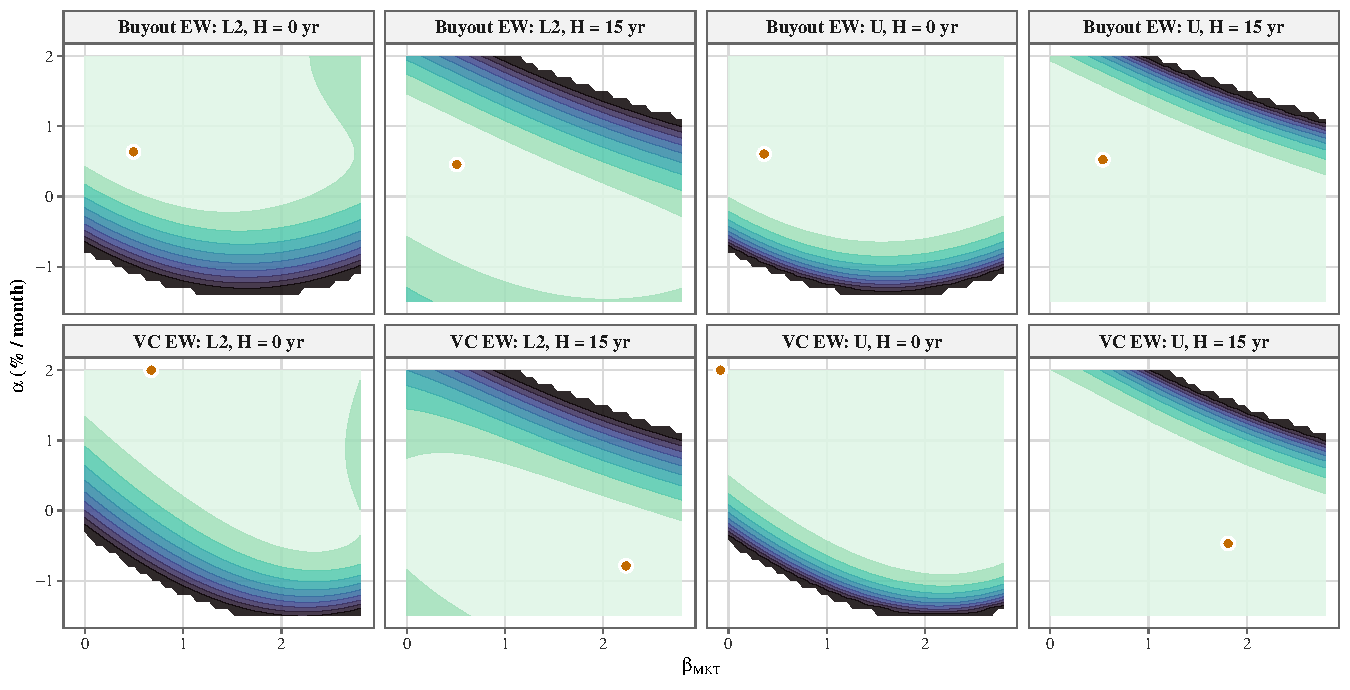
\includegraphics[width=\textwidth]{figure_S5_alpha_beta_contours.pdf}
\caption{Normalized $(\alpha,\beta)$ criterion contours for Buyout and Venture Capital (EW) at $H=0$ and $H=15$ years}
\label{fig:alpha_beta_contours}
\par\vspace{2pt}
{\scriptsize\textit{Notes:} Normalized criterion surfaces $(Q(\alpha,\beta)-Q_{\min})/(Q_{0.90}-Q_{\min})$ over $\beta\in[0,2.8]$ and $\alpha\in[-1.5\%,2\%]$ per month (darker shading = lower criterion; orange circle = constrained optimum on $\Theta$). Top/bottom rows compare Buyout EW (well-defined negatively sloped interior valley reflecting the negative $(\hat\alpha,\hat\beta)$ trade-off) with VC EW (at $H=0$ the surface falls monotonically to the $+2\%$ monthly $\alpha$ upper bound under both L2 and $U_{v,H}$, whereas $H=15$ imposes coercivity without identifying $\alpha$).}
\end{figure}

% Auto-generated by r_project/results/step5_diagnostics.R at commit 731ea2f (uncommitted changes)

\begin{table}[htbp]
\centering
\footnotesize
\caption{Four-year overlapping vintage-block bootstrap versus fixed-$b$ Bartlett confidence intervals (single-factor $\hat\beta_{MKT}$)}
\label{tab:block_bootstrap}
\begin{tabular}{l r rr rr}
\toprule
 & & \multicolumn{2}{c}{Fixed-$b$ Bartlett} & \multicolumn{2}{c}{4-yr block bootstrap ($B=1{,}000$)} \\
\cmidrule(lr){3-4} \cmidrule(lr){5-6}
Estimator, horizon & $\hat\beta$ & SE & 95\% CI & Boot SD & Percentile 95\% CI \\
\midrule
\multicolumn{6}{l}{\textit{Buyout, equally weighted}} \\
\quad $U_{v,H}$ ($q_v=1$), 0 yr & 1.147 & 0.118 & [0.818, 1.476] & 0.149 & [0.929, 1.508] \\
\quad $U_{v,H}$ ($q_v=1$), 15 yr & 1.268 & 0.137 & [0.885, 1.650] & 0.097 & [1.010, 1.401] \\
\quad L2 (VYP), 0 yr & 1.283 & 0.088 & [1.036, 1.530] & 0.134 & [1.075, 1.586] \\
\quad L2 (VYP), 15 yr & 1.108 & 0.060 & [0.942, 1.275] & 0.059 & [0.961, 1.194] \\
\addlinespace
\multicolumn{6}{l}{\textit{Buyout, fund-size weighted}} \\
\quad $U_{v,H}$ ($q_v=1$), 0 yr & 1.197 & 0.143 & [0.799, 1.595] & 0.590 & [1.036, 3.994] \\
\quad $U_{v,H}$ ($q_v=1$), 15 yr & 1.379 & 0.157 & [0.940, 1.818] & 0.119 & [1.117, 1.580] \\
\quad L2 (VYP), 0 yr & 1.224 & 0.126 & [0.874, 1.575] & 0.139 & [1.009, 1.539] \\
\quad L2 (VYP), 15 yr & 0.989 & 0.100 & [0.710, 1.268] & 0.116 & [0.808, 1.244] \\
\addlinespace
\multicolumn{6}{l}{\textit{Venture capital, equally weighted}} \\
\quad $U_{v,H}$ ($q_v=1$), 0 yr & 1.493 & 0.325 & [0.562, 2.425] & 0.329 & [0.745, 1.996] \\
\quad $U_{v,H}$ ($q_v=1$), 15 yr & 1.250 & 0.350 & [0.248, 2.253] & 0.432 & [0.539, 2.030] \\
\quad L2 (VYP), 0 yr & 1.925 & 0.379 & [0.894, 2.956] & 0.415 & [0.958, 2.497] \\
\quad L2 (VYP), 15 yr & 1.270 & 0.410 & [0.155, 2.385] & 0.415 & [0.558, 2.133] \\
\addlinespace
\multicolumn{6}{l}{\textit{Venture capital, fund-size weighted}} \\
\quad $U_{v,H}$ ($q_v=1$), 0 yr & 1.742 & 0.342 & [0.762, 2.722] & 0.429 & [0.707, 2.284] \\
\quad $U_{v,H}$ ($q_v=1$), 15 yr & 1.423 & 0.387 & [0.312, 2.533] & 0.574 & [0.576, 3.010] \\
\quad L2 (VYP), 0 yr & 2.287 & 0.384 & [1.242, 3.333] & 0.563 & [0.898, 2.943] \\
\quad L2 (VYP), 15 yr & 1.595 & 0.485 & [0.273, 2.916] & 0.579 & [0.626, 2.704] \\
\bottomrule
\end{tabular}
\par\vspace{2pt}
{\scriptsize\textit{Notes:} North America complete-history sample ($V\le 2010$). Overlapping 4-year contiguous calendar blocks of vintages are resampled with replacement to match the sample calendar span ($B=1{,}000$ replications), preserving short-range cross-vintage dependence without relying on asymptotic linearization. Fixed-$b$ CIs use Bartlett sandwich SEs ($S=\lceil1.3\sqrt V\rceil$) and Kiefer--Vogelsang critical values. In Buyout FW $U_{v,0}$, 4.6\% of block-bootstrap draws reach the upper bound of $\Theta$ (reflecting the unbounded-below $U_{v,H}$ criterion under small resampled early-vintage weights).}
\end{table}

% Auto-generated by r_project/results/step5_diagnostics.R at commit 731ea2f (uncommitted changes)

\begin{figure}[htbp]
\centering
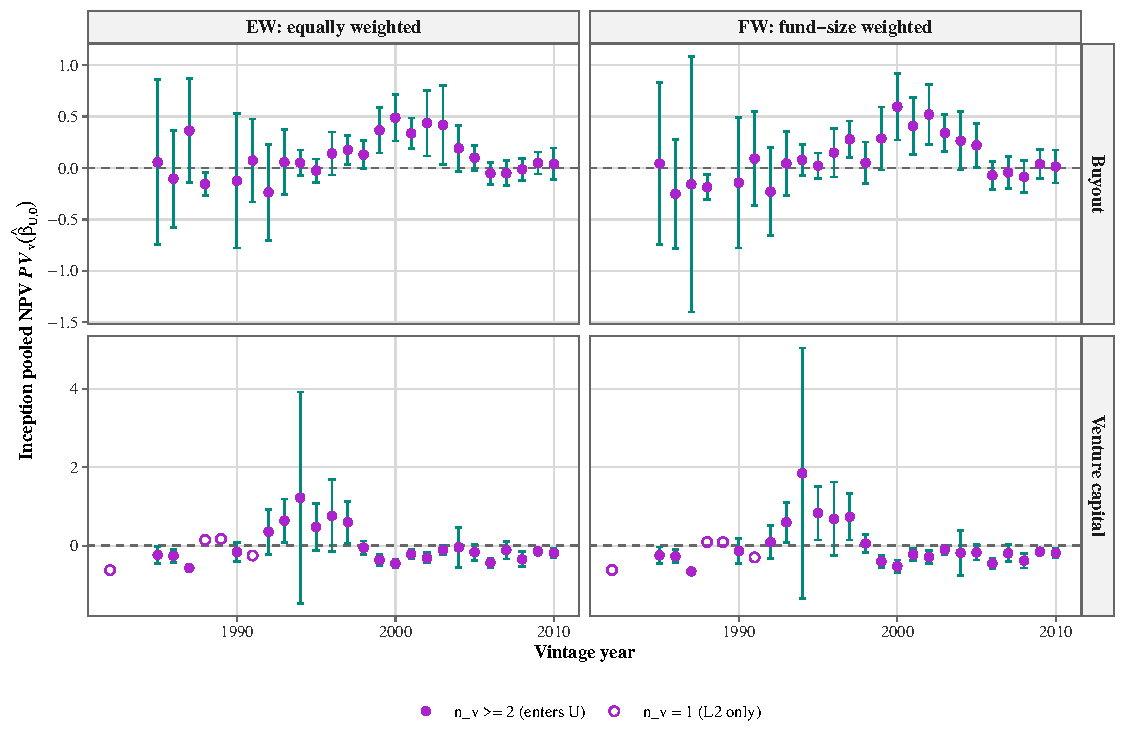
\includegraphics[width=0.92\textwidth]{figure_S5_vintage_residuals.pdf}
\caption{Vintage-level inception pricing errors $PV_v(\hat\beta_{U,0})$ with within-vintage $\pm1.96\,\mathrm{SE}$ bars}
\label{fig:vintage_residuals}
\par\vspace{2pt}
{\scriptsize\textit{Notes:} North America complete-history sample ($V\le 2010$). Each point is the constant-composition vintage portfolio inception NPV evaluated at the headline $U_{v,0}$ ($q_v=1$) single-factor estimate $\hat\beta_{U,0}$. Vertical bars show $\pm 1.96$ within-vintage standard errors of the weighted fund mean for vintages with $n_v\ge 2$ funds; open circles mark singleton vintages ($n_v=1$, entering L2 only). Persistent multi-vintage deviations (notably VC 1993--1997) visually separate vintage-level cohort realizations from within-vintage idiosyncratic dispersion.}
\end{figure}

% Auto-generated by r_project/results/step5_diagnostics.R at commit 4bd0e9c (uncommitted changes)

\begin{table}[htbp]
\centering
\footnotesize
\caption{Vintage-level booked terminal NAV share of total value ($\sum_i \mathrm{NAV}_{i,\mathrm{last}}/\sum_i(\mathrm{DIS}_i + \mathrm{NAV}_{i,\mathrm{last}})$, vintages $\le 2010$)}
\label{tab:terminal_nav_shares}
\begin{tabular}{l r rrrr rr}
\toprule
Series & $V$ & P25 & Median & P75 & Max & Mean $\le 2000$ & Mean 2006--10 \\
\midrule
Buyout, EW & 25 & 3.5\% & 8.1\% & 11.9\% & 18.8\% & 5.6\% & 12.2\% \\
Buyout, FW & 25 & 1.5\% & 5.4\% & 9.2\% & 21.5\% & 4.7\% & 10.7\% \\
Venture capital, EW & 27 & 1.6\% & 10.8\% & 20.6\% & 42.7\% & 5.3\% & 27.1\% \\
Venture capital, FW & 27 & 1.4\% & 8.1\% & 20.0\% & 38.6\% & 5.3\% & 24.2\% \\
\bottomrule
\end{tabular}
\par\vspace{2pt}
{\scriptsize\textit{Notes:} North America complete-history sample ($V\le 2010$). For each vintage, booked terminal NAV share sums every fund's own final reported NAV (booked as a liquidating distribution in the cash-flow panel) divided by total distributions plus booked terminal NAV (equal-weighted in EW, fund-size-weighted in FW). Per-vintage values are stored in \texttt{vintage\_terminal\_nav\_shares.csv}.}
\end{table}

\begin{figure}[htbp]
\centering
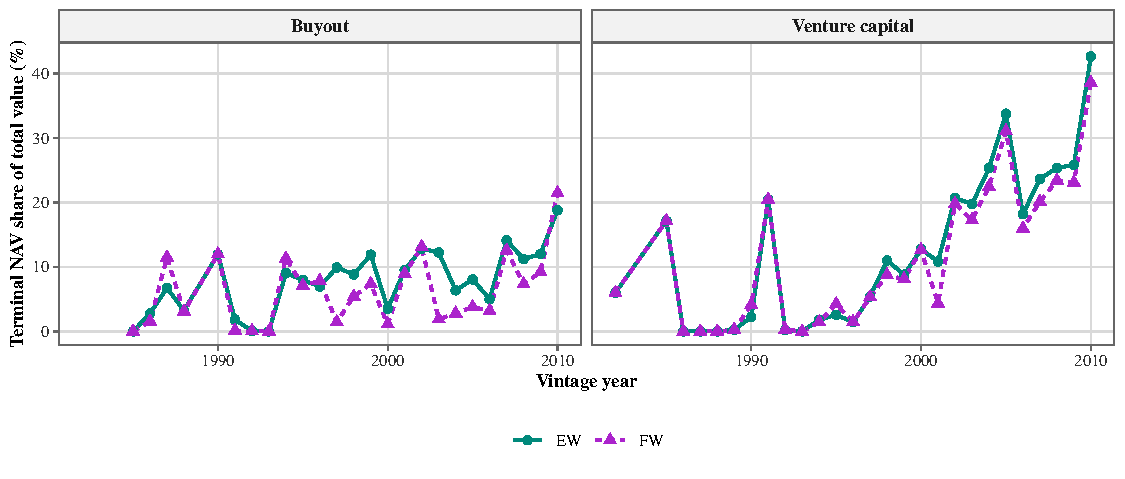
\includegraphics[width=0.88\textwidth]{figure_S5_terminal_nav_shares.pdf}
\caption{Vintage-level booked terminal NAV shares of total value ($V \le 2010$).}
\label{fig:terminal_nav_shares}
\end{figure}
% Auto-generated by r_project/results/appendix_e_cv_folds.R at commit 8585b0d (uncommitted changes)

\begin{table}[htbp]
\centering
\footnotesize
\caption{Cross-validation fold diagnostics ($hv$-block CV): fold stability and common $H=0$ held-out loss (B7/B8)}
\label{tab:appendix_e_cv_folds}
\begin{tabular}{l rrrr r rr}
\toprule
Horizon & Full $\hat\beta$ & Fold mean & $\mathrm{SD}_{CV}$ & $\mathrm{SR}_{CV}$ & Bound folds & Val.\ loss ($H$) & Val.\ loss ($H=0$) \\
\midrule
\multicolumn{8}{l}{\textit{Buyout, equally weighted (single-factor MKT, 8 folds)}} \\
\quad 0 yr & 1.283 & 1.294 & 0.061 & 20.90 & 0 & 0.109 & 0.109 \\
\quad 5 yr & 1.259 & 1.275 & 0.075 & 16.73 & 0 & 0.139 & 0.108 \\
\quad 10 yr & 1.157 & 1.186 & 0.094 & 12.31 & 0 & 0.188 & 0.108 \\
\quad 15 yr & 1.108 & 1.131 & 0.063 & 17.58 & 0 & 0.234 & 0.107 \\
\quad 20 yr & 1.018 & 1.034 & 0.063 & 16.20 & 0 & 0.270 & 0.106 \\
\quad 30 yr & 0.933 & 0.954 & 0.078 & 12.02 & 0 & 0.334 & 0.113 \\
\addlinespace
\multicolumn{8}{l}{\textit{Buyout, fund-size weighted (single-factor MKT, 8 folds)}} \\
\quad 0 yr & 1.224 & 1.201 & 0.096 & 12.77 & 0 & 0.117 & 0.117 \\
\quad 5 yr & 1.218 & 1.206 & 0.110 & 11.03 & 0 & 0.152 & 0.118 \\
\quad 10 yr & 1.108 & 1.111 & 0.112 & 9.91 & 0 & 0.208 & 0.121 \\
\quad 15 yr & 0.989 & 0.990 & 0.102 & 9.71 & 0 & 0.275 & 0.131 \\
\quad 20 yr & 0.880 & 0.874 & 0.052 & 16.77 & 0 & 0.321 & 0.138 \\
\quad 30 yr & 0.798 & 0.791 & 0.038 & 21.27 & 0 & 0.384 & 0.148 \\
\addlinespace
\multicolumn{8}{l}{\textit{Venture capital, equally weighted (single-factor MKT, 8 folds)}} \\
\quad 0 yr & 1.925 & 1.743 & 0.575 & 3.35 & 0 & 0.303 & 0.303 \\
\quad 5 yr & 2.145 & 1.795 & 0.678 & 3.16 & 0 & 0.479 & 0.327 \\
\quad 10 yr & 1.710 & 1.483 & 0.540 & 3.17 & 0 & 0.651 & 0.327 \\
\quad 15 yr & 1.270 & 1.075 & 0.391 & 3.24 & 0 & 0.716 & 0.347 \\
\quad 20 yr & 0.943 & 0.744 & 0.293 & 3.22 & 0 & 0.772 & 0.391 \\
\quad 30 yr & -0.373 & -0.332 & 0.338 & -1.10 & 0 & 1.195 & 1.106 \\
\addlinespace
\multicolumn{8}{l}{\textit{Venture capital, fund-size weighted (single-factor MKT, 8 folds)}} \\
\quad 0 yr & 2.287 & 1.989 & 0.708 & 3.23 & 0 & 0.375 & 0.375 \\
\quad 5 yr & 2.472 & 1.994 & 0.790 & 3.13 & 0 & 0.615 & 0.400 \\
\quad 10 yr & 2.066 & 1.740 & 0.697 & 2.96 & 0 & 0.869 & 0.407 \\
\quad 15 yr & 1.595 & 1.326 & 0.565 & 2.82 & 0 & 0.979 & 0.444 \\
\quad 20 yr & 1.239 & 0.962 & 0.449 & 2.76 & 0 & 1.034 & 0.501 \\
\quad 30 yr & -0.573 & -0.437 & 0.416 & -1.38 & 0 & 1.563 & 1.580 \\
\bottomrule
\end{tabular}
\par\vspace{2pt}
{\scriptsize\textit{Notes:} North America complete-history sample ($V\le 2010$), L2 on constant-composition vintage portfolios. Eight 3-year $hv$-block folds (validation windows 1988--1990 through 2009--2010, buffered by 3-year blocks on each side). $\mathrm{SD}_{CV}$ is the cross-fold standard deviation (descriptive stability diagnostic, not a sampling SE); $\mathrm{SR}_{CV}=\hat\beta_{\mathrm{full}}/\mathrm{SD}_{CV}$ (B7). Val.\ loss ($H$) averages held-out horizon-$H$ loss; Val.\ loss ($H=0$) evaluates every horizon's fold estimates on the common $H=0$ held-out loss so horizons are directly comparable (B8). Joint $(\alpha,\beta)$ fold diagnostics are stored in \texttt{appendix\_e\_cv\_folds.csv}.}
\end{table}

\begin{figure}[htbp]
\centering
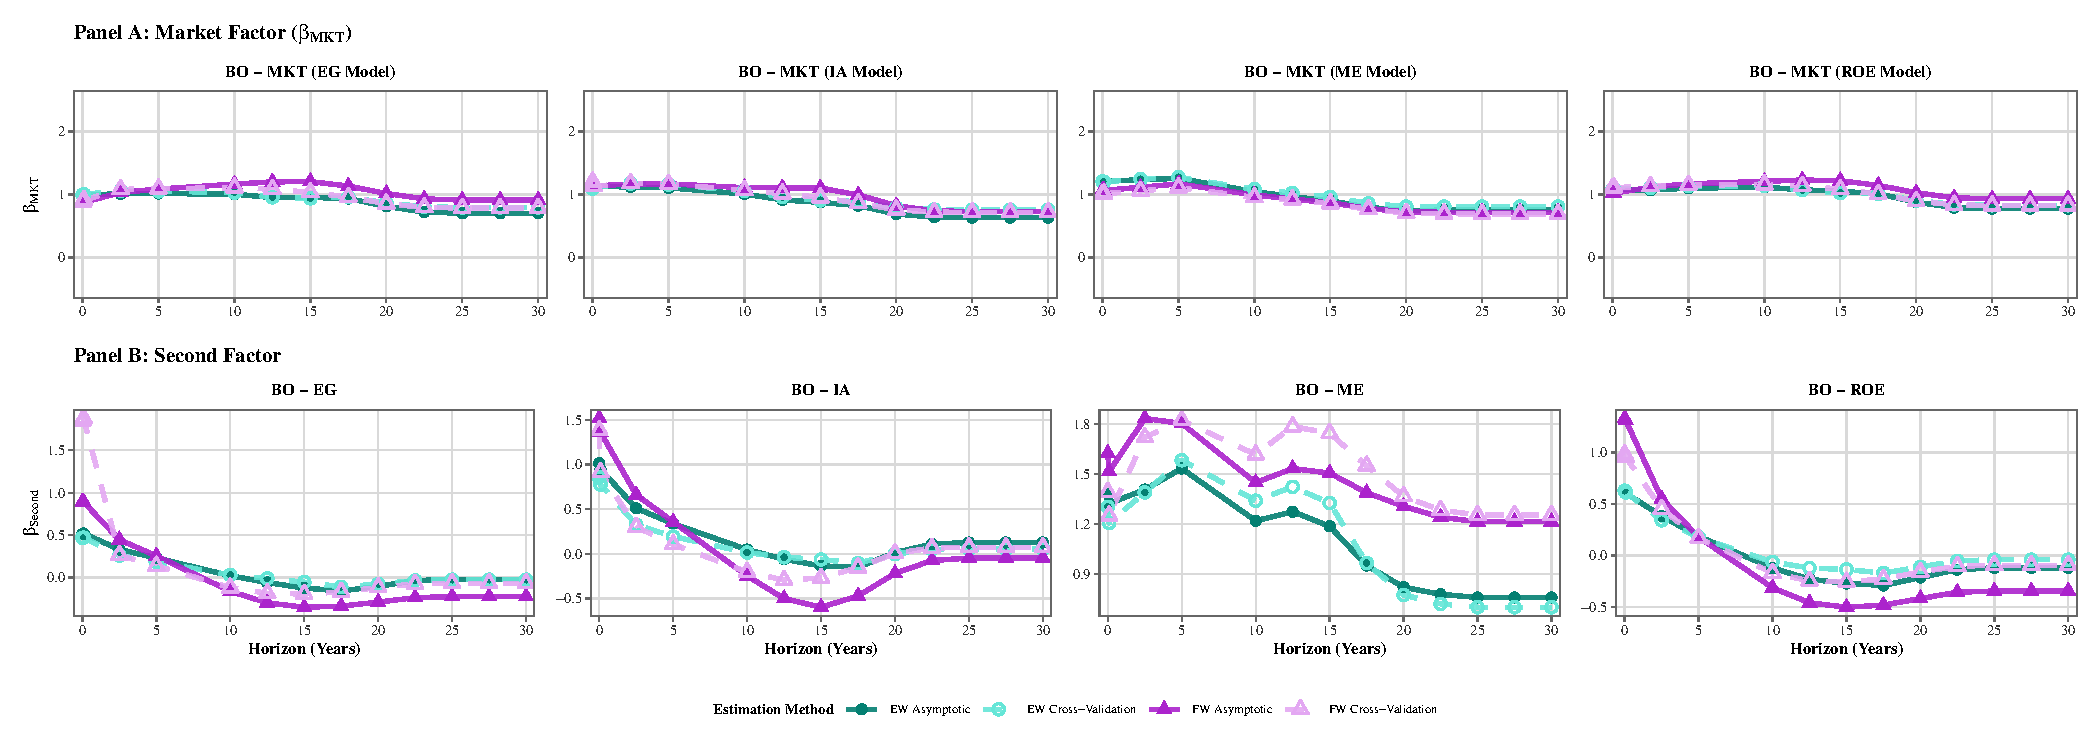
\includegraphics[width=0.99\textwidth]{empirical_BO_US_Multi.pdf}
\caption{\textbf{Two-factor $q^5$ L2 estimates for Buyout ($V \le 2010$).} Market loading (top row) and second-factor loading (bottom row) across horizons for MKT paired with EG, IA, ME, and ROE under EW and FW.}
\label{fig:empirical_BO_q_factors}
\end{figure}
\begin{figure}[htbp]
\centering
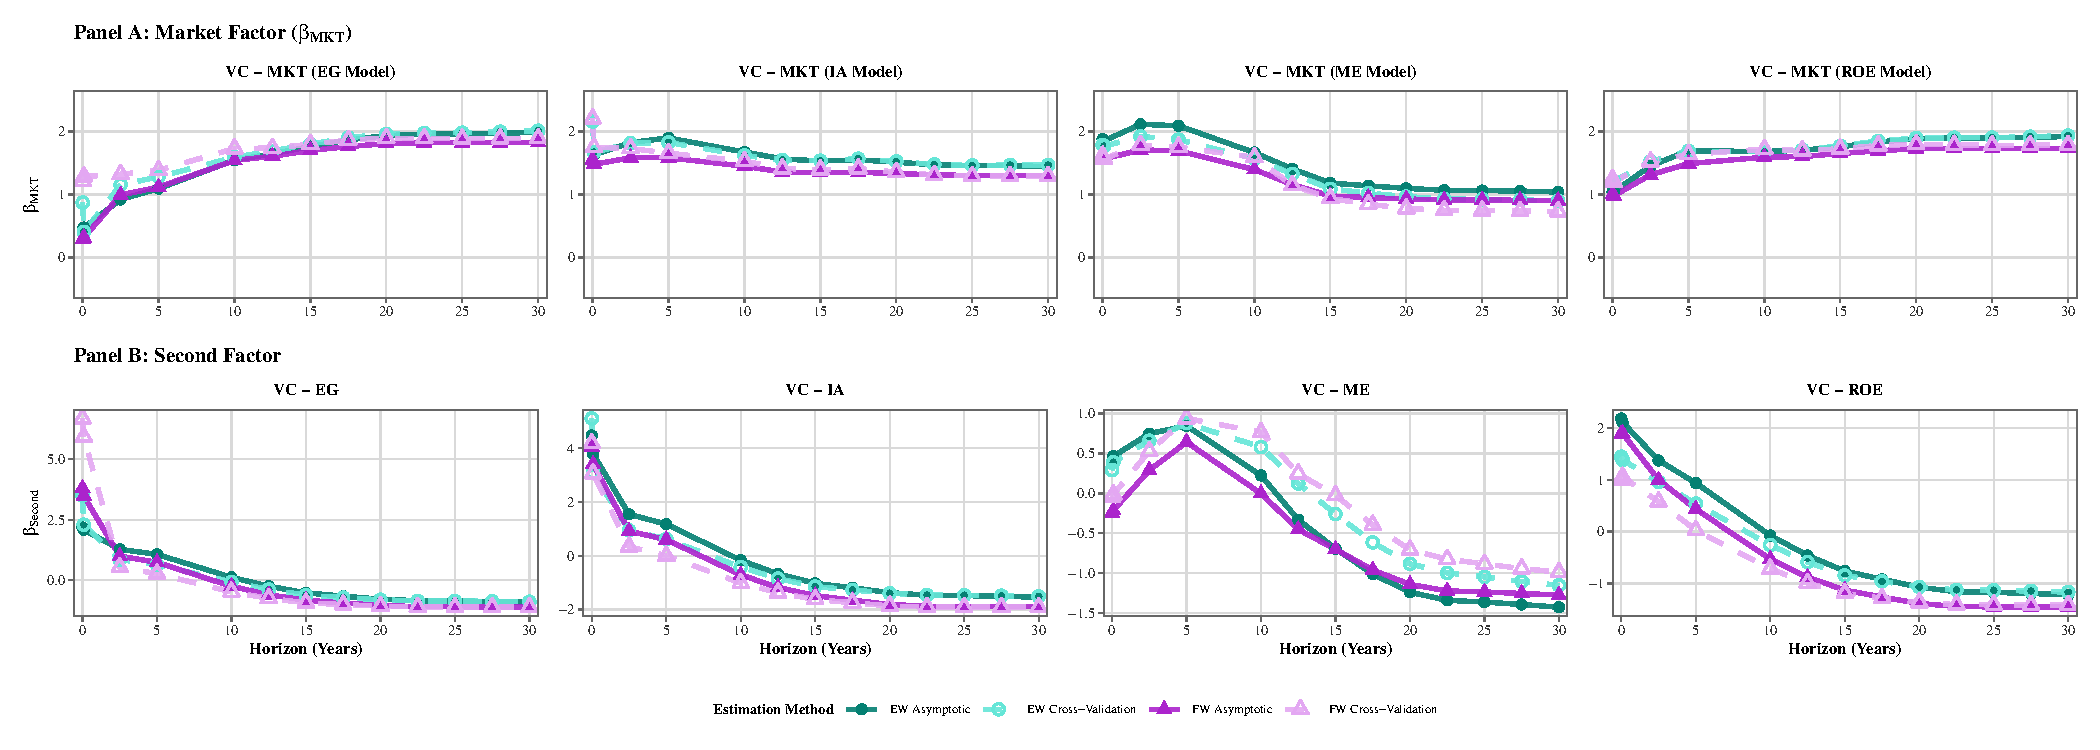
\includegraphics[width=0.99\textwidth]{empirical_VC_US_Multi.pdf}
\caption{\textbf{Two-factor $q^5$ L2 estimates for Venture Capital ($V \le 2010$).} Market loading (top row) and second-factor loading (bottom row) across horizons for MKT paired with EG, IA, ME, and ROE under EW and FW.}
\label{fig:empirical_VC_q_factors}
\end{figure}
% Auto-generated by r_project/results/table_published_estimates.R at commit 731ea2f (uncommitted changes)

\begin{table}[htbp]
\centering
\footnotesize
\caption{Comparison of Buyout and Venture Capital systematic risk ($\beta$) and abnormal performance estimates across the literature}
\label{tab:published_estimates}
\resizebox{\linewidth}{!}{%
\begin{tabular}{l l l l l l}
\toprule
Study & Data (vintages) & Method & Buyout $\beta_{MKT}$ & VC $\beta_{MKT}$ & Abnormal performance ($\alpha$ / PME) \\
\midrule
\multicolumn{6}{l}{\textit{Panel A: This paper (North America USD, Preqin complete histories, $V\le 2010$, $H=0$)}} \\
This paper, $U_{v,0}$ (EW, main) & Preqin (1982--2010) & Pair-product $U_{v,0}$ ($q_v=1$) & 1.147 (0.118) & 1.493 (0.325) & BO $\hat\beta$=0.362, $\hat\alpha$=0.605\%/mo; VC bound \\
This paper, $U_{v,0}$ (FW, main) & Preqin (1982--2010) & Pair-product $U_{v,0}$ ($q_v=1$) & 1.197 (0.143) & 1.742 (0.342) & BO $\hat\beta$=0.439, $\hat\alpha$=0.568\%/mo; VC bound \\
This paper, L2 (EW, benchmark) & Preqin (1982--2010) & Pooled squared NPV ($H=0$) & 1.283 (0.088) & 1.925 (0.379) & Noise-tilted upward (T3/T4) \\
This paper, L2 (FW, benchmark) & Preqin (1982--2010) & Pooled squared NPV ($H=0$) & 1.224 (0.126) & 2.287 (0.384) & Noise-tilted upward (T3/T4) \\
\midrule
\multicolumn{6}{l}{\textit{Panel B: Selected published cash-flow and secondary-market studies}} \\
\cite{DLP12} & TVE (1980--1993) & Pooled NPV GMM ($H=0$) & 1.31 (1-f); 0.72 (4-f) & 2.73 (1-f); 2.20 (4-f) & BO $-4.8\%$/yr (insig.); VC $-12.3\%$/yr \\
\cite{FNP12} & CEPRES deals (1975--2006) & Deal-level IRR / SDF & 1.30--1.40 & -- & Zero / modest after liquidity risk \\
\cite{HJK14} & Burgiss (1984--2008) & KS-PME ($\beta\equiv 1$) & 1.00 (imposed) & 1.00 (imposed) & BO PME $\approx 1.20$; VC PME $\approx 1.36$ (90s) / $<1$ (00s) \\
\cite{KN16} & Preqin (1982--2008) & Public-SDF GPME & -- & $\approx 1.0$--$2.0$ (state-dep.) & VC GPME $\approx 0$ (insig. post-1999) \\
\cite{RS16} & LP cash flows (1984--2010) & Tailored PME / IRR & $\approx 1.0$--$1.3$ & $\approx 1.0$--$1.5$ & BO PME $\approx 1.18$; VC PME $\approx 1.03$ \\
\cite{ACGP18} & Preqin (1994--2015) & Bayesian LP cash-flow panel & $\approx 1.3$ & $\approx 1.6$--$1.8$ & Cyclical; modest net average $\alpha$ \\
\cite{GN18} & Preqin (1981--2016) & Cash-flow strip replication & Small-value strip & Growth strip & Negative average risk-adjusted profit \\
\cite{boyer2023discount} & Secondary txns (2006--2018) & Transaction-based index & 1.75--1.79 & High (levered growth) & Near-zero CAPM $\alpha$ (discount-rate risk) \\
\cite{KN24} & Preqin / Burgiss (1984--2016) & Public-SDF direct $\alpha$ & $\approx 0.9$--$1.1$ & $>1$ (high dispersion) & BO positive; VC near zero / negative post-1999 \\
\bottomrule
\end{tabular}%
}
\par\vspace{2pt}
{\scriptsize\textit{Notes:} Panel~A reports single-factor $\hat\beta_{MKT}$ (Bartlett sandwich SE in parentheses) from Table~\ref{tab:u_l2_beta} and joint $(\alpha,\beta)$ estimates from Table~\ref{tab:u_l2_alpha_beta}; VC $(\alpha,\beta)$ at $H=0$ sits on the $+2\%$ monthly $\alpha$ bound due to the 1993--1997 cohort (Table~\ref{tab:vc_without_1993_1997}). Panel~B summarizes representative findings from the private-equity cash-flow and secondary-market pricing literature; methodologies differ in whether $\beta$ is estimated jointly with $\alpha$, whether a public-calibrated SDF or PE-specific benchmark deflator is used (Appendix~\ref{sec:appendix_sdf}), and in underlying data vendor and sample window.}
\end{table}



\newpage
\singlespacing
\bibliographystyle{apalike}
\bibliography{sdf_paper_refs}

\end{document}
